\documentclass[table]{elegantpaper}
\usepackage{datetime2}
\usepackage[T1]{fontenc}
\usepackage{graphicx}
\usepackage{svg}
\usepackage{listings}
\usepackage{listings-rust}
\usepackage{pgf-pie}
\usepackage{rotating}
\usepackage{tabularray}
\usepackage{tabularx}
\usepackage{makecell}
\usepackage{color}
\usepackage{changepage}
\usepackage{xcolor}
\usepackage{titlesec}

\titleclass{\subsubsubsection}{straight}[\subsection]

\newcounter{subsubsubsection}[subsubsection]
\renewcommand\thesubsubsubsection{\thesubsubsection.\arabic{subsubsubsection}}
\renewcommand\theparagraph{\thesubsubsubsection.\arabic{subsubsubsection}} % optional; useful if paragraphs are to be numbered

\titleformat{\subsubsubsection}
  {\normalfont\normalsize\bfseries}{\thesubsubsubsection}{1em}{}
\titlespacing*{\subsubsubsection}
{0pt}{3.25ex plus 1ex minus .2ex}{1.5ex plus .2ex}

\makeatletter
\renewcommand\subsubsubsection{\@startsection{subsubsubsection}{5}{\z@}%
  {3.25ex \@plus1ex \@minus.2ex}%
  {-1em}%
  {\normalfont\normalsize\bfseries}}
\renewcommand\subparagraph{\@startsection{subparagraph}{6}{\parindent}%
  {3.25ex \@plus1ex \@minus .2ex}%
  {-1em}%
  {\normalfont\normalsize\bfseries}}
\def\toclevel@subsubsubsection{4}
\def\toclevel@subsubsubsection{5}
\def\toclevel@subsubsubsection{6}
\def\l@subsubsubsection{\@dottedtocline{4}{7em}{4em}}
\def\l@subsubsubsection{\@dottedtocline{5}{10em}{5em}}
\def\l@subparagraph{\@dottedtocline{6}{14em}{6em}}
\makeatother

\setcounter{secnumdepth}{5}
\setcounter{tocdepth}{5}

\DTMusemodule{english}{en-GB}
\DTMnewdatestyle{short}{
  \renewcommand{\DTMdisplaydate}[4]{
    \DTMenglishmonthname{##2} \number##1\relax
  }
  \renewcommand{\DTMDisplaydate}{\DTMdisplaydate}
}
\newcommand{\shorttoday}{{\DTMsetdatestyle{short}\today}}
\renewcommand{\updatetext}{}

\graphicspath{{./images/}}
\DeclareEmphSequence{\bfseries,\itshape,\upshape}
\lstset{xleftmargin=\parindent,xrightmargin=\parindent}

\title{Ola: A Privacy First ZKVM}
\author{Sin7Y, Applied R\&D Team\thanks{\url{https://twitter.com/Sin7Y_Labs}}}
\date{\shorttoday}

\addbibresource[location=local]{reference.bib}

\begin{document}
    \maketitle
    \begin{abstract} 

    \noindent We are developing a ZK-ZKVM platform for Ethereum\cite{website:Ethereum} that will offer the following features: 
    (1) Programmable Privacy: unlike specific privacy, Ola could private for everything which supports user-defined functions; 
    (2) Optional Privacy: both the project side and user side could optionally choose to deploy/send public/private type; 
    (3) Compliance-friendly Privacy: Through the means of viewing keys that can be shared with third parties, we create a compliance-friendly landscape, providing the possibility for 
    regulators to track the private assets, avoiding the disadvantages of untraceable assets, such as Tornado Cash\cite{website:Tornado-cash}; 
    (4) High Programmability: a customize GPL language which has more advanced features and is more programmable than DSL\cite{website:DSL}; 
    (5) High Performance: customize full-featured zk-friendly ZKVM, OlaVM\cite{website:OlaVM}, can quickly execute transactions and generate proofs; 
    (6) Developer-friendly language: Ola-lang\cite{website:Ola-lang}  is customized for smart contract development with syntax similar to Rust, making it convenient for developers quickly adopt it; 
    (7) Developer-friendly IDE: Ola-lang language is integrated into the Visual Studio Code, making it convenient for traditional developers to start building;
    (8) Better Scalability: based on the LLVM compilation framework, it is easier to achieve compatibility with other advanced programming languages; 
    (9) Uptable view key: avoiding third-party continuous monitoring and tracking of an account's status; 
    (10) Data ownership: taking the control of their asset information and on-chain data.
    \\ \hspace*{\fill} \\
    \noindent Ola is a rapidly developing project and this is the second whitepaper that will describe the design philosophy and specifications of our full-featured zk-friendly ZKVM,  
    OlaVM\cite{website:OlaVM} and developer-friendly general purpose smart contract language, Ola-lang\cite{website:Ola-lang} detailedly. Implementation details related to privacy will be released in the upcoming third whitepaper upon releasing the test net.
    \\ \hspace*{\fill} \\
    \noindent \textbf{Key words: Privacy, Programmability, ZKVM, Smart Contract, Data Ownership.}    
\end{abstract}
    \tableofcontents
    \section{Introduction}\label{sec:introduction}

In the past few years, we have witnessed a rapid development of the blockchain industry, influx of capital, users, and builders has enabled unprecedented growth and potential of the entire industry. However, blockchain is still somewhat in its infancy, infrastructure is still maturing. One of the largest challenges is the low transactional throughput of public blockchain systems, especially the largest public programmable blockchain Ethereum \cite{website:Ethereum}, which in the best case scenario \cite{website:Etherscan-chart}, processes up to 23 transactions per second, far less than traditional centralized systems. 

There are many reasons for the congestion of the Ethereum network, such as the POW \cite{website:POW} consensus algorithm (The Merge upgrade \cite{website:The-Merge} to POS \cite{website:POS} consensus now), the repeated execution of verification process of all transactions by nodes, and the serial execution of transactions; for the above reasons, many projects are trying to scale Ethereum through different means. Approach 1: Launching new public blockchains, independent of Ethereum, using faster consensus algorithms or faster transaction execution to achieve higher TPS, such as BSC \cite{website:BSC}, Solana \cite{website:Solana}, Aptos \cite{website:Aptos}, etc; Approach 2: Ethereum Sidechain, using faster consensus algorithms and then regularly synchronizing to Ethereum, such as Polygon \cite{website:Polygon}, Optimism \cite{website:Optimism}, Arbitrum \cite{website:Arbitrum}, etc; Approach 3: ZK(E)VM, a Layer2 network of Ethereum, using ZK technology to solve the problem of repeated execution of transactions, such as Polygon Hermez \cite{website:Polygon-Hermez}, Zksync \cite{website:Zksync} etc.

Scaling is not the only problem that has to be solved in the long term for Ethereum and the wider blockchain space. There are many excellent teams working rigorously on scaling solutions, the ola team believe that the next crucial feature to be implemented is privacy. Blockchains being a public ledger, all transactions taking place on-chain, meaning state changes containing the asset information related to an address or account is open and transparent. 

Excessive information transparency leads to: 

\begin{enumerate}
    \item MEV (Maximal Extractable Value) issues. Miners can selectively package transactions based on its fee, resulting in transactions with lower fees having a lower likelihood of being processed, if ever, forcing users to increase their fees. More concerning:
    \item Front running and censorship attacks, through the means of MEV. Block producers in programmable blockchains can use MEV to exploit certain smart contracts deployed on the blockchain (Such as DEXes and other DeFi products). They may also censor certain addresses. Such an attack could be that the miner or block producer sees a buy order in the memory pool (where transactions that are not yet appended to the blockchain are stored) and adds their own buy order on that particular DEX, thus increasing the price of the given token. The other transaction that is added is a sell order of given token and the third order is the buy order of the third party for the new increased price. Resulting in huge security issues and in the past year hackers have managed to steal assets roughly amounting to 2 billion dollars.
    \item User data ownership problems, both the assets information and transaction information of addresses are open to being monitored and used, which is contrary to the vision of Web3 \cite{website:Web3}. Therefore, when the scaling problem is solved, privacy will become the next urgent feature to achieve. In the world of blockchain, privacy is not a new topic, it has long been studied and supported by the Zcash team \cite{website:Zcash}.
\end{enumerate}

\subsection{Non Programmable Privacy}

In addition to the Zcash team, other public blockchains that implement private transactions include Monero \cite{website:Monero}, Dash \cite{website:Dash}, Grin \cite{website:Grin}, and others. However, these public chains lack programmability and can only be used for simple private transfer of assets. Consequently, their ecosystem development lags far behind Ethereum, which has become the largest public chain in the ecosystem due to its programmability, but Ethereum lacks privacy features.

Therefore, some projects have begun to explore ways to introduce privacy to Ethereum, such as the ZK-ZKRollup application zk.money \cite{website:zk.money} developed by the Aztec \cite{website:Aztec} team. However, the current zk.money product has been discontinued, mainly because it's privacy features only apply to simple single transfer scenarios. Given the current explosion of Defi applications, asset transfer is only one of the simplest financial scenarios, and therefore the user base is limited, while the maintenance costs continue to accrue.
\begin{figure}[!ht]
    \centering
    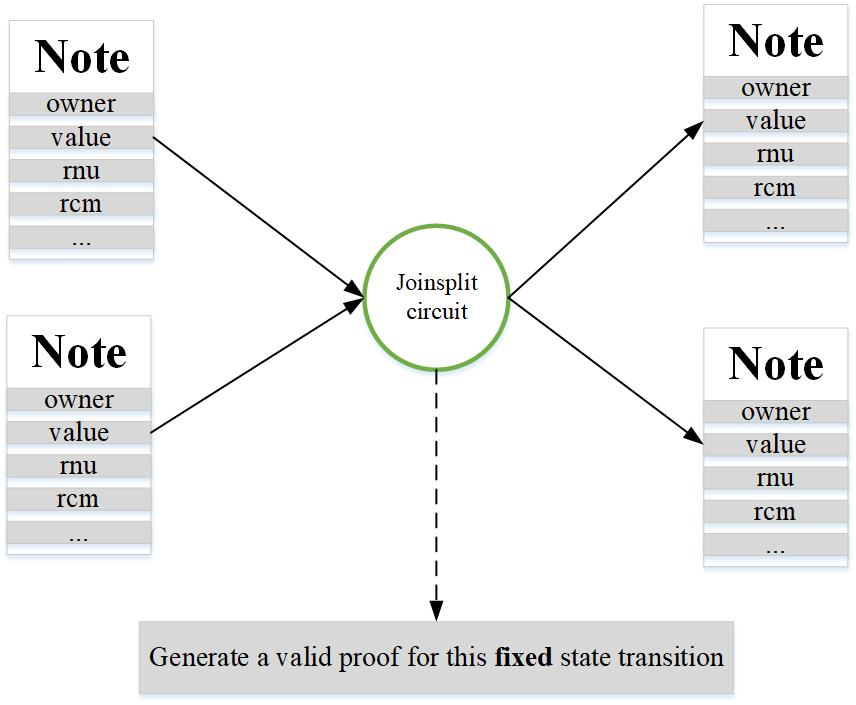
\includegraphics[width=0.4\textwidth]{Example of Non Programmable privacy.jpg}
    \caption{Example of Non Programmable Privacy}
    \label{fig:Example of Non Programmable Privacy}
\end{figure}

\figref{fig:Example of Non Programmable privacy} shows the simple logic of non programmable privacy. The value change logic corresponding to the input and output notes in Section \ref{section: sending-notes} are also fixed, generally in the form of ``A + B = C + D''. Manta Network \cite{website:Manta-network} is a public blockchain that supports user-defined token privacy transfers, and the privacy transaction 
constraint circuits of all fungible tokens can be used to reuse the above logic.

A ZK-ZKRollup application of a single scenario use case, is similar to a ZKRollup application of a single scenario use case. If you want to use the asset in other applications or for other use cases, you must cross the asset to another application through a bridge, which brings with it very poor user experience. Therefore, just as ZKRollups need to 
transition to ZK(E)VMs, ZK-ZKRollup also need to transition to ZK-ZKVMs (Appendix \ref{section: solidity-compatibility} explains how to get solidity compatibility).

\subsection{Programmable Privacy}

ZK-ZKVM has two main features (1) It's a privacy-first platform, not privacy-only. This means that users can choose the transaction type, public or private, depending on their need. Just similar to the Zcash;
(2) Programmability, you can deploy any smart contract, public or private, depending on the needs of the project side. Compared with non programmable privacy, the main difference is the logic of state transition in a note \ref{section: sending-notes}, \figref{fig:Difference between Non Programmable Privacy and Programmable Privacy} simply shows the difference 

\begin{figure}[!ht]
    \centering
    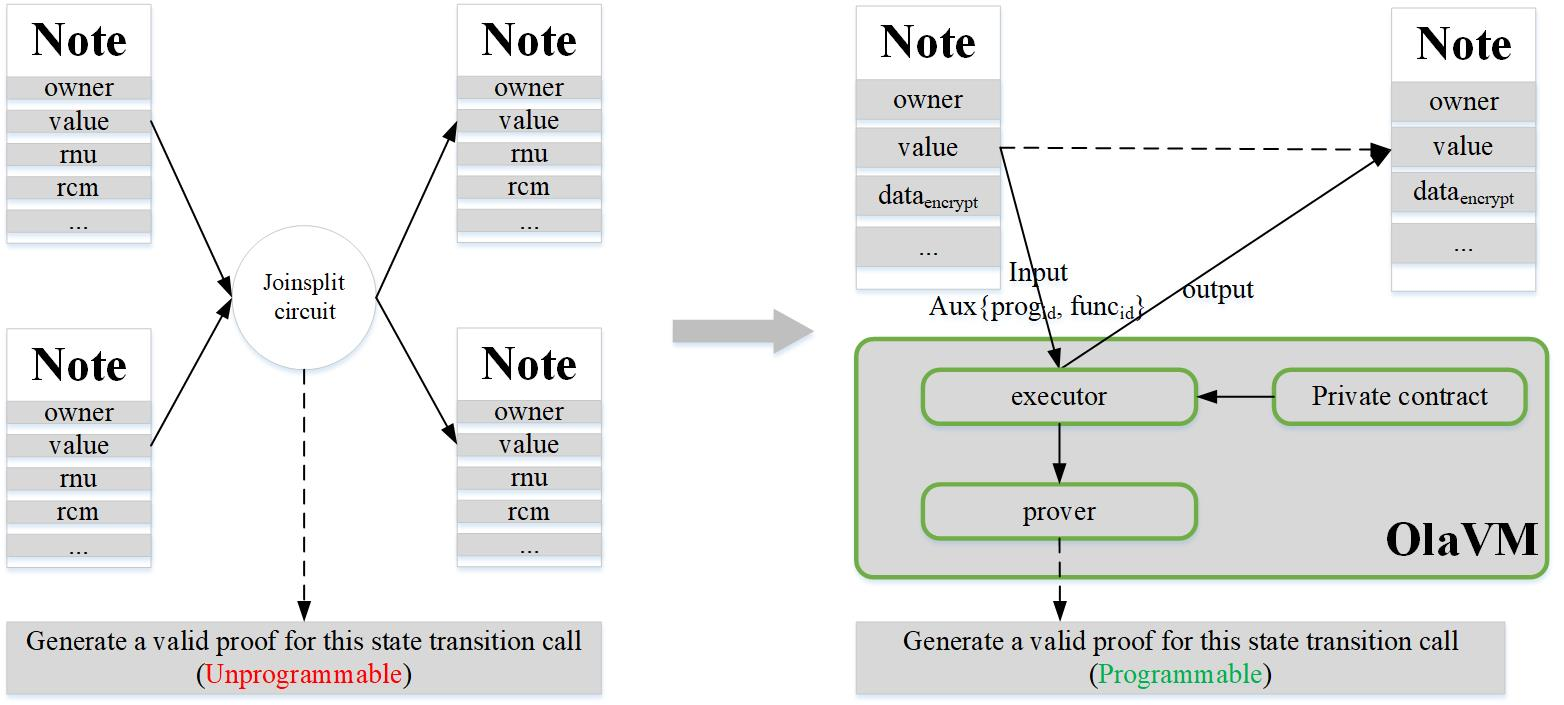
\includegraphics[width=0.6\textwidth]{Difference between Non Programmable Privacy and Programmable Privacy.jpg}
    \caption{Difference between Non Programmable Privacy and Programmable Privacy}
    \label{fig:Difference between Non Programmable Privacy and Programmable Privacy}
\end{figure}

The current projects focusing on programmable privacy are Aleo \cite{website:Aleo} and Aztec. Aleo is a 
privacy-first public blockchain, from Bitcoin \cite{website:BTC} to Ethereum to Zcash \cite{website:Zcash} to Aleo. It brings the public blockchain into a new era,
supporting programmable privacy. 
It has reached the testnet stage and supports developers to deploy privacy contracts on it; 
Aztec focuses on doing Layer2 programmable privacy for Ethereum, a project 
called Aztec3 \cite{website:Aztec3}, is still in development.

Before we clarify the different approaches to get programmability, we should give some explanations on Domain Specific Language (DSL) and General Purpose Language (GPL) \cite{website:DSL}.
DSL is defined as a computer programming language of limited expressiveness focused on a particular domain, limited expressiveness means it just supports a bare minimum of features 
needed to support its domain. You can't build an entire software system in a DSL; rather, you use a DSL for one particular aspect of a system. While GPL is defined as a general-purpose programming language

So there are often two ways to achieve programmability, one is to design a DSL, such as Circom \cite{website:Circom}, Pil \cite{website:Pil}, Noir \cite{website:Noir}, etc; the other is SCL, 
such as Cairo1.0 \cite{website:Cairo1.0}, Solidity \cite{website:Solidity}, Ola lang \cite{website:Ola-lang} and so on. As we have mentioned before, the main difference is that SCL supports more complex structures and has 
higher abstraction, it's more suitable for writing complex business logic and meanwhile, and DSL is more suitable for some simple computational expressions. 
Take Pil \cite{website:Pil} language as an example, you can directly use it to define a simple micro-op, such as ``A * B + C'', or ``A * B * C + D'' and other simple combinations. 
\tabref{table:Difference between DSL and SCL} briefly shows some of the differences between DSL and SCL.

\begin{table}[!ht]
    \centering
    \begin{tabular}{|c|c|c|c|c|c|}
        \hline
        \emph{Type} & \emph{Abstraction} & \emph{Process} & \emph{Difficulty} & \emph{Examples} & \emph{Notes} \\ 
        \hline
        DSL & low & program -> arith-ops -> ops gadgets & normal & \makecell{circom \\ noir \\ cairo} & \makecell{1. semantic analysis \\ 2. codeGen optimization} \\
        \hline
        \makecell{SCL \\ (ISA/VM)} & high & program -> bytecodes -> cpu circuit & hard & \makecell{solidity \\ cairo1.0 \\ ola lang} & \makecell{1. need a compiler \\2. re-use LLVM framework} \\
        \hline
    \end{tabular}
    \caption{Difference between DSL and SCL}
    \label{table:Difference between DSL and SCL}
\end{table}

If you want to prove a program written by DSL is executed correctly (this is what ZKDSL means), you may need to predefine some common operators, each of them corresponding to a circuit, called a gadget \cite{website:Gadget}. 
Developers can use these operators to implement desired functions, but it's difficult to handle the call and return logic between functions. Meanwhile, If you want to prove a program written by SCL is executed correctly (this is what ZKVM means), 
 you need to design corresponding constraints for each instruction, collectively referred to as CPU circuit; therefore, Any program will be compiled into 
 bytecodes composed of these instructions, and then constrained by the CPU circuit.

Ola achieved a customized SCL to get programmability even though it's harder to implement than DSL, because we could get benefits from it as follows:
 \begin{itemize}
 \item A higher abstraction and programmable language, allowing developers to write smart contracts with arbitrary logic;
 \item A full-featured zk-friendly VM can be designed to achieve higher system performance;
 \item LLVM-based compiler can be more easily compatible with other advanced programming languages.
\end{itemize}

\subsection{Full-featured ZK-friendly ZKVM}

As mentioned earlier, the best way to achieve programmability is to design a ZKVM with a custom Instruction Set Architecture, a custom smart contract language, and a custom compilation, etc. 
ZKVM is a virtual machine that can execute any program and at the same time generate a zero-knowledge proof of the correctness of the execution process. Therefore, the speed of proof generation 
is very critical, and it will directly affect the performance of the entire system.

The key to obtaining a full-featured zk-friendly ZKVM is how to obtain(1)the smallest execution trajectory; (2)the most concise state transition constraint logic; (3)the fastest 
zero-knowledge proof algorithm. The smallest execution trajectory means: for the same computational logic, OlaVM \cite{website:OlaVM} can be expressed with the least instructions, the main technical means are the 
support for non-deterministic computation at the computational level, and the register-based design is used at the memory access level; The most concise state transition constraint logic means: 
for the same computational logic, OlaVM \cite{website:OlaVM} can constrain the entire execution trajectory with the least polynomials and the smallest order. The main means is to obtain the instruction with the least 
number of instructions through the Algebraic RISC architecture. The number of Instruction Set Architecture determines the complexity of Cpu constraints; faster zero-knowledge proof algorithm 
Meaning: For the same calculation, OlaVM \cite{website:OlaVM} can complete the proof generation process in less time, which mainly depends on the Godilocks \cite{website:Goldilocks} field, a finite field less than 64bit, compared to the 
SNARK system based on large bit width elements of elliptic curves, based on The STARK algorithm of the Goldilocks \cite{website:Goldilocks} field can be executed faster.

Subsequent chapters will explain in detail Ola's design philosophy and design specifications for obtaining a Full-featured ZK-friendly ZKVM. As the first programmable privacy layer network 
based on ZKVM, Ola will support the following scenarios for different subjects:

\begin{itemize}
\item For Developers
    \begin{itemize}
    \item Developers can freely choose to deploy public contracts(Account-based), privacy contracts(Note-based), and ordinary contracts(Account and Note-based)
        \begin{enumerate}
        \item For public contracts, Ola functions as a ZKVM;
        \item For privacy contracts, Ola functions as a ZK-ZKVM;
        \item For ordinary contracts, Ola functions as a ZK-ZKVM or ZKVM, depending on the user's transaction type;
        \end{enumerate}
    \item Transfer of assets between public and private accounts
    \item Intra-contract, no bridge contract is required, supported by default;
    \item Cross-contract, a bridge contract is required;
    \end{itemize}
\item For Users
    \begin{itemize}
    \item For ordinary contract types, users can freely choose the transaction type;
    \item For public/private contract types, users can only execute transactions of the corresponding type;
    \item Users have a view key to disclose executed private transactions;
    \item Ola supports the update of the view key so that after the view key is exposed, the privacy transactions executed by the user in the future will always be parsed;
    \item Ola supports asset transfers between public and private accounts;
    \end{itemize}
\end{itemize}
\subsection{Outline}

Ola is a full stack developer framework for zero-knowledge applications, the whole framework is shown as \figref{fig:Ola framework}:
\begin{figure}[!ht]
    \centering
    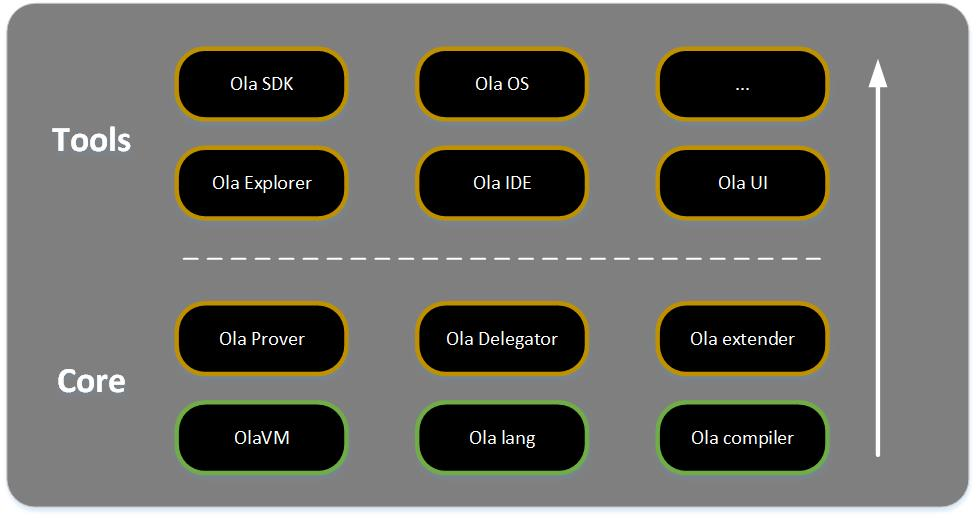
\includegraphics[width=0.6\textwidth]{vm/Ola framework.jpg}
    \caption{Ola framework}
    \label{fig:Ola framework}
\end{figure}

The green borders refers to the modules we have completed implementation, and others stand for the modules we will implement in the future. In the remaining sections of this whitepaper, we will introduce those modules 
as follows:
\begin{itemize}
    \item Section \ref{sec:olavm-a-full-featured-zk-friendly-zkvm} mainly describes the design of Ola's virtual machine, including our zk-friendly design schemes;
    \item Section \ref{sec:ola-lang} mainly describes the design of the customized smart contract language, Ola-lang and the framework of Ola compiler based LLVM;
    \item Section \ref{sec:ola-compiler} mainly describes the design of Ola compiler;
    \item Section \ref{sec:zk-zkvm} mainly describes key points on achieving privacy;
    \item Section \ref{sec:algorithms} mainly describes algorithms used in Ola, including zk and hardware acceleration algorithms;
    \item Section \ref{section:appendix} mainly describes the key features we researched to be supported in the future and our frameworks around that;
    \item Section \ref{sec:glossary} mainly describes some basic notations;
\end{itemize}


    \section{Ola-VM: A Full-featured Zk-friendly ZKVM}\label{sec:olavm-a-full-featured-zk-friendly-zkvm}

\subsection{Design Principles} \label{sec:design-principles}

OlaVM's vision is to build a high-performance, programmable and decentralized Ethernet scaling solution that can help the Ethereum ecosystem to
host more businesses and applications in the future. See \figref{fig:olavm-vision}.
\begin{itemize}
    \item As Layer2, it needs to achieve high performance while taking into account the core features of programmability, composability and
          decentralization, so that existing and future Ethereum applications can be directly deployed on OlaVM;
    \item Higher throughput and lower cost are the demands of these applications
\end{itemize}
You can read \href{https://vitalik.ca/general/2022/09/17/layer_3.html}{Vitalik: What kind of layer 3s make sense?} and
\href{https://medium.com/starkware/fractal-scaling-from-l2-to-l3-7fe238ecfb4f}{Starkware: Fractal Scaling: From L2 to L3} for more discussion
on Layer2, Layer3 features and scenarios.

\begin{figure}[!ht]
    \centering
    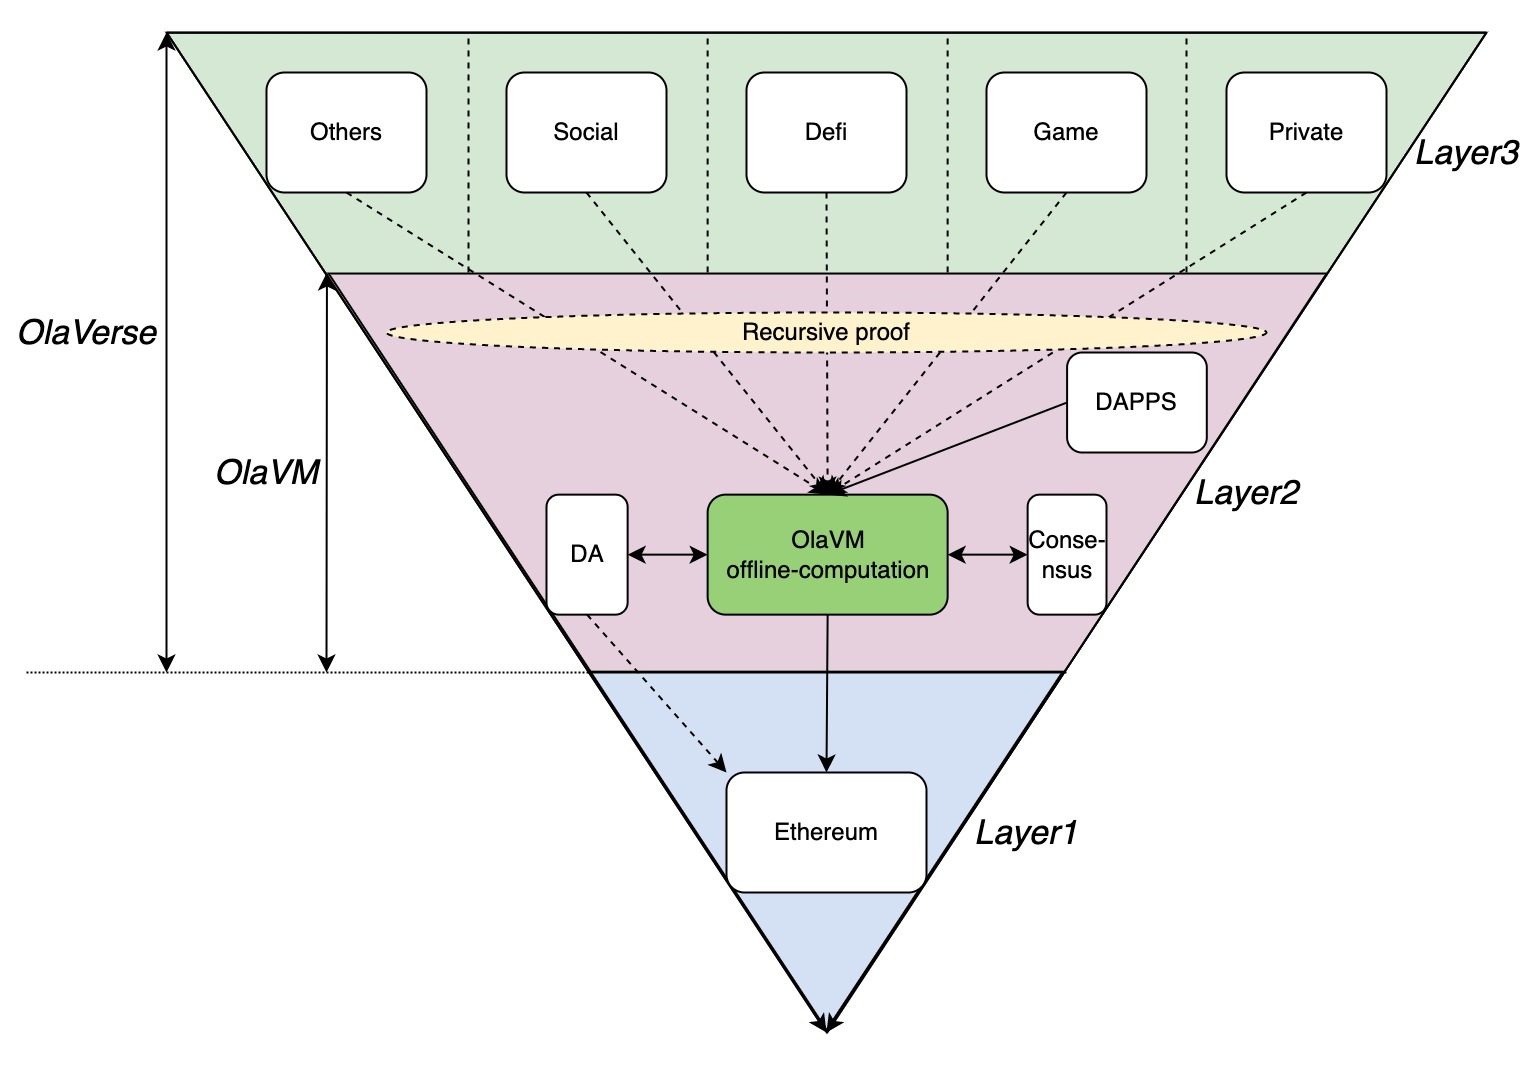
\includegraphics[width=0.8\textwidth]{vm/olavm-vision.jpeg}
    \caption{OlaVM's vision}
    \label{fig:olavm-vision}
\end{figure}

\subsubsection{Design of Instruction Set} \label{sec:design-instruction-set}

OlaVM uses the Reduced Instruction Set Computer (RISC) architecture, one of its main features is a small instruction set, as opposed to the Complex Instruction Set Computer (CISC) architecture.
The difference between the two can be found in \href{https://cs.stanford.edu/people/eroberts/courses/soco/projects/risc/risccisc/}{RISC vs. CISC}.

\emph{1. A reduced instruction set reduces the number of constraint polynomials}

In ZKVM, there is a very critical constraint, the CSTC (CPU State Transition Constraint); it is mainly used to constrain the validity
of VM state changes before and after the execution of an instruction.

\begin{figure}[!ht]
    \centering
    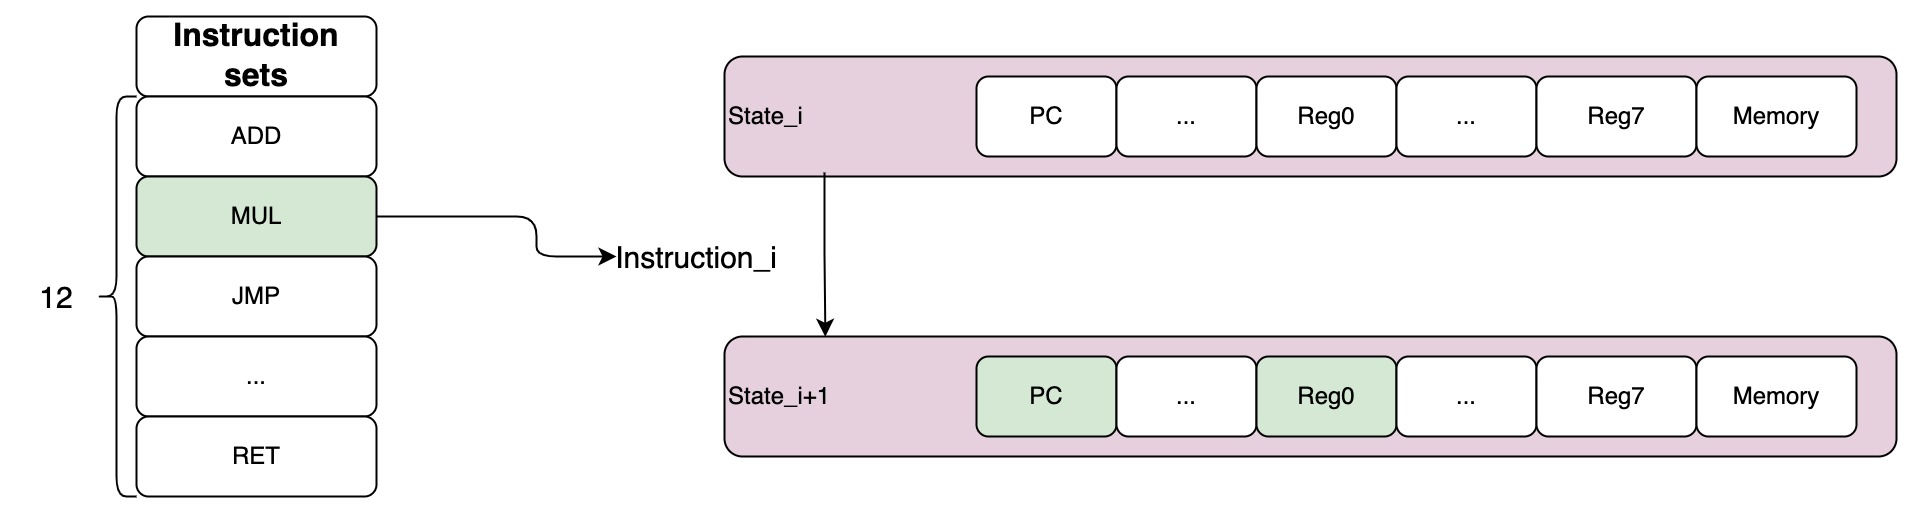
\includegraphics[width=0.7\textwidth]{vm/olavm-instruction-state.jpeg}
    \caption{Instruction-induced cpu state transition}
    \label{fig:instruction-cpu-state-transition}
\end{figure}

As shown in \figref{fig:instruction-cpu-state-transition}, there are many registers in the VM. When VM executes an instruction, it will
cause the state of some registers to change, so to ensure the correctness of VM execution, we need to constrain:
\begin{itemize}
    \item The change of register state involved in the execution of the instruction is valid;
    \item The status of registers not involved in the instruction execution remains unchanged.
\end{itemize}

Let's look at a simple example to explain the constraints on register state changes:
\begin{table}[!ht]
    \centering
    \begin{tabular}{|c|c|c|c|c|c|c|c|}
        \hline
        \rowcolor{gray} clk & pc    & instruction        & \dots & reg0  & reg1  & reg2  & \dots \\
        \hline
        \dots               & \dots & \dots              & \dots & \dots & \dots & \dots & \dots \\
        \hline
        78                  & 8     & ADD reg0 reg0 reg1 & \dots & 1     & 2     & 0     & \dots \\
        \hline
        79                  & 9     & MOV reg2 3         & \dots & 3     & 0     & 0     & \dots \\
        \hline
        80                  & 11    & JMP 2              & \dots & 3     & 0     & 3     & \dots \\
        \hline
        81                  & 2     & \dots              & ...   & 3     & 0     & 3     & \dots \\
        \hline
    \end{tabular}
    \caption{Example of cpu state transitions}
    \label{table:example-cpu-state-transitions}
\end{table}

\tabref{table:example-cpu-state-transitions} briefly presents the changes of some registers after the VM executes three
instructions; taking the PC register as an example, the logic of the updates of the three instructions are:
\begin{itemize}
    \item ADD: $\mathrm{pc}_{i+1} = \mathrm{pc}_i + 1$
    \item MOV: $\mathrm{pc}_{i+1} = \mathrm{pc}_i + 2$
    \item JMP: $\mathrm{pc}_{i+1} = 2$
\end{itemize}

From the point of view of constraints, we do not know which instruction the VM is going to execute each time, so we have to
design a constraint that can handle all instructions, which we call (CSTC) CPU State Transition Constraint.For the simple
example above, we can design the update logic of the PC as follows:
\[ \mathrm{pc}_{i+1} = \mathrm{sel\_jmp}_i \cdot \mathrm{imm\_value} + (1 - \mathrm{sel\_jmp}) \cdot (\mathrm{pc}_i + 1 + \mathrm{op1\_imm}) \]

We write all state transitions of the cpu in this constrained form.The addition of each instruction adds new selectors resulting
in increased constraint complexity, so we limit the size of instructions to 19 (including builtins).

Of course, even though we have a reduced instruction set architecture, we still need to maintain the Turing-complete feature so that
we can still compute everything based on these simple instruction sets.So that based on these simple instruction sets, we can still
compute everything that can be computed. Based on these instructions, combined with the prophet mechanism in Section \ref{sec:design-prophet}, we build a Turing-complete
language, Ola-lang, that supports loops and recursive operations.

\emph{2. Most of the operations will use a small part of the instruction set}

Under the CISC architecture, a large instruction set is defined. However, in reality, each instruction is used differently and for most
of the computations, only a small part of the instruction set may be used.From the constraint point of view, this is a big waste because
the constraint logic of all instructions needs to be included in the constraint system (CSTC), and the worst case would be that each instruction
would correspond to a constraint factor, thus making the whole constraint scale complex, including the number of polynomials and the order of
the constraints.

\begin{figure}[!ht]
    \centering
    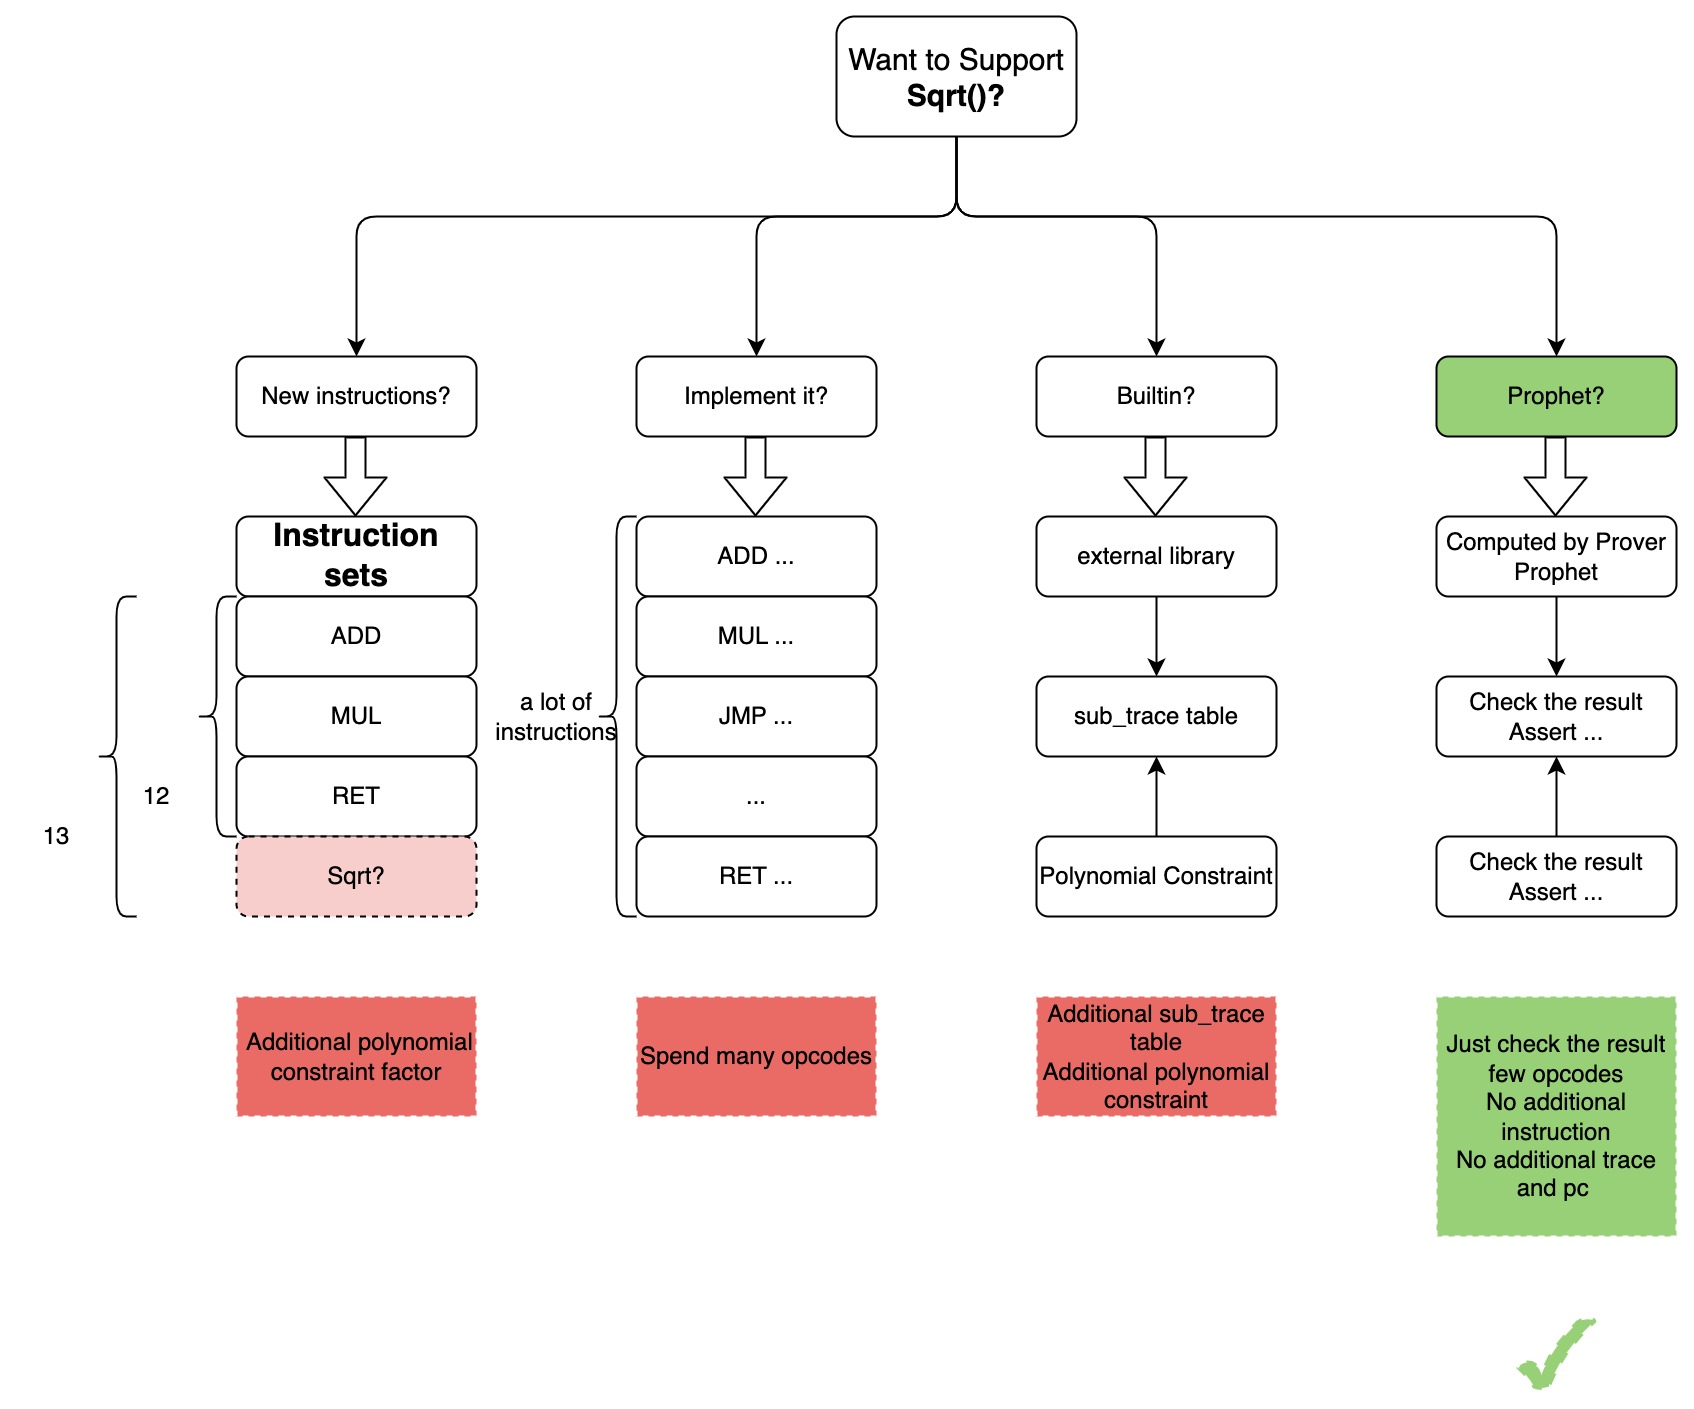
\includegraphics[width=0.6\textwidth]{vm/design-support-zk-unfriendly.jpeg}
    \caption{The best way to support ZK-Unfriendly computation}
    \label{fig:desgin-support-zk-unfriendly}
\end{figure}

For some calculations, in many cases, we prefer to use the existing instruction set rather than introduce a new instruction; 
although this will make the program bigger (more opcodes), some redundant data will be added during the verification itself to
facilitate doing the FFT; but if it is a complex computation that requires a particularly large number of instructions to implement, we still
have ways to solve it, such as introducing Builtins and Prophet, whose principles we will focus on in later chapters, where you just need to
know that they can help drastically reduce the consumption of instructions to implement these complex computations, as shown in \figref{fig:desgin-support-zk-unfriendly}.

\subsubsection{Design of Registers} \label{sec:design-registers}

As mentioned in chapter \ref*{sec:design-instruction-set}, in ZKVM, we not only have to constrain the state of the registers associated with
the instruction to be updated correctly, but we also have to constrain the state of the registers not involved in the current
instruction to remain unchanged.Even though register-based VMs have certain advantages, from the verification point of view,
it is not better to have a larger number of registers;there is a trade-off to be considered:

\begin{itemize}
    \item How many registers will be sufficient for most of the calculations?
    \item For some calculations, is the increased number of memory accesses acceptable when there are not enough registers?
\end{itemize}

If the number of registers is small enough and at the same time the memory accesses introduced do not yet need to be constrained,
this would be the ideal case from the point of view of verification efficiency, as in the design of the Cairo VM, where there are
no general-purpose registers and all operands of the instruction originate from memory;at the same time, to avoid consistency checks
on memory, the write-once model is used, since memory cannot be rewritten at the execution level, so checks are not needed.

However, the downside of introducing the write-once model is that DSLs are not friendly to Dapps developers, and the limitations of
the memory model make it necessary for developers to pay special attention to the way memory is used when developing Dapps with DSLs
(the traditional memory model is the read-write model).

\begin{figure}[!ht]
    \centering
    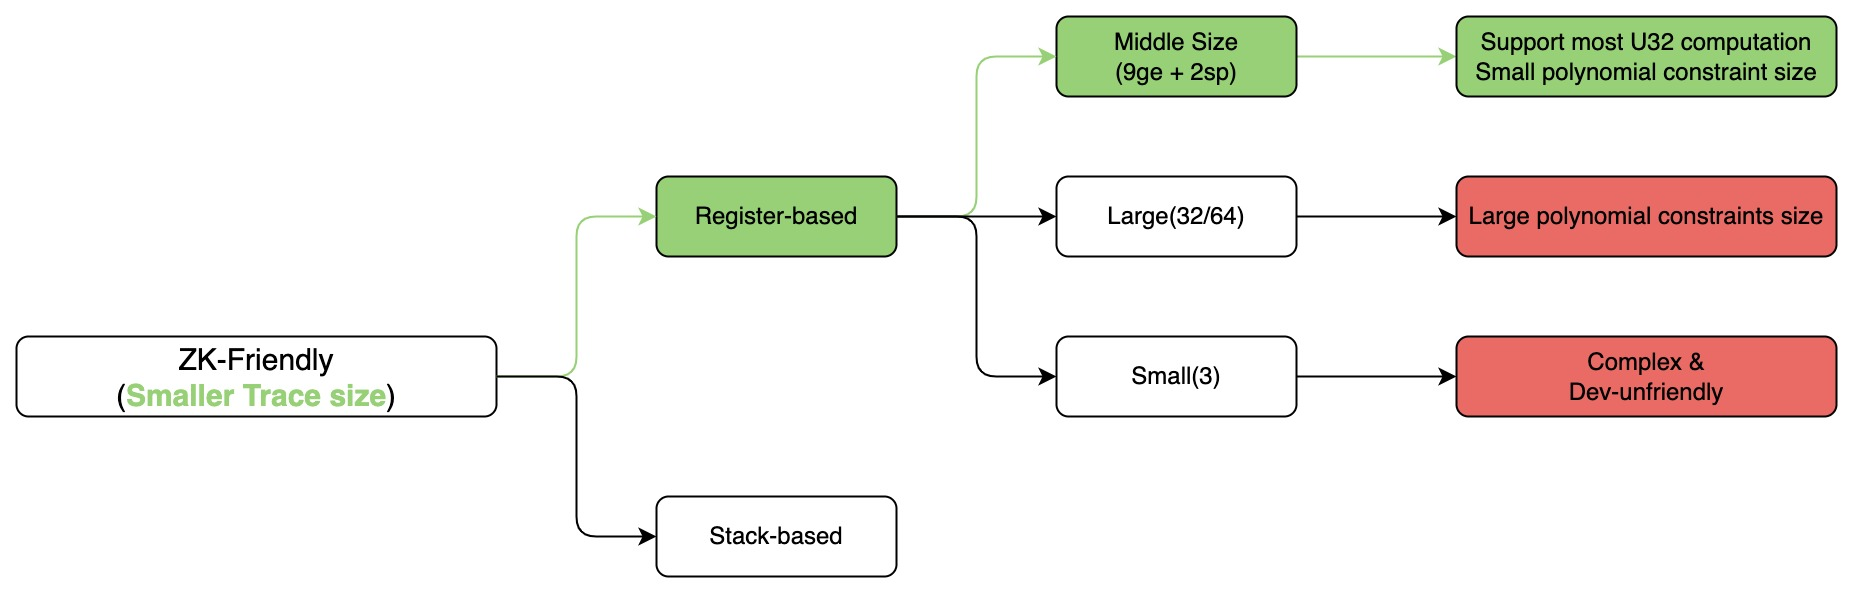
\includegraphics[width=0.8\textwidth]{vm/design-zk-friendly-register.jpeg}
    \caption{How to get ZK-Friendly(Smaller Trace) from register}
    \label{fig:design-zk-friendly-register}
\end{figure}

As shown in \figref{fig:design-zk-friendly-register}, we choose an optimal solution from both ZK-Friendly and Dev-Friendly perspectives.In terms of the number of
registers, considering that the minimum type of computation supported on OlaVM is U32 integer computation, plus some boundary conditions,
such as the number of loops, loop termination conditions, etc, nine general-purpose registers can support most of the U32 computation
(both U64 and U256 integer computation can be implemented through the U32 library), and 2 system registers(PC, PSP) is used in OlaVM, reference: \ref{subsubsec: zkvm-executor-register}. 
When the number of registers is not enough, memory is needed for caching, so memory access-related instructions
(MLOAD, MSTORE) will be added, but it is worth noting that in order to facilitate the FFT, Prover often adds redundant data in Trace to meet
the size of Trace to the power of 2.be replaced with valid data, as shown in \figref{fig:design-better-trace-layout}

\begin{figure}[!ht]
    \centering
    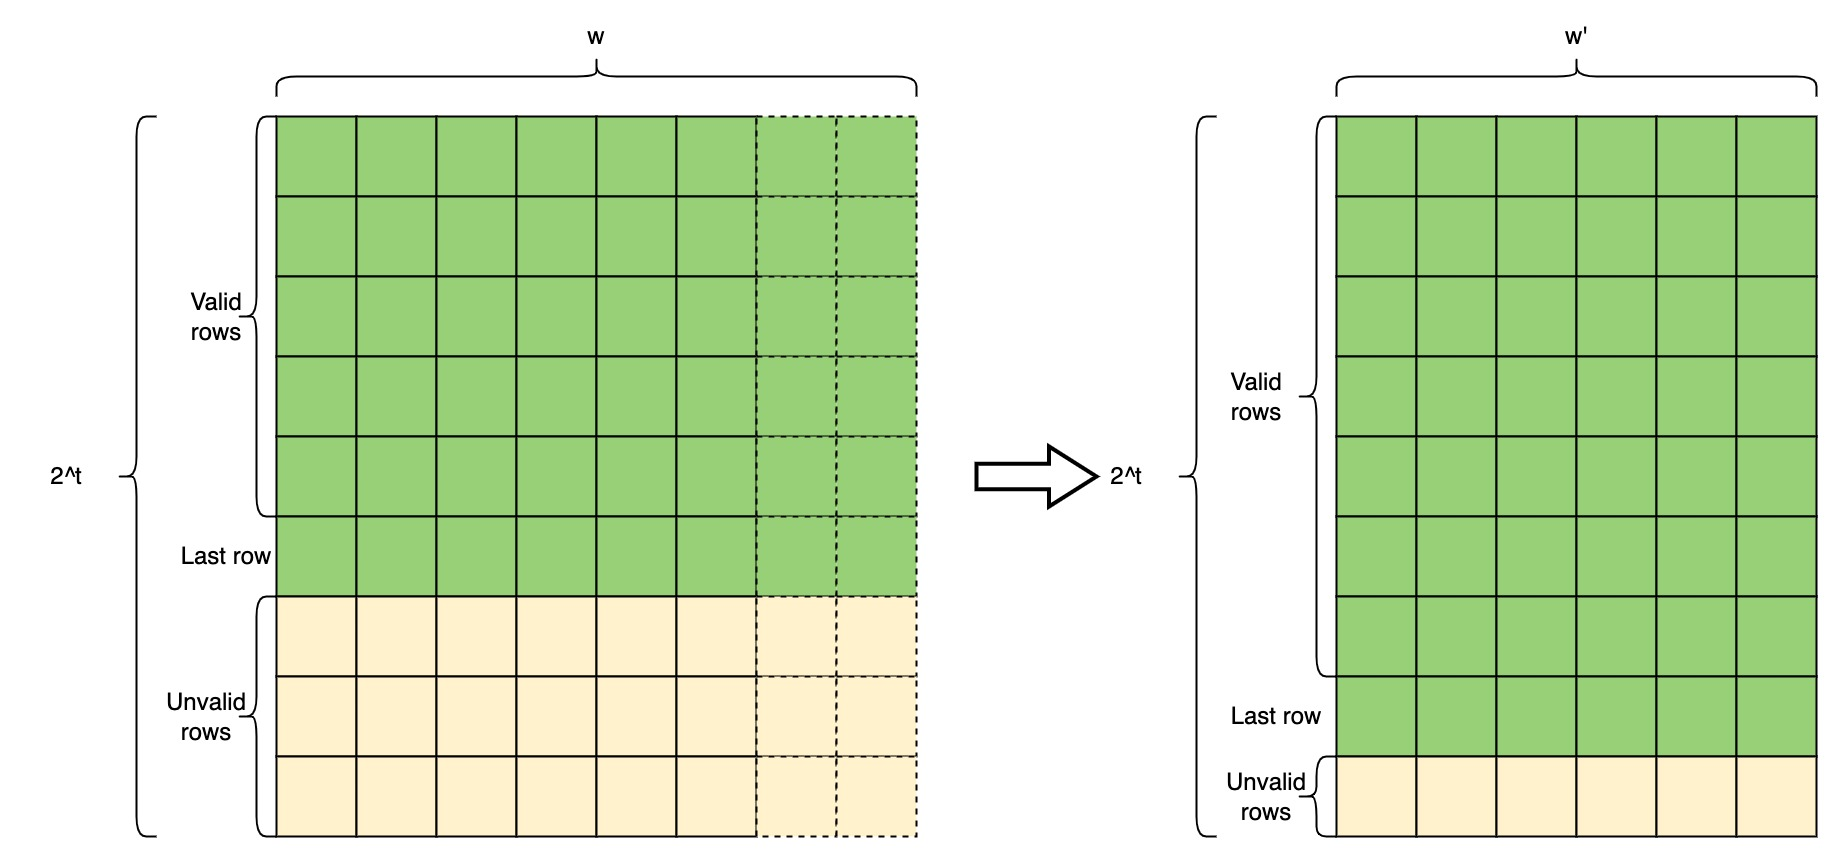
\includegraphics[width=0.8\textwidth]{vm/design-better-trace-layout.jpeg}
    \caption{Better layout of Trace}
    \label{fig:design-better-trace-layout}
\end{figure}
\subsection{Trace Tables} \label{sec:trace-tables}

\subsubsection{Cpu Table} \label{sec:cpu-table}

Context related columns:
\begin{table}[!ht]
    \centering
    \begin{tabular}{|c|c|c|c|c|c|c|c|c|c|c|c|}
        \hline
        clk & pc & reg0 & reg1 & reg2 & reg3 & reg4 & reg5 & reg6 & reg7 & reg8(fp) \\
        \hline
    \end{tabular}
    \caption{Cpu table columns, context related}
    \label{table:cpu-columns-context}
\end{table}

\begin{itemize}
    \item clk: Cpu clock, 1 increment per line.
    \item pc: Program counter, indicates the line number of the currently executed instruction in the program.
    \item reg0 \textasciitilde reg8: Register values. Reg8 may work as general register as well as frame pointer.
\end{itemize}

Instruction related columns:
\begin{table}[!ht]
    \centering
    \begin{tabular}{|c|c|c|c|}
        \hline
        instruction & op1\_imm & opcode & immediate\_value \\
        \hline
    \end{tabular}
    \caption{Cpu table columns, instruction related}
    \label{table:cpu-columns-instruction}
\end{table}

\begin{itemize}
    \item instruction: The currently executing instruction.
    \item op1\_imm: Indicates if op1 is a immediate value.
    \item opcode: The currently executing instruction opcode.
    \item immediate\_value: If current instruction contains immediate value, this should be it.
\end{itemize}

Columns for register selector:
\begin{table}[!ht]
    \centering
    \begin{tabular}{|c|c|c|c|c|c|c|c|c|c|c|c|c|c|}
        \hline
        op0 & op1 & dst & aux0 & aux1 & sel\_op0\_r0 & ... & sel\_op0\_r8 & ... & sel\_op1\_r8 & sel\_dst\_r0 & ... & sel\_dst\_r8 \\
        \hline
    \end{tabular}
    \caption{Cpu table columns for register selector}
    \label{table:cpu-columns-reg-selector}
\end{table}

\begin{itemize}
    \item op0: Value of operand 0, should be a copy of a register.
    \item op1: Value of operand 1, could be a copy of a register or equal to the immediate value.
    \item dst: Value of result, should be a copy of a register.
    \item aux0: Auxillary column, some instruction may use this column.
    \item aux1: Auxillary column, some instruction may use this column.
    \item sel\_op0\_ri: The i-th register is used for op0.
    \item sel\_op1\_ri: The i-th register is used for op1.
    \item sel\_dst\_ri: The i-th register is used for result.
\end{itemize}

Columns for opcode selector:
\begin{table}[!ht]
    \centering
    \begin{tabular}{|c|c|c|c|c|c|c|c|c|c|c|c|}
        \hline
        sel\_add & sel\_mul & sel\_eq & sel\_assert & sel\_mov & sel\_jmp & sel\_cjmp & sel\_call & sel\_ret & sel\_mload & sel\_mstore \\
        \hline
    \end{tabular}
    \caption{Cpu table columns for opcode selector}
    \label{table:cpu-columns-opcode-selector}
\end{table}

\begin{itemize}
    \item sel\_add: Selector for opcode add.
    \item sel\_mul: Selector for opcode mul.
    \item sel\_eq: Selector for opcode eq.
    \item sel\_assert: Selector for opcode assert.
    \item sel\_mov: Selector for opcode mov.
    \item sel\_jmp: Selector for opcode jmp.
    \item sel\_cjmp: Selector for opcode cjmp.
    \item sel\_call: Selector for opcode call.
    \item sel\_ret: Selector for opcode ret.
    \item sel\_mload: Selector for opcode mload.
    \item sel\_mstore: Selector for opcode mstore.
\end{itemize}

Columns for builtin selector:
\begin{table}[!ht]
    \centering
    \begin{tabular}{|c|c|c|c|c|c|c|c|c|}
        \hline
        sel\_range\_check & sel\_and & sel\_or & sel\_xor & sel\_not & sel\_neq & sel\_gte & sel\_poseidon & sel\_ecdsa \\
        \hline
    \end{tabular}
    \caption{Cpu table columns for builtin selector}
    \label{table:cpu-columns-builtin-selector}
\end{table}

\begin{itemize}
    \item sel\_range\_check: Selector for range\_check.
    \item sel\_and: Selector for bitwise and.
    \item sel\_or: Selector for bitwise or.
    \item sel\_xor: Selector for bitwise xor.
    \item sel\_not: Selector for bitwise sel not.
    \item sel\_neq: Selector for comparison neq.
    \item sel\_gte: Selector for comparison gte.
    \item sel\_poseidon: Selector for poseidon hash function.
    \item sel\_ecdsa: Selector for ecdsa.
\end{itemize}
\subsubsection{Memory Table} \label{sec:memory-table}


\begin{table}[!ht]
    \begin{adjustwidth}{-1.75cm}{}
        \setlength{\tabcolsep}{2pt}
        \centering
        \begin{tabular}{|c|c|c|c|c|c|c|c|c|c|c|c|c|c|c|c|c|}
            \hline
            \rowcolor{gray} is\_rw     & addr   & clk   & opcode & is\_write & value & diff\_addr                     & \makecell{diff\_                                                                                                                                                                                                        \\addr\_inv} & diff\_clk & \makecell{diff\_add\\r\_cond} & \makecell{filter\_looked\\\_for\_main} & \makecell{rv\_addr\\\_unchanged} & \makecell{region\\\_prophet} & \makecell{region\\\_poseidon} & \makecell{region\\\_ecdsa} & rc\_value & \makecell{filter\_\\looking\_rc} \\
            \hline
            \rowcolor{green!20} 1      & 100    & 5     & mstore & 1         & 55    & \cellcolor{lightgray} 0        & \cellcolor{lightgray} 0     & \cellcolor{lightgray} 0     & \cellcolor{lightgray} 0 & \cellcolor{violet!30} 1     & 0     & \cellcolor{pink} 0     & \cellcolor{pink} 0     & \cellcolor{pink} 0     & 0        & 1     \\
            \hline
            \rowcolor{green!20} 1      & 100    & 12    & mload  & 0         & 55    & 0                              & 0                           & 7                           & \cellcolor{lightgray} 0 & \cellcolor{violet!30} 1     & 1     & \cellcolor{pink} 0     & \cellcolor{pink} 0     & \cellcolor{pink} 0     & 7        & 1     \\
            \hline
            \rowcolor{green!20} 1      & 100    & 17    & mstore & 1         & 300   & 0                              & 0                           & 5                           & \cellcolor{lightgray} 0 & \cellcolor{violet!30} 1     & 1     & \cellcolor{pink} 0     & \cellcolor{pink} 0     & \cellcolor{pink} 0     & 5        & 1     \\
            \hline
            \rowcolor{green!20} 1      & 100    & 26    & mload  & 0         & 300   & 0                              & 0                           & 9                           & \cellcolor{lightgray} 0 & \cellcolor{violet!30} 1     & 1     & \cellcolor{pink} 0     & \cellcolor{pink} 0     & \cellcolor{pink} 0     & 9        & 1     \\
            \hline
            \rowcolor{green!20} 1      & 124    & 36    & mstore & 1         & 20000 & 24                             & (1/24)                      & \cellcolor{lightgray} 0     & \cellcolor{lightgray} 0 & \cellcolor{violet!30} 1     & 0     & \cellcolor{pink} 0     & \cellcolor{pink} 0     & \cellcolor{pink} 0     & 24       & 1     \\
            \hline
            \rowcolor{green!20} 1      & 124    & 37    & call   & 0         & 20000 & 0                              & 0                           & 1                           & \cellcolor{lightgray} 0 & \cellcolor{violet!30} 1     & 1     & \cellcolor{pink} 0     & \cellcolor{pink} 0     & \cellcolor{pink} 0     & 1        & 1     \\
            \hline
            \rowcolor{green!20} 1      & 124    & 50    & ret    & 0         & 20000 & 0                              & 0                           & 13                          & \cellcolor{lightgray} 0 & \cellcolor{violet!30} 1     & 1     & \cellcolor{pink} 0     & \cellcolor{pink} 0     & \cellcolor{pink} 0     & 13       & 1     \\
            \hline
            \rowcolor{green!20} 1      & 125    & 37    & call   & 1         & 30000 & 1                              & 1                           & \cellcolor{lightgray} 0     & \cellcolor{lightgray} 0 & \cellcolor{violet!30} 1     & 0     & \cellcolor{pink} 0     & \cellcolor{pink} 0     & \cellcolor{pink} 0     & 1        & 1     \\
            \hline
            \rowcolor{green!20} 1      & 125    & 50    & ret    & 0         & 30000 & 0                              & 0                           & 13                          & \cellcolor{lightgray} 0 & \cellcolor{violet!30} 1     & 1     & \cellcolor{pink} 0     & \cellcolor{pink} 0     & \cellcolor{pink} 0     & 13       & 1     \\
            \hline
            \rowcolor{green!20} 1      & 150    & 20    & mstore & 1         & 78    & 25                             & (1/25)                      & \cellcolor{lightgray} 0     & \cellcolor{lightgray} 0 & \cellcolor{violet!30} 1     & 0     & \cellcolor{pink} 0     & \cellcolor{pink} 0     & \cellcolor{pink} 0     & 25       & 1     \\
            \hline
            \rowcolor{green!20} 1      & 150    & 23    & mload  & 0         & 78    & 0                              & 0                           & 3                           & \cellcolor{lightgray} 0 & \cellcolor{violet!30} 1     & 1     & \cellcolor{pink} 0     & \cellcolor{pink} 0     & \cellcolor{pink} 0     & 3        & 1     \\
            \hline
            \rowcolor{green!20} 1      & 200    & 8     & mstore & 1         & 99    & 50                             & (1/50)                      & \cellcolor{lightgray} 0     & \cellcolor{lightgray} 0 & \cellcolor{violet!30} 1     & 0     & \cellcolor{pink} 0     & \cellcolor{pink} 0     & \cellcolor{pink} 0     & 50       & 1     \\
            \hline
            \rowcolor{green!20} 1      & 200    & 15    & mload  & 0         & 99    & 0                              & 0                           & 7                           & \cellcolor{lightgray} 0 & \cellcolor{violet!30} 1     & 1     & \cellcolor{pink} 0     & \cellcolor{pink} 0     & \cellcolor{pink} 0     & 7        & 1     \\
            \hline
            \rowcolor{yellow!20} 0     & p'''   & 0     & 0      & 1         & in    & \cellcolor{lightgray} p'''-200 & \cellcolor{lightgray} 0     & \cellcolor{lightgray} 0     & p''-addr                & \cellcolor{violet!30} 0     & 0     & \cellcolor{pink} 0     & \cellcolor{pink} 0     & \cellcolor{pink} 1     & p''-addr & 1     \\
            \hline
            \rowcolor{yellow!20} 0     & p'''+1 & 0     & 0      & 1         & in    & \cellcolor{lightgray} 1        & \cellcolor{lightgray} 0     & \cellcolor{lightgray} 0     & p''-addr                & \cellcolor{violet!30} 0     & 0     & \cellcolor{pink} 0     & \cellcolor{pink} 0     & \cellcolor{pink} 1     & p''-addr & 1     \\
            \hline
            \rowcolor{yellow!20} 0     & p'''+2 & 0     & 0      & 1         & out   & \cellcolor{lightgray} 1        & \cellcolor{lightgray} 0     & \cellcolor{lightgray} 0     & p''-addr                & \cellcolor{violet!30} 0     & 0     & \cellcolor{pink} 0     & \cellcolor{pink} 0     & \cellcolor{pink} 1     & p''-addr & 1     \\
            \hline
            \rowcolor{yellow!20} 0     & p'''+2 & 44    & mload  & 0         & out   & \cellcolor{lightgray} 0        & \cellcolor{lightgray} 0     & \cellcolor{lightgray} 0     & p''-addr                & \cellcolor{violet!30} 1     & 0     & \cellcolor{pink} 0     & \cellcolor{pink} 0     & \cellcolor{pink} 1     & p''-addr & 1     \\
            \hline
            \rowcolor{yellow!20} 0     & p'''+3 & 0     & 0      & 1         & out   & \cellcolor{lightgray} 1        & \cellcolor{lightgray} 0     & \cellcolor{lightgray} 0     & p''-addr                & \cellcolor{violet!30} 0     & 0     & \cellcolor{pink} 0     & \cellcolor{pink} 0     & \cellcolor{pink} 1     & p''-addr & 1     \\
            \hline
            \rowcolor{yellow!20} 0     & p'''+3 & 45    & mload  & 0         & out   & \cellcolor{lightgray} 0        & \cellcolor{lightgray} 0     & \cellcolor{lightgray} 0     & p''-addr                & \cellcolor{violet!30} 1     & 0     & \cellcolor{pink} 0     & \cellcolor{pink} 0     & \cellcolor{pink} 1     & p''-addr & 1     \\
            \hline
            \rowcolor{yellow!20} \dots & \dots  & \dots & \dots  & \dots     & \dots & \cellcolor{lightgray} \dots    & \cellcolor{lightgray} \dots & \cellcolor{lightgray} \dots & \dots                   & \cellcolor{violet!30} \dots & \dots & \cellcolor{pink} \dots & \cellcolor{pink} \dots & \cellcolor{pink} \dots & \dots    & \dots \\
            \hline
            \rowcolor{yellow!20} 0     & p''    & 0     & 0      & 1         & in    & \cellcolor{lightgray} \dots    & \cellcolor{lightgray} 0     & \cellcolor{lightgray} 0     & p'-addr                 & \cellcolor{violet!30} 0     & 0     & \cellcolor{pink} 0     & \cellcolor{pink} 1     & \cellcolor{pink} 0     & p'-addr  & 1     \\
            \hline
            \rowcolor{yellow!20} 0     & p''+1  & 0     & 0      & 1         & in    & \cellcolor{lightgray} 1        & \cellcolor{lightgray} 0     & \cellcolor{lightgray} 0     & p'-addr                 & \cellcolor{violet!30} 0     & 0     & \cellcolor{pink} 0     & \cellcolor{pink} 1     & \cellcolor{pink} 0     & p'-addr  & 1     \\
            \hline
            \rowcolor{yellow!20} 0     & p''+2  & 0     & 0      & 1         & out   & \cellcolor{lightgray} 1        & \cellcolor{lightgray} 0     & \cellcolor{lightgray} 0     & p'-addr                 & \cellcolor{violet!30} 0     & 0     & \cellcolor{pink} 0     & \cellcolor{pink} 1     & \cellcolor{pink} 0     & p'-addr  & 1     \\
            \hline
            \rowcolor{yellow!20} 0     & p''+2  & 55    & mload  & 0         & out   & \cellcolor{lightgray} 0        & \cellcolor{lightgray} 0     & \cellcolor{lightgray} 0     & p'-addr                 & \cellcolor{violet!30} 1     & 0     & \cellcolor{pink} 0     & \cellcolor{pink} 1     & \cellcolor{pink} 0     & p'-addr  & 1     \\
            \hline
            \rowcolor{yellow!20} 0     & p''+3  & 0     & 0      & 1         & out   & \cellcolor{lightgray} 1        & \cellcolor{lightgray} 0     & \cellcolor{lightgray} 0     & p'-addr                 & \cellcolor{violet!30} 0     & 0     & \cellcolor{pink} 0     & \cellcolor{pink} 1     & \cellcolor{pink} 0     & p'-addr  & 1     \\
            \hline
            \rowcolor{yellow!20} 0     & p''+3  & 56    & mload  & 0         & out   & \cellcolor{lightgray} 0        & \cellcolor{lightgray} 0     & \cellcolor{lightgray} 0     & p'-addr                 & \cellcolor{violet!30} 1     & 0     & \cellcolor{pink} 0     & \cellcolor{pink} 1     & \cellcolor{pink} 0     & p'-addr  & 1     \\
            \hline
            \rowcolor{yellow!20} \dots & \dots  & \dots & \dots  & \dots     & \dots & \cellcolor{lightgray} \dots    & \cellcolor{lightgray} \dots & \cellcolor{lightgray} \dots & \dots                   & \cellcolor{violet!30} \dots & \dots & \cellcolor{pink} \dots & \cellcolor{pink} \dots & \cellcolor{pink} \dots & \dots    & \dots \\
            \hline
            \rowcolor{yellow!20} 0     & p'     & 0     & 0      & 1         & 123   & \cellcolor{lightgray} \dots    & \cellcolor{lightgray} 0     & \cellcolor{lightgray} 0     & p-addr                  & \cellcolor{violet!30} 0     & 0     & \cellcolor{pink} 1     & \cellcolor{pink} 0     & \cellcolor{pink} 0     & p-addr   & 1     \\
            \hline
            \rowcolor{yellow!20} 0     & p'     & 7     & mload  & 0         & 123   & \cellcolor{lightgray} 0        & \cellcolor{lightgray} 0     & \cellcolor{lightgray} 0     & p-addr                  & \cellcolor{violet!30} 1     & 0     & \cellcolor{pink} 1     & \cellcolor{pink} 0     & \cellcolor{pink} 0     & p-addr   & 1     \\
            \hline
            \rowcolor{yellow!20} 0     & p'     & 9     & mload  & 0         & 123   & \cellcolor{lightgray} 0        & \cellcolor{lightgray} 0     & \cellcolor{lightgray} 0     & p-addr                  & \cellcolor{violet!30} 1     & 0     & \cellcolor{pink} 1     & \cellcolor{pink} 0     & \cellcolor{pink} 0     & p-addr   & 1     \\
            \hline
            \rowcolor{yellow!20} 0     & p'+1   & 0     & 0      & 1         & 456   & \cellcolor{lightgray} 1        & \cellcolor{lightgray} 0     & \cellcolor{lightgray} 0     & p-addr                  & \cellcolor{violet!30} 0     & 0     & \cellcolor{pink} 1     & \cellcolor{pink} 0     & \cellcolor{pink} 0     & p-addr   & 1     \\
            \hline
            \rowcolor{yellow!20} 0     & p'+1   & 27    & mload  & 0         & 456   & \cellcolor{lightgray} 0        & \cellcolor{lightgray} 0     & \cellcolor{lightgray} 0     & p-addr                  & \cellcolor{violet!30} 1     & 0     & \cellcolor{pink} 1     & \cellcolor{pink} 0     & \cellcolor{pink} 0     & p-addr   & 1     \\
            \hline
        \end{tabular}
        \caption{Memory Trace Table}
        \label{table:memory-trace-table}
    \end{adjustwidth}
\end{table}

\begin{itemize}
    \item is\_rw: Indicates whether the current memory is in read-write segment.
    \item addr: Address of memory.
    \item clk: Clock when access memory this time.
    \item opcode: The opcode that triggered this memory access.In write-once segment, no corresponding opcode for write access, and should be 0 here.
    \item is\_write: Indicates whether this memory access is write.
    \item value: Value in the memory cell.
    \item diff\_addr: Address difference between two rows.
    \item diff\_addr\_inv: The reciprocal of the address difference between the two rows.Only used in read-write segment, in write-once segment, should be 0.
    \item diff\_clk: Clock difference between two rows.Only used in read-write segment, in write-once segment, should be 0.
    \item diff\_addr\_cond:
          \begin{itemize}
              \item Read-write segment: Should be 0 here.
              \item Ecdsa segment: p'' - addr.
              \item Poseidon segment: p' - addr.
              \item Prophet segment: p - addr.
          \end{itemize}
    \item filter\_looked\_for\_main: Filter column for cross table lookup between cpu table and memory table, should be 0 when opcode is 0 and 1 otherwise.
    \item rw\_addr\_unchanged: Indicates current address is in read-write segment, and address is the same as the last row.
    \item region\_prophet: Indicates current address is in prophet segment.
    \item region\_poseidon: Indicates current address is in poseidon segment.
    \item region\_ecdsa: Indicates current address is in ecdsa segment.
    \item rc\_value: Value used for range check.
          \begin{itemize}
              \item  Read-write segment: Should be diff\_clk(addr not changed) or diff\_addr(addr changed).
              \item Write-once segments: Should be diff\_addr\_cond.
          \end{itemize}
    \item filter\_looking\_rc: Filter column for cross table lookup between memory table and range-check table, should all be 1.
\end{itemize}
\subsubsection{Builtin Tables} \label{sec:builtin-tables}

\subsubsubsection{Range check Table} \label{sec:range-check-table}
\begin{table}[!ht]
    \centering
    \begin{tabular}{|c|c|c|c|c|c|}
        \hline
        \rowcolor{gray} filter\_looked\_for\_cpu & filter\_looked\_for\_memory & filter\_looked\_for\_cmp & val        & limb\_lo & limb\_high \\
        \hline
        1                                        & 0                           & 0                        & 0xffff0000 & 0x0      & 0xffff     \\
        \hline
        0                                        & 1                           & 0                        & 0x1        & 0x0      & 0x1        \\
        \hline
        0                                        & 0                           & 1                        & 0xe00a0    & 0xe      & 0xa0       \\
        \hline
    \end{tabular}
    \caption{Range Check Table}
    \label{table:range-check-table}
\end{table}
\begin{itemize}
    \item filter\_looked\_for\_cpu: Filter column for cross table lookup between cpu table and range-check table.
    \item filter\_looked\_for\_memory: Filter column for cross table lookup between memory table and range-check table.
    \item filter\_looked\_for\_cmp: Filter column for cross table lookup between comparison table and range-check table.
    \item val: Value to be range checked.
    \item limb\_lo: Low 16 bits of val.
    \item limb\_high: Hight 16 bits of val.
\end{itemize}

In addition to these columns, there are also columns for fixed table lookup including: limb\_lo\_permuted, limb\_hi\_permuted, fix\_rc\_u16, fix\_rc\_permuted\_lo, fix\_rc\_permuted\_hi.

\subsubsubsection{Comparison Table} \label{sec:comparison-table}
\begin{table}[!ht]
    \centering
    \begin{tabular}{|c|c|c|c|c|c|}
        \hline
        \rowcolor{gray} op0 & op1 & gte & abs\_diff & abs\_diff\_inv & filter\_looking\_rc \\
        \hline
        5                   & 3   & 1   & 2         & (1/2)          & 1                   \\
        \hline
        2                   & 7   & 0   & 5         & (1/5)          & 1                   \\
        \hline
        6                   & 6   & 1   & 0         & 0              & 1                   \\
        \hline
    \end{tabular}
    \caption{Comparison Table}
    \label{table:comparison-table}
\end{table}
\begin{itemize}
    \item op0: Comparison first operand.
    \item op1: Comparison second operand.
    \item gte: Indicates whether this row is constrained for gte or lt.
    \item abs\_diff: Absolute value of the difference between two operands.
    \item abs\_diff\_inv: The reciprocal of abs\_diff.
    \item fliter\_looking\_rc: Filter column for cross table lookup between comparison table and range-check table.
\end{itemize}

\subsubsubsection{Bitwise Table} \label{sec:bitwise-table}
\begin{table}[!ht]
    \centering
    \begin{adjustwidth}{-1cm}{}
        \begin{tabular}{|c|c|c|c|c|c|c|c|c|c|c|c|c|c|c|c|}
            \hline
            \rowcolor{gray} opcode & op0 & op1 & res & op0\_0 & op0\_1 & op0\_2 & op0\_3 & op1\_0 & op1\_1 & op1\_2 & op1\_3 & res\_0 & res\_1 & res\_2 & res\_3 \\
            \hline
            and                    & 30  & 10  & 10  & 30     & 0      & 0      & 0      & 10     & 0      & 0      & 0      & 10     & 0      & 0      & 0      \\
            \hline
            or                     & 2   & 30  & 30  & 2      & 0      & 0      & 0      & 30     & 0      & 0      & 0      & 30     & 0      & 0      & 0      \\
            \hline
            xor                    & 10  & 3   & 9   & 10     & 0      & 0      & 0      & 3      & 0      & 0      & 0      & 9      & 0      & 0      & 0      \\
            \hline
        \end{tabular}
    \end{adjustwidth}
    \caption{Bitwise Table}
    \label{table:bitwise-table}
\end{table}
\begin{itemize}
    \item opcode: Can be and/or/xor.
    \item op0: Bitwise first operand.
    \item op1: Bitwise second operand.
    \item res: Bitwise result.
    \item op0\_i: i-th limb of op0.
    \item op1\_i: i-th limb of op1.
    \item res\_i: i-th limb of res.
\end{itemize}

In addition to these columns, there are also some columns used for fixed table lookup.
\subsection{Constraints} \label{sec:constraints}

\subsubsection{Constraints for Cpu Table} \label{sec:cpu-constraints}

\emph{Instruction encode related constraints}

Related columns include: instruction, opcode, op\_imm, sel\_opi\_rj and opcode/builtins selector columns.

op\_imm should be binary:
\[ \mathrm{op\_imm}_i * (1 - \mathrm{op\_imm}_i) = 0 \]

Selectors should be binary:
\[ \mathrm{sel\_op0\_r0}_i \cdot (1-\mathrm{sel\_op0\_r0}_i) = 0 \]
\[ \mathrm{sel\_op0\_r1}_i \cdot (1-\mathrm{sel\_op0\_r1}_i) = 0 \]
\dots
\[ \mathrm{sel\_op0\_r8}_i \cdot (1-\mathrm{sel\_op0\_r8}_i) = 0 \]
\[ \mathrm{sel\_op1\_r0}_i \cdot (1-\mathrm{sel\_op1\_r0}_i) = 0 \]
\[ \mathrm{sel\_op1\_r1}_i \cdot (1-\mathrm{sel\_op1\_r1}_i) = 0 \]
\[ \mathrm{sel\_op1\_r2}_i \cdot (1-\mathrm{sel\_op1\_r2}_i) = 0 \]
\dots
\[ \mathrm{sel\_op1\_r8}_i \cdot (1-\mathrm{sel\_op1\_r8}_i) = 0 \]
\[ \mathrm{sel\_dst\_r0}_i \cdot (1-\mathrm{sel\_dst\_r0}_i) = 0 \]
\[ \mathrm{sel\_dst\_r1}_i \cdot (1-\mathrm{sel\_dst\_r1}_i) = 0 \]
\dots
\[ \mathrm{sel\_dst\_r8}_i \cdot (1-\mathrm{sel\_dst\_r8}_i) = 0 \]
\[ \mathrm{sel\_add}_i \cdot (1-\mathrm{sel\_add}_i) = 0 \]
\[ \mathrm{sel\_mul}_i \cdot (1-\mathrm{sel\_mul}_i) = 0 \]
\[ \mathrm{sel\_eq} \cdot (1-\mathrm{sel\_eq}_i) = 0 \]
\[ \mathrm{sel\_assert}_i \cdot (1-\mathrm{sel\_assert}_i) = 0 \]
\[ \mathrm{sel\_mov}_i \cdot (1 - \mathrm{sel\_mov}_i) = 0 \]
\[ \mathrm{sel\_jmp}_i \cdot (1 - \mathrm{sel\_jmp}_i) = 0 \]
\[ \mathrm{sel\_cjmp}_i \cdot (1 - \mathrm{sel\_cjmp}_i) = 0 \]
\[ \mathrm{sel\_call}_i \cdot (1 - \mathrm{sel\_call}_i) = 0 \]
\[ \mathrm{sel\_ret}_i \cdot (1 - \mathrm{sel\_ret}_i) = 0 \]
\[ \mathrm{sel\_mload} \cdot (1 - \mathrm{sel\_mload}_i) = 0 \]
\[ \mathrm{sel\_mstore}_i \cdot (1 - \mathrm{sel\_mstore}_i) = 0 \]
\[ \mathrm{sel\_end}_i  \cdot (1 - \mathrm{sel\_end}_i) = 0 \]
\[ \mathrm{sel\_range\_check}_i \cdot (1 - \mathrm{sel\_range\_check}_i) = 0 \]
\[ \mathrm{sel\_and}_i \cdot (1 - \mathrm{sel\_and}_i) = 0 \]
\[ \mathrm{sel\_or}_i \cdot (1 - \mathrm{sel\_or}_i) = 0 \]
\[ \mathrm{sel\_xor}_i \cdot (1 - \mathrm{sel\_xor}_i) = 0 \]
\[ \mathrm{sel\_not}_i \cdot (1 - \mathrm{sel\_not}_i) = 0 \]
\[ \mathrm{sel\_neq}_i \cdot (1 - \mathrm{sel\_neq}_i) = 0 \]
\[ \mathrm{sel\_gte}_i \cdot (1 - \mathrm{sel\_gte}_i) = 0 \]
\[ \mathrm{sel\_poseidon}_i \cdot (1 - \mathrm{sel\_poseidon}_i) = 0 \]
\[ \mathrm{sel\_ecdsa}_i \cdot (1 - \mathrm{sel\_ecdsa}_i) = 0 \]

Opcode encode constraint:
\begin{multline*}
    \mathrm{opcode}_i - (\mathrm{sel\_add}_i \cdot 2^{34} + \mathrm{sel\_mul}_i \cdot 2^{33} + \mathrm{sel\_eq} \cdot 2^{32} + \mathrm{sel\_assert}_i \cdot 2^{31} + \mathrm{sel\_mov}_i \cdot 2^{30} + \mathrm{sel\_jmp}_i \cdot 2^{29} \\
    + \mathrm{sel\_cjmp}_i \cdot 2^{28} + \mathrm{sel\_call}_i \cdot 2^{27} + \mathrm{sel\_ret}_i \cdot 2^{26} + \mathrm{sel\_mload} \cdot 2^{25} + \mathrm{sel\_mstore}_i \cdot 2^{24} \\
    + \mathrm{sel\_end}_i  \cdot 2^{23} + \mathrm{sel\_range\_check}_i \cdot 2^{22} + \mathrm{sel\_and}_i \cdot 2^{21} + \mathrm{sel\_or}_i \cdot 2^{20} + \mathrm{sel\_xor}_i \cdot 2^{19} \\
    + \mathrm{sel\_not}_i \cdot 2^{18} + \mathrm{sel\_neq}_i \cdot 2^{17} + \mathrm{sel\_gte}_i \cdot 2^{16} + \mathrm{sel\_poseidon}_i \cdot 2^{15} + \mathrm{sel\_ecdsa}_i \cdot 2^{14}) = 0
\end{multline*}

Instruction encode constraint:
\begin{multline*}
    \mathrm{instruction}_i - (\mathrm{op1\_imm}_i \cdot 2^{62} + \mathrm{sel\_op0\_r8}_i \cdot 2^{61} + \mathrm{sel\_op0\_r7}_i \cdot 2^{60} + \mathrm{sel\_op0\_r6}_i \cdot 2^{59} + \mathrm{sel\_op0\_r5}_i \cdot 2^{58} \\
    + \mathrm{sel\_op0\_r4}_i \cdot 2^{57} + \mathrm{sel\_op0\_r3}_i \cdot 2^{56} + \mathrm{sel\_op0\_r2}_i \cdot 2^{55} + \mathrm{sel\_op0\_r1}_i \cdot 2^{54} + \mathrm{sel\_op0\_r0}_i \cdot 2^{53} \\
    + \mathrm{sel\_op1\_r8}_i \cdot 2^{52} + \mathrm{sel\_op1\_r7}_i \cdot 2^{51} + \mathrm{sel\_op1\_r6}_i \cdot 2^{50} + \mathrm{sel\_op1\_r5}_i \cdot 2^{49} + \mathrm{sel\_op1\_r4}_i \cdot 2^{48} \\
    + \mathrm{sel\_op1\_r3}_i \cdot 2^{47} + \mathrm{sel\_op1\_r2}_i \cdot 2^{46} + \mathrm{sel\_op1\_r1}_i \cdot 2^{45} + \mathrm{sel\_op1\_r0}_i \cdot 2^{44} + \mathrm{sel\_dst\_r8}_i \cdot 2^{43} \\
    + \mathrm{sel\_dst\_r7}_i \cdot 2^{42} + \mathrm{sel\_dst\_r6}_i \cdot 2^{41} + \mathrm{sel\_dst\_r5}_i \cdot 2^{40} + \mathrm{sel\_dst\_r4}_i \cdot 2^{39} + \mathrm{sel\_dst\_r3}_i \cdot 2^{38} \\
    + \mathrm{sel\_dst\_r2}_i \cdot 2^{37} + \mathrm{sel\_dst\_r1}_i \cdot 2^{36} + \mathrm{sel\_dst\_r0}_i \cdot 2^{35} + \mathrm{opcode}_i) = 0
\end{multline*}

\emph{Operands and their selector constraints}

Define the following virtual columns:
\[ \widetilde{\mathrm{enable\_op0}}_i=\sum_{x=0}^8 \mathrm{sel\_op0\_rx}_i \]
\[ \widetilde{\mathrm{enable\_op0}}_i=\sum_{x=0}^8 \mathrm{sel\_op0\_rx}_i \]
\[ \widetilde{\mathrm{enable\_op0}}_i=\sum_{x=0}^8 \mathrm{sel\_op0\_rx}_i \]

Register selector constraints:
\[ \widetilde{\mathrm{enable\_op0}}_i \cdot (1-\widetilde{\mathrm{enable\_op0}}_i)=0 \]
\[ \widetilde{\mathrm{enable\_op1}}_i \cdot (1-\widetilde{\mathrm{enable\_op1}}_i)=0 \]
\[ \widetilde{\mathrm{enable\_dst}}_i \cdot (1-\widetilde{\mathrm{enable\_dst}}_i)=0 \]

Copy constraints between and related register:
\[ \widetilde{\mathrm{enable\_op0}}_i \cdot (\mathrm{op0}_i-\sum_{x=0}^8 \mathrm{sel\_op0\_rx}_i \cdot \mathrm{regx}_i)=0 \]
\[ \widetilde{\mathrm{enable\_op1}}_i \cdot (\mathrm{op1}_i-\sum_{x=0}^8 \mathrm{sel\_op1\_rx}_i \cdot \mathrm{regx}_i)=0 \]
\[ \widetilde{\mathrm{enable\_dst}}_i \cdot (\mathrm{dst}_i-\sum_{x=0}^8 \mathrm{sel\_dst\_rx}_i \cdot \mathrm{regx}_{i+1})=0 \]

If op1\_imm is 1, then op1 equals the immediate value:
\[ \mathrm{op1\_imm}_i \cdot (\mathrm{op1}_i - \mathrm{immediate\_value}_i)=0 \]

Only one operation selector can be enabled at a time:
\begin{multline*}
    1 - (\mathrm{sel\_add}_i + \mathrm{sel\_mult}_i + \mathrm{sel\_eq}_i + \mathrm{sel\_assert}_i + \mathrm{sel\_mov}_i + \mathrm{sel\_jmp}_i + \mathrm{sel\_cjmp}_i + \mathrm{sel\_call}_i \\
    + \mathrm{sel\_ret}_i + \mathrm{sel\_mload}_i + \mathrm{sel\_mstore}_i + \mathrm{sel\_end}_i + \mathrm{sel\_range\_check}_i + \mathrm{sel\_and}_i + \mathrm{sel\_or}_i + \mathrm{sel\_xor}_i \\
    + \mathrm{sel\_not}_i + \mathrm{sel\_neq}_i + \mathrm{sel\_gte}_i + \mathrm{sel\_poseidon}_i + \mathrm{sel\_ecdsa}_i) = 0
\end{multline*}

\emph{Context state transition constraints}

clk:
\[ (1 - \mathrm{sel\_end}_i) \cdot (\mathrm{clk}_{i+1} - (\mathrm{clk}_i + 1))=0 \]

Registers:

For common register, its value changes only when the register is used as dst:
\[ (1 - \mathrm{sel\_dst\_r0}_i) \cdot (\mathrm{reg0}_{i+1} - \mathrm{reg0}_i) = 0 \]
\[ (1 - \mathrm{sel\_dst\_r1}_i) \cdot (\mathrm{reg1}_{i+1} - \mathrm{reg1}_i) = 0 \]
\[ (1 - \mathrm{sel\_dst\_r2}_i) \cdot (\mathrm{reg2}_{i+1} - \mathrm{reg2}_i) = 0 \]
\[ (1 - \mathrm{sel\_dst\_r3}_i) \cdot (\mathrm{reg3}_{i+1} - \mathrm{reg3}_i) = 0 \]
\[ (1 - \mathrm{sel\_dst\_r4}_i) \cdot (\mathrm{reg4}_{i+1} - \mathrm{reg4}_i) = 0 \]
\[ (1 - \mathrm{sel\_dst\_r5}_i) \cdot (\mathrm{reg5}_{i+1} - \mathrm{reg5}_i) = 0 \]
\[ (1 - \mathrm{sel\_dst\_r6}_i) \cdot (\mathrm{reg6}_{i+1} - \mathrm{reg6}_i) = 0 \]
\[ (1 - \mathrm{sel\_dst\_r7}_i) \cdot (\mathrm{reg7}_{i+1} - \mathrm{reg7}_i) = 0 \]

Reg8 is usually used as fp:
\[ \mathrm{sel\_ret}_i \cdot (\mathrm{reg8}_{i+1} - \mathrm{aux0}_i) + (1-\mathrm{sel\_ret}_i) \cdot (1 - \mathrm{sel\_dst\_r8}_i) \cdot (\mathrm{reg8}_{i+1} - \mathrm{reg8}_i)=0 \]

pc:

Opcodes related to pc state transitions include: jmp, cjmp, call, ret.

Define virtual column $\widetilde{\mathrm{instruction\_size}}$ as instruction size which equals pc default increment:
\[ \widetilde{\mathrm{instruction\_size}}_i = (1 - \mathrm{sel\_mload}_i - \mathrm{sel\_mstore}_i) \cdot (1 + \mathrm{op1\_imm}_i) + (\mathrm{sel\_mload}_i + \mathrm{sel\_mstore}_i) \cdot 2 \]

When current opcode is jmp, the constraint fragment is:
\[ \mathrm{sel\_jmp}_i \cdot \mathrm{op1}_i \]

When current opcode is cjmp, the constraint fragment is:
\[ \mathrm{sel\_cjmp}_i \cdot ((1 - \mathrm{op0}_i) \cdot (\mathrm{pc}_i + \widetilde{\mathrm{instruction\_size}}_i) + \mathrm{op0}_i \cdot \mathrm{op1}_i) \]

And cjmp need op0 to be binary:
\[ \mathrm{sel\_cjmp}_i \cdot \mathrm{op0}_i \cdot (1-\mathrm{op0}_i) = 0 \]

When current opcode is call, related trace cells in cpu table are in table \ref{table:constraint-call}:

\begin{table}[!ht]
    \centering
    \begin{tabular}{|c|c|c|c|c|}
        \hline
        \rowcolor{gray} op0       & op1        & dst                          & aux0                     & aux1                        \\
        \hline
        \cellcolor{green!20} fp-1 & target\_pc & \cellcolor{green!20} ret\_pc & \cellcolor{blue!20} fp-2 & \cellcolor{blue!20} ret\_pc \\
        \hline
    \end{tabular}
    \caption{Trace of call}
    \label{table:constraint-call}
\end{table}

Op0 is the address of fp-1, dst is the value of fp-1 in memory. Similarly, aux0 is the address of fp-2, aux1 is the value of fp-2 in memory. This correspondence requires a
cross table lookup using clk-opcode-op0-dst and clk-opcode-aux0-aux1 between cpu table and memory table. And the constraint fragment for call is:
\[ \mathrm{sel\_call}_i \cdot \mathrm{op1}_i \]

Also we need to constraint ret\_pc for call:
\[ \mathrm{ret\_pc}_i - pc_i - \widetilde{\mathrm{instruction\_size}})_i = 0 \]

When current opcode is ret, related trace cells in cpu table are in table \ref{table:constraint-ret}:

\begin{table}[!ht]
    \centering
    \begin{tabular}{|c|c|c|c|c|}
        \hline
        \rowcolor{gray} op0       & op1 & dst                          & aux0                     & aux1                        \\
        \hline
        \cellcolor{green!20} fp-1 & 0   & \cellcolor{green!20} ret\_pc & \cellcolor{blue!20} fp-2 & \cellcolor{blue!20} ret\_pc \\
        \hline
    \end{tabular}
    \caption{Trace of ret}
    \label{table:constraint-ret}
\end{table}

We also need to add cross table lookup for ret, and constraint fragment in cpu table for ret is:
\[ \mathrm{sel\_ret}_i \cdot \mathrm{op1}_i \]

Putting the above together, the constraint on the pc state transition is:
\begin{multline*}
    (1-\mathrm{sel\_end}_i) \cdot (\mathrm{pc}_{i+1}-((1-(\mathrm{sel\_jmp}_i + \mathrm{sel\_cjmp}_i + \mathrm{sel\_call}_i + \mathrm{sel\_ret}_i)) \cdot \widetilde{\mathrm{instruction\_size}}_i \\
    + \mathrm{sel\_jmp}_i \cdot \mathrm{op1}_i + \mathrm{sel\_cjmp}_i \cdot ((1-\mathrm{op0}_i) \cdot \widetilde{\mathrm{instruction\_size}}_i + \mathrm{op0}_i \cdot \mathrm{op1}_i) + \mathrm{sel\_call}_i \cdot \mathrm{op1}_i \\
    + \mathrm{sel\_ret}_i \cdot \mathrm{op1}_i)) = 0
\end{multline*}

\emph{Constraints on specific opcode:}

ADD:
\[ \mathrm{sel\_add}_i \cdot (\mathrm{dst}_{i+1} - (\mathrm{op0}_i + \mathrm{op1}_i))=0 \]
MUL:
\[ \mathrm{sel\_mul}_i \cdot (\mathrm{dst}_{i+1} - (\mathrm{op0}_i \cdot \mathrm{op1}_i))=0 \]
EQ/NEQ:

For opcode EQ/NEQ, related trace cells in cpu table are in table \ref{table:constraint-eq}:
\begin{table}[!ht]
    \centering
    \begin{tabular}{|c|c|c|c|c|}
        \hline
        \rowcolor{gray} opcode & dst & op0 & op1 & aux0       \\
        \hline
        (eq)                   & 1   & 5   & 5   & 0          \\
        \hline
        (eq)                   & 0   & 19  & 6   & (1/(19-6)) \\
        \hline
        (neq)                  & 0   & 5   & 5   & 0          \\
        \hline
        (neq)                  & 1   & 19  & 6   & (1/(19-6)) \\
        \hline
    \end{tabular}
    \caption{Trace of EQ}
    \label{table:constraint-eq}
\end{table}

Related constraints:
\[ \mathrm{sel\_eq}_i \cdot (\mathrm{dst}_i \cdot (\mathrm{op0}_i - \mathrm{op1}_i) + (1 - \mathrm{dst}_i) \cdot (1 - (\mathrm{op0}_i - \mathrm{op1}_i) \cdot \mathrm{aux0}_i)) = 0 \]
\[ \mathrm{sel\_neq}_i \cdot ((1 - \mathrm{dst}_i) \cdot (\mathrm{op0}_i - \mathrm{op1}_i) + (1 - \mathrm{dst}_i) \cdot (1 - (\mathrm{op0}_i - \mathrm{op1}_i) \cdot \mathrm{aux0}_i)) = 0 \]

ASSERT:
\[ \mathrm{sel\_assert}_i \cdot (\mathrm{op1}_i - \mathrm{op2}_i) = 0 \]

MOV:
\[ \mathrm{sel\_mov}_i \cdot (\mathrm{dst}_i - \mathrm{op1}_i) = 0 \]

CALL:
\[ \mathrm{sel\_call}_i \cdot ((\mathrm{op0}_i - (\mathrm{fp}_i - 1))+(\mathrm{op1\_imm}_i \cdot (\mathrm{op1}_i - \mathrm{pc}_i - 2) + (1 - \mathrm{op1\_imm}_i) \cdot (\mathrm{op1}_i - \mathrm{pc}_i - 1)))=0 \]

RET:
\[ \mathrm{sel\_ret}_i \cdot ((\mathrm{op0}_i + 1 - \mathrm{fp}_i) + (\mathrm{op1}_i - \mathrm{pc}_i) + (\mathrm{dst}_i + 2 - \mathrm{fp}_i) + (\mathrm{aux0}_i - \mathrm{fp}_i))=0 \]

MLOAD/MSTORE:

mstore and mload support relative addressing, related trace cells are in table \ref{table:constraint-mstore-mload}:
\begin{table}[!ht]
    \centering
    \begin{tabular}{|c|c|c|c|c|c|}
        \hline
        \rowcolor{gray} opcode & op0   & op1          & dst   & aux0   & aux1 \\
        \hline
        (mload)                & \dots & anchor\_addr & value & offset & addr \\
        \hline
        (mstore)               & value & anchor\_addr & \dots & offset & addr \\
        \hline
    \end{tabular}
    \caption{Trace of EQ}
    \label{table:constraint-mstore-mload}
\end{table}

When op1\_imm = 1, aux0 need to be 0:
\[ \mathrm{sel\_mload}_i \cdot \mathrm{op1\_imm}_i * \mathrm{aux0}_i = 0 \]
\[ \mathrm{sel\_mstore}_i \cdot \mathrm{op1\_imm}_i * \mathrm{aux0}_i = 0 \]

When 0p1\_imm = 0, aux0 should be the immediate value in the instruction:
\[ \mathrm{sel\_mload}_i \cdot (1 - \mathrm{op1\_imm}_i) \cdot (\mathrm{aux0}_i - \mathrm{immediate\_value}_i)=0 \]
\[ \mathrm{sel\_mstore}_i \cdot (1 - \mathrm{op1\_imm}_i) \cdot (\mathrm{aux0}_i - \mathrm{immediate\_value}_i)=0 \]

\subsubsection{Constraints for Memory Table} \label{sec:memory-constraints}

\emph{Regional division of memory}

In general, the memory table is divided into two areas, read-write and write-once, which are indicated in green and yellow respectively in table \ref{table:memory-trace-table}.
In the write-once area, it is subdivided into three small areas according to different uses: prophet area, poseidon area, and ecdsa area, and the available size of each small area is:
$span = 2^{32} - 1$. Define $p =2^{64} - 2^{32} + 1$, $p'=p-span$, $p''=p'-span$, $p'''=p''-span$. The address upper limit for each of these three small areas are $p-1$, $p'-1$, $p''-1$,
The starting addresses of these three small areas are $p'$, $p''$, $p'''$.
Each small area has a corresponding flag column, the correctness of the flag column is ensured by a
range check of the difference between the upper limit and address. Finally, the read-write area is in a four-choice relationship with the three small areas mentioned above, and the
flag of the read-write area can be constrained by this relationship.

\emph{Constraints}

opcode:
\[\mathrm{opcode}_i \cdot (\mathrm{opcode}_i - op\_mload) \cdot (\mathrm{opcode}_i-op\_mstore) \cdot (\mathrm{opcode}_i-op\_call) \cdot (\mathrm{opcode}_i-op\_ret)=0 \]

When opcode is 0, is\_rw must be 0:
\[ (\mathrm{opcode}_i-op\_mload) \cdot (\mathrm{opcode}_i-op\_mstore) \cdot (\mathrm{opcode}_i-op\_call) \cdot (\mathrm{opcode}_i-op\_ret) \cdot \mathrm{is\_rw}_i=0 \]

The relationship between is\_write and opcode:

For the write case, the opcode may be mstore, call, prophet write; For read, opcode may be mload, call and ret; When opcode is call, it may be read or write, need not constraint for this case:
\[ (\mathrm{opcode}_i-op\_mload) \cdot (\mathrm{opcode}_i - op\_ret) \cdot (\mathrm{opcode}_i - op\_call) \cdot (1-is\_write) = 0 \]
\[ \mathrm{opcode}_i \cdot (\mathrm{opcode}_i - op\_mstore) \cdot (\mathrm{opcode}_i - op\_call) \cdot \mathrm{is\_write}_i=0 \]

filter\_looked\_for\_main:
\[ \mathrm{opcode}_i \cdot (1-\mathrm{filter\_lookup\_for\_main}_i)=0 \]

Constraints for diff\_addr:

diff\_addr is mainly used in the rw segment to perform a range check on the difference of addresses to ensure the correctness of the incremental sorting of addresses. The corresponding auxiliary
column diff\_addr\_inv is the reciprocal of diff\_addr (or 0) and is used to limit diff from unpredictable values to 0/1 to constrain it with rw\_addr\_changed.

The diff\_addr constraint will span the boundary between the two regions, except that the diff\_addr after the span does not need to be range checked.
\[ \mathrm{addr}_{i+1} - \mathrm{addr}_i - \mathrm{diff\_addr}_{i+1} = 0 \]

For rw\_addr\_changed:
\[ \mathrm{rw\_addr\_unchanged}_0 = 0 \]
\[ \mathrm{is\_rw}_i \cdot (1 - \mathrm{rw\_addr\_changed}_i - \mathrm{diff\_addr}_i \cdot \mathrm{diff\_addr\_inv}_i) = 0 \]

For region select:
\[ \mathrm{is\_rw}_i + \mathrm{region\_prophet}_i + \mathrm{region\_poseidon}_i + \mathrm{region\_ecdsa}_i - 1 = 0 \]

Different regions of diff\_addr\_cond have different meanings:
\[ \mathrm{region\_prophet}_i \cdot (p - \mathrm{addr}_i - \mathrm{diff\_addr\_cond}_i) = 0 \]
\[ \mathrm{region\_poseidon}_i \cdot (p'- \mathrm{addr}_i - \mathrm{diff\_addr\_cond}_i) = 0 \]
\[ \mathrm{region\_ecdsa}_i \cdot (p'' - \mathrm{addr}_i - \mathrm{diff\_addr\_cond}_i) = 0 \]
Use region\_prophet, region\_poseidon, and region\_ecdsa as filters to perform range check on diff\_addr\_cond.

Binary constraints:
\[ \mathrm{is\_rw}_i \cdot (1 - \mathrm{is\_rw}_i) = 0 \]
\[ \mathrm{region\_prophet}_i \cdot (1 - \mathrm{region\_prophet}_i) = 0 \]
\[ \mathrm{region\_poseidon}_i \cdot (1 - \mathrm{region\_poseidon}_i)=0 \]
\[ \mathrm{region\_ecdsa}_i \cdot (1 - \mathrm{region\_ecdsa}_i)= 0 \]

Constraints for write-once region:
In the write-once region, the address is incremented by 1 or remains unchanged:
\begin{multline*}
    (1-\mathrm{is\_rw}_i) \cdot (1-\mathrm{region\_prophet}_{i+1}+\mathrm{region\_prophet}_i) \cdot (1-\mathrm{region\_poseidon}_{i+1}+\mathrm{region\_poseidon}_i) \\
    \cdot (\mathrm{addr}_{i+1}-\mathrm{addr}_i) \cdot (\mathrm{addr}_{i+1}-\mathrm{addr}_i-1)=0
\end{multline*}

Write-once constraint, the opcode must be read if the address is not incremented by 1:
\begin{multline*}
    (1-\mathrm{is\_rw}_i) \cdot (1-\mathrm{region\_prophet}_{i+1}+\mathrm{region\_prophet}_i) \cdot (1-\mathrm{region\_poseidon}_{i+1}+\mathrm{region\_poseidon}_i) \\
    \cdot (\mathrm{addr}_{i+1}-\mathrm{addr}_i-1) \cdot \mathrm{is\_write}_{i+1}=0
\end{multline*}

Constraints for read or write: First opcode for each address must be write and the next row must be read and value remains unchanged:
\[ \mathrm{is\_write}_0-1=0 \]
\[ (\mathrm{addr}_{i+1}-\mathrm{addr}_i) \cdot (1-\mathrm{is\_write}_{i+1})=0 \]
\[ (1-\mathrm{is\_write}_{i+1}) \cdot (\mathrm{value}_{i+1}-\mathrm{value}_i)=0 \]

Constraints for rc\_value:
The value of rc\_value in the line where is\_rw is 1 is the non-zero value of diff\_addr and diff\_clk (0 if both are 0); rc\_value equals diff\_addr\_cond when is\_rw is 0.
\[ \mathrm{is\_rw}_i \cdot (\mathrm{diff\_addr}_i + \mathrm{diff\_clk}_i - \mathrm{rc\_value}_i)=0 \]
\[ (1-\mathrm{is\_rw}_i) \cdot (\mathrm{diff\_addr\_cond}_i - \mathrm{rc\_value}_i)=0 \]

For filter\_looking\_rc, it must be 1 in read-write region and must be 1 for read in write-once region.
\[ \mathrm{is\_rw}_i \cdot (1-\mathrm{filter\_looking\_rc}_i)=0 \]
\[ (1-\mathrm{is\_rw}_i) \cdot (1-\mathrm{is\_write}_i) \cdot (1-\mathrm{filter\_looking\_rc}_i)=0 \]
\subsubsection{Constraints for Builtins} \label{sec:builtins-constraints}

\paragraph*{Range check table constraints:}

Constraint val is the combination of limb\_lo and limb\_hi:
\[ \mathrm{val}_i - \mathrm{limb\_lo} - \mathrm{limb\_hi} \cdot 2^{16} \]

In addition, limb\_lo and limb\_hi need to perform lookup with fixed table which contains 0 to $2^{16}-1$.

\paragraph*{Comparison table constraints:}

gte is binary:
\[ \mathrm{gte}_i \cdot (1 - \mathrm{gte}_i) = 0 \]

Constraints for abs\_diff:
\[ \mathrm{gte}_i \cdot (\mathrm{op0}_i-\mathrm{op1}_i-\mathrm{abs\_diff}_i)=0 \]
\[ (1-\mathrm{gte}_i) \cdot (\mathrm{op1}_i-\mathrm{op0}_i-\mathrm{abs\_diff}_i)=0 \]

Constrains for abs\_diff\_inv:
\[ (1-\mathrm{gte}_i) \cdot (1-\mathrm{abs\_diff}_i \cdot \mathrm{abs\_diff\_inv}_i)=0 \]

Lookups:
\begin{itemize}
    \item op0, op1, dst in CPU table need to perform cross table lookup with op0, op1, gte in comparison table.
    \item abs\_diff column needs to perform cross table lookup with value column in range check table.
\end{itemize}

\paragraph*{Bitwise table constraints:}

\[ \mathrm{op0}_i - \mathrm{op0\_0}_i - \mathrm{op0\_1}_i \cdot 2^{8} - \mathrm{op0\_2}_i \cdot 2^{16}- \mathrm{op0\_3}_i \cdot 2^{24} = 0 \]
\[ \mathrm{op1}_i - \mathrm{op1\_0}_i - \mathrm{op1\_1}_i \cdot 2^{8} - \mathrm{op1\_2}_i \cdot 2^{16}- \mathrm{op1\_3}_i \cdot 2^{24} = 0 \]
\[ \mathrm{dst}_i - \mathrm{dst\_0}_i - \mathrm{dst\_1}_i \cdot 2^{8} - \mathrm{dst\_2}_i \cdot 2^{16}- \mathrm{dst\_3}_i \cdot 2^{24} = 0 \]

Lookups:
\begin{itemize}
    \item opcode, op0, op1, dst in cpu table need to perform cross table lookup with opcode, op0, op1, res in bitwise table.
    \item Bitwise computation needs to lookup with fixed table.
\end{itemize}


    \section{Ola-Lang: Dev-friendly SM language}\label{sec:Ola-Lang}

Ola is a high-level programming language for developing OlaVM smart contracts.
It is Turing complete and can be used to write arithmetic programs.

The computing process is proven by the OlaVM back-end proof system, which verifies that the OlaVM processing is accurate.

Most of the existing programming languages in the ZKP field require fundamental knowledge of the circuit field,
which is not universal, or the execution process is difficult to be proven and verified by ZKP.

\subsection{Language introduction}\label{section: ola-lang-language-introduction}
\subsection{Language Elements}\label{section: ola-lang-language-elements}


\subsubsection{Variables}

\subsubsection*{Identifier}

Variables consist of numbers (\texttt{0-9}), ASCII uppercase and lowercase letters (\texttt{a-zA-Z}), underscores (\texttt{\_}).
Variables cannot start with a number.

\begin{lstlisting}
fn foo() {
    // declare and ine `_variable`
    u32 _aBC123 = 2;   // identifiers start with "_"
    // u32 0a = 2;  define error, identifiers can't start with number
}
\end{lstlisting}

\subsubsection*{Declaration}

Variables need to be declared in order to be used. To avoid variables being undefined, it needs to be initialized at declaration time. 

\begin{lstlisting}
fn foo() {
    // declare and define `a`
    u32 a = 2;
    // redefine `a`
    a = 3;
}
\end{lstlisting}

\subsubsection*{Scope}

For security reasons, variable definitions do not support Shadowing. 
If you need multiple adjacent variables with similar logical meanings, use a variable or type suffix.

\begin{lstlisting}
fn foo() {
    u32 a = 5;
    {        
        u32 a = 25; // compile error: redeclared variable 'a'
    };    
    u32 a = 25; // compile error: redeclared variable 'a'

    a = 25; // ok
}
\end{lstlisting}

Variables differ from constants in that the scope of a variable is limited to the current function itself and global variables are not supported.

\begin{lstlisting}
fn foo() -> u32 {
    // return a; <- not allowed
    return 2;
}

fn bar() -> u32 {
    32 a = 2;
    return foo();
}
\end{lstlisting}

Variables in a \texttt{For-Loop} loop are scoped only inside the loop.

\begin{lstlisting}
fn foo() -> u32 {
    u32 a = 0;
    for (u32 i = 0; i < 5; i++) {
        a = a + i;
    }
    // return i; <- not allowed
    return a;
}
\end{lstlisting}

\subsubsection{Data Type}

Ola is a statically typed language, and variable types must be known at compile time to avoid most runtime exceptions. 
Three basic types and multiple complex types are supported.

\subsubsection*{Basic Types}

The basic types include integer and boolean types.

There are several types of integer types: \texttt{u32}, \texttt{u64}, and \texttt{u256}, and currently only u32 operations are supported now. 
All types are built on the basis of the \texttt{field} type.
Ola provides the above-mentioned basic libs of various integer types based on the field implementation, which is convenient for developers to write complex logic.

\begin{lstlisting}
u32 a = 2; // u32
u64 b = 2; // u64
u64 b  = 0xffffl; // u64
u256 d = 102411ll  // u256
\end{lstlisting}

\begin{lstlisting}
bool a = true;
bool b = false;
\end{lstlisting}
\subsubsection*{Arrays}

Ola supports statically typed arrays. The data types of array elements must be consistent, and the array size must be determined at compile time. 

Array elements are numbered from zero and are accessed using \texttt{[index]} for addressing.

Array declarations must be initialized, and the array declaration format is \texttt{type} and \texttt{[] (\texttt{type []})}, and the array size must be specified.
Two ways to initialize arrays are provided:
\begin{itemize}
    \item Split the list of elements by commas, \texttt{[array\_element1,array\_element2,...]}.
    \item Array declaration and initialization with consistent array elements, \texttt{[array\_value; size]}.
\end{itemize}

\begin{lstlisting}
u32[5] a = [1, 2, 3, 4, 5]; 
bool[3] b = [true; 3]; // initialize a bool array with value true
\end{lstlisting}

\subsubsection*{Two-dimensional Arrays}

Two-dimensional arrays are declared and used similarly to one-dimensional arrays, except that the internal elements of a two-dimensional array are also one-dimensional arrays. 

Declare \texttt{type [row\_size][col\_size]}, and initialize \texttt{[[],[],...]}.

\begin{lstlisting}
// Array of two elements of array of 3 elements

u32[2][4] a = [[1, 2, 3, 4],[4, 5, 6, 7]];

u32[4] b = a[1]; // should be [4, 5, 6, 7]
\end{lstlisting}

Array Slicing

Similar to Rust, arrays can be created by slicing an array to copy the generated array,

\begin{lstlisting}
u32[5] a = [1, 2, 3, 4, 5];
u32[3] b = a[2..4];   // initialize an array copying a slice from `a`
// array b is [3, 4, 5]
\end{lstlisting}

\subsubsection*{Tuples}

A collection of elements of two types, with each element in the collection accessed through \texttt{.} (\texttt{t.0}, \texttt{t.1}).

\begin{lstlisting}
fn main() -> bool {
    (u32[2], bool) v = ([1, 2], true);
    v.0 = [2, 3];
    return v.1;
}
\end{lstlisting}

\subsubsection*{Structs}

A combination of multiple data types to form a new custom combination type. Struct members are accessed via \texttt{.} (\texttt{struct\_name.struct\_field})

\begin{lstlisting}
struct Person {
    age: u32,
    id: u64,
}

fn foo() {
   Person person = Person {
        age: 18,
        id: 123456789,
    };
    person.age = 25;
}
\end{lstlisting}

\subsubsection*{Enumerations}

The enumeration type is defined by the keyword \texttt{enum}.

\begin{lstlisting}
contract Foo {
    u256 const x = 56;
    enum ActionChoices {
        GoLeft,
        GoRight,
        GoStraight,
        Sit
    }
    ActionChoices const choices = ActionChoices.GoLeft;
}
\end{lstlisting}


\subsubsection*{Type Alias}

To increase code readability, defining a type alias for each type is supported. At compile time, the type alias will be replaced with real types.

\begin{lstlisting}
type balance = u256;

fn main() -> balance {
    balance a = 32;
    a -= 2;
    return a;
}
\end{lstlisting}

\subsubsection{Constant}

Constants can only be declared as constant expressions when defined with the \texttt{const} keyword.

Compile time determination cannot be redeclared and assigned, that is, once defined, it can only be used within its scope, and it is recommended to declare with all capital letters and \texttt{\_} concatenation. 

\begin{lstlisting}
const u32 ONE = 1;
const u32 TWO = ONE + ONE;

const u32 HASH_SIZE = 256;

fn hash_size() -> u32 {
    return HASH_SIZE;
}
\end{lstlisting}

\subsubsection{Operators}

Provides operators such as arithmetic, logic, relational, bits, and so on. Except for the arithmetic operation acting on numerical values, which is Mod p, all others are standard semantics. 

\subsubsection*{Arithmetic operators}

All arithmetic operators are modulo P(Field element).

Arithmetic operators can be combined with the assignment operator \texttt{=} to form new compound operators \texttt{+=}, \texttt{-=}, \texttt{*=}, \texttt{/=}, \texttt{\%=}, with arithmetic operators having higher priority than compound operators. 

\begin{table}
\centering
\begin{tabular}{c|c|c}
Operat & Example & Explanation \\ \hline
+ & a + b & Arithmetic addition modulo p \\
- & a - b & Arithmetic subtraction modulo p \\
* & a * b & Arithmetic multiplication modulo p \\
/ & a / b & Arithmetic multiplication inverse modulo p \\
\% & a \% b & The modulo of arithmetic integer division \\
** & a ** b & Power modulo p \\
\end{tabular}
\caption{Arithmetic operators}
\end{table}

\subsubsection*{Boolean operators}

Support with AND(\texttt{\&\&}) as well as OR(\texttt{||}), with the latter having higher priority.

\begin{table}
\centering
\begin{tabular}{c|c|c}
Operator & Example & Explanation \\ \hline
\&\& & a \&\& b & Boolean operator and (AND) \\
|| & a || b & Boolean operator or (OR) \\
! & ! a & Boolean operator NEGATION \\
\end{tabular}
\caption{Boolean operators}
\end{table}

\subsubsection*{Relational operators}

The return result of the relational operator is type \texttt{bool}

\begin{table}
\centering
\begin{tabular}{c|c|c}
Operator & Example & Explanation \\ \hline
== & a == b & equal \\
!= & a != b & not equal \\
< & a < b & less than \\
> & a > b & greater than \\
<= & a <= b & less than or equal to \\
>= & a >= b & greater than or equal to \\
\end{tabular}
\caption{Relational operators}
\end{table}

\subsubsection*{Bitwise operators}

All bitwise operators are modulo p, containing bit or and non and shift operations.
\begin{table}
\centering
\begin{tabular}{c|c|c}
    Operator & Example & Explanation \\ \hline
    \& & a \& b & bit and \\
    \textbar{} & a \textbar{} b & bit or \\
    \textasciicircum{} & a \textasciicircum{} b & XOR 32 bits \\
    << & a << 3 & shift left \\
    >> & a >> 3 & shift right \\
    \textasciitilde{} & \textasciitilde{}a & Complement 32  bits \\
\end{tabular}
\caption{Bitwise operators}
\end{table}

Bitwise operators can be combined with the assignment operator \texttt{=} to form the new compound operators \texttt{\&=}, \texttt{\textbar=}, \texttt{\textasciicircum=}, \texttt{<<=}, \texttt{>>=}, 
with bitwise operators taking precedence over compound operators.

\subsubsection{Control Flow}

\subsubsection*{Conditional statement}

Control conditional branch and select different branch programs to execute according to different conditions. 
If the expression value is nonzero, the branch body is executed.
It comes in two forms:

\begin{itemize}
    \item Contains only single branch \verb|if|: \verb|if conditional_expression {statements}|.
    \item Contains multiple branches of \verb|if| and \verb|else|: 
    \verb|if conditional_expression {statements}| \\
    \verb|else {statements}|.

\end{itemize}

\begin{lstlisting}
fn foo(u32 a) -> u32 {
    
    // Similar to rust, the result of a conditional expression 
    // can be received directly by the variable
    u32 b = if (a + 1 == 2) { 1 } else { 3 };
    return b;
}
\end{lstlisting}

Note: Conditional statements support ternary conditional operators.

\begin{lstlisting}
fn foo(u32 a) -> u32 {
    u32 b = a + 1 == 2 ? 1 : 3;
    return b;
}
\end{lstlisting}

\subsubsection*{Loop statement}

Repeats the statement within the loop for a specified number of times based on the loop condition.

\verb|for-loop| statement is supported. Its syntax is \\
\verb|for (init_expression; conditional_expression; loop_expression) {statements}|.

The execution process is:
\begin{enumerate}
    \item Calculate the \verb|init_expression|, namely the loop initialization.
    \item Calculate the \verb|conditional_expression|. If the result is \verb|true|, the loop body \verb|statements| are executed, followed by the \verb|loop_expression|.
    \item If the result is \verb|false|, \verb|for-loop| statement terminates. Sequential execution starts with the next \verb|statement|.
\end{enumerate}

\begin{lstlisting}
fn foo() -> u32 {
    u32 res = 0;
    for (u32 i = 0; i <= 10; i++) {
        res = res + i;
    }
    return res;
}
\end{lstlisting}

\subsubsection{Functions}

It is the basic module unit of Ola, containing declarations and statements.

If the \verb|fn| keyword is used, the function name must be explicitly provided. parameters, and return values are optional, and parameters are passed by value.

The function return type must be specified after \verb|->|.

\begin{itemize}
    \item When a function call occurs, program execution control is passed from the calling function to the called function, and the parameters are passed to the called function by value. 
    \item The called function executes the return control to the calling function through the \verb|return| statement, and returns the return value to the calling function.
\end{itemize}

The basic syntax is:

\begin{lstlisting}
fn function_name(parameter_declaration_list) -> return_parameter_list {
    // compound-statement
    statements
    return_statement
}
\end{lstlisting}

e.g.:

\begin{lstlisting}
fn foo() -> u32 {
    return sum(1u, 2u)
}

fn sum(u32 a, u32 b) -> u32 {
/* 
 *  Unlike rust, the return value of 
 *  a function must be a combination of return and return value
 */
    return a + b;
}
\end{lstlisting}

\subsubsection{Imports}

In order to use the code from other files, we can import them into our program using the keyword \verb|import| and \verb|as| with the corresponding file name.
Using \verb|import| makes it easier for us to import some modular ibs, eliminating the need for repeated development.
The basic syntax is as follow, \verb|path-spec| can be absolute path(the full path of source file) or relative path (file path starts with \verb|./| or \verb|../|).

\begin{lstlisting}
import "path-spec"
import "path-spec" as alias_name
\end{lstlisting}

e.g.:

\begin{lstlisting}
import "./math/uint256.ola";
import "crypto/sha256.ola" as sha256;
\end{lstlisting}

\subsubsection{Comment Lines}

They are in-code documentation. When comments are inserted into the code, the compiler simply ignores them. Comment lines only serve as an aid in understanding the code.

Single-line comments start with \texttt{//} and multi-line paragraph comments start with \texttt{/*} and end with \texttt{*/}.

Single line using \texttt{//}:
\begin{lstlisting}
// Using this, we can comment a line.
fn main(u32 a) -> u32 {
    u32 b = a + 1 == 2 ? 1 : 3;
    return b;
}
\end{lstlisting}

Multi-line paragraph comments using \texttt{/*} and \texttt{*/}:
\begin{lstlisting}
fn sum(u32 a, u32 b) -> u32 {
/* 
 *  Unlike rust, the return value of 
 *  a function must be a combination of return and return value
 */
    return a + b;
}
\end{lstlisting}



\subsubsection{KeyWords And Reservation Words }

\subsubsection*{Keywords} 

The following table \ref{table: ola-lang-keywords} shows the keywords and reserved words for ola-lang.

\begin{table}[!ht]
\centering
\begin{tabular}{c|c|c}
\textbf{Keywords} & \textbf{Explanation} \\ \hline
const & Constants declaration \\
type & Type alias declaration \\
struct & Structure declaration \\
enum & Definition of a enum \\
fn & Function declaration \\
for & Ronditional loop based on the result of the expression \\
if & Result selection branches based on conditional expressions \\
else & Candidate statements for `if` control flow \\
return & Function returns results \\
bool & Boolean value \\
u32 & uint32 value \\
u64 & uint64 value \\
u256 & uint256 value \\
true & boolean true \\
false & boolean false \\
assert & Assertion of the input expression \\
import & Importing other files \\
contract & Definition of a smart contract \\
\end{tabular}
\caption{Ola language keywords}
\label{table: ola-lang-keywords}
\end{table}

\subsubsection*{Reservation keywords}

\begin{lstlisting}[language=Rust]
pub
impl
while
do
loop
use
match
static
u128
in
\end{lstlisting}
    
\subsection{Grammar}\label{section: grammar}

Ola's grammar is defined using the EBNF format file. The content of this EBNF file includes contract definitions, import instructions, type definitions, variable declarations, structure definitions, enumeration definitions, function definitions, and so on.

\subsubsection*{Rule SourceUnit}

\begin{figure}[!ht]
\centering
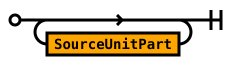
\includegraphics{grammar/sourceunit.jpg}
\caption{SourceUnit}
\end{figure}

\begin{lstlisting}
rule SourceUnit ::=
    SourceUnitPart *  
  ;
\end{lstlisting}

The SourceUnit rule represents the top-level structure of a smart contract source file. It consists of a sequence of source unit parts.

\subsubsection*{Rule SourceUnitPart}

\begin{figure}[!ht]
\centering
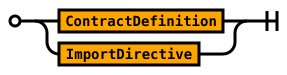
\includegraphics{grammar/sourceunitpart.jpg}
\caption{SourceUnitPart}
\end{figure}

\begin{lstlisting}
rule SourceUnitPart ::=
    ContractDefinition 
  | ImportDirective 
  ;
\end{lstlisting}

The SourceUnitPart rule describes the elements that can appear at the top level of a source file. These elements can be either contract definitions or import directives.

\subsubsection*{Rule ImportDirective}

\begin{figure}[!ht]
\centering
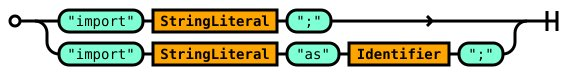
\includegraphics[width=0.8\textwidth]{grammar/importdirective.jpg}
\caption{ImportDirective}
\end{figure}

\begin{lstlisting}
rule ImportDirective ::=
     'import' StringLiteral  ';' 
  |  'import' StringLiteral  'as' Identifier  ';' 
  ;
\end{lstlisting}

The ImportDirective rule defines the syntax for importing other source files into the current file. There are two forms of import directives: a simple import and an import with an alias.

\subsubsection*{Rule Type}

\begin{figure}[!ht]
\centering
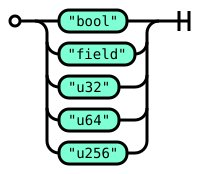
\includegraphics{grammar/type.jpg}
\caption{Type}
\end{figure}

\begin{lstlisting}
rule Type ::=
     'bool' 
  |  'u32' 
  |  'u64' 
  |  'u256' 
  ;
\end{lstlisting}

The Type rule defines the basic types available in the language. These include boolean values (bool),  32-bit unsigned integers (u32), 64-bit unsigned integers (u64), and 256-bit unsigned integers (u256).

\subsubsection*{Rule IdentifierOrError}

\begin{figure}[!ht]
\centering

\includegraphics{grammar/identifierorerror.jpg}
\caption{IdentifierOrError}
\end{figure}

\begin{lstlisting}
rule IdentifierOrError ::=
    Identifier 
  | 
  ;
\end{lstlisting}

The IdentifierOrError rule represents either an identifier or an empty element, which can be useful for optional parts of the grammar.

\subsubsection*{Rule VariableDeclaration}

\begin{figure}[!ht]
\centering
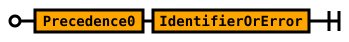
\includegraphics{grammar/variabledeclaration.jpg}
\caption{VariableDeclaration}
\end{figure}

\begin{lstlisting}
rule VariableDeclaration ::=
    Precedence0 IdentifierOrError 
  ;
\end{lstlisting}

The VariableDeclaration rule defines the syntax for declaring a variable. A variable is declared by specifying a type, followed by an optional identifier.

\subsubsection*{Rule StructDefinition}

\begin{figure}[!ht]
\centering
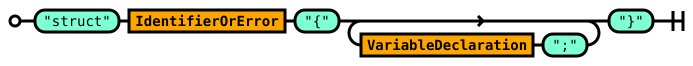
\includegraphics[width=0.8\textwidth]{grammar/structdefinition.jpg}
\caption{StructDefinition}
\end{figure}

\begin{lstlisting}
rule StructDefinition ::=
     'struct' IdentifierOrError  '{' ( VariableDeclaration  ';' ) *   '}' 
  ;
\end{lstlisting}

The StructDefinition rule defines the syntax for declaring a struct type. A struct is a composite data type that groups together variables under a single name.

\subsubsection*{Rule ContractPart}

\begin{figure}[!ht]
\centering
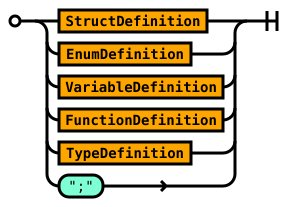
\includegraphics{grammar/contractpart.jpg}
\caption{ContractPart}
\end{figure}

\begin{lstlisting}
rule ContractPart ::=
    StructDefinition 
  | EnumDefinition 
  | VariableDefinition 
  | FunctionDefinition 
  | TypeDefinition 
  |  ';' 
  ;
\end{lstlisting}

The ContractPart rule defines the elements that can appear within a contract definition. These elements include struct definitions, enum definitions, variable definitions, function definitions, and type definitions.

\subsubsection*{Rule ContractDefinition}

\begin{figure}[!ht]
\centering
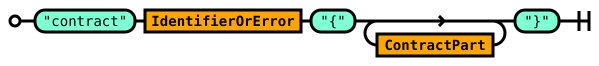
\includegraphics[width=0.8\textwidth]{grammar/contractdefinition.jpg}
\caption{ContractDefinition}
\end{figure}

\begin{lstlisting}
rule ContractDefinition ::=
     'contract' IdentifierOrError  '{' ( ContractPart ) *   '}' 
  ;
\end{lstlisting}

The ContractDefinition rule defines the syntax for declaring a smart contract. A contract is a collection of data and functions that can be executed on a blockchain.

\subsubsection*{Rule EnumDefinition}

\begin{figure}[!ht]
\centering
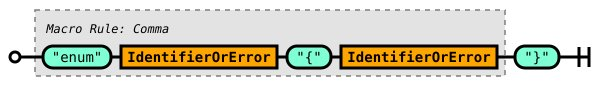
\includegraphics[width=0.8\textwidth]{grammar/enumdefinition.jpg}
\caption{EnumDefinition}
\end{figure}

\begin{lstlisting}
rule EnumDefinition ::=
     'enum' IdentifierOrError  '{' Comma!(IdentifierOrError)  '}' 
  ;
\end{lstlisting}

The EnumDefinition rule defines the syntax for declaring an enumeration type. An enumeration is a data type consisting of a set of named values.

\subsubsection*{Rule VariableDefinition}

\begin{figure}[!ht]
\centering
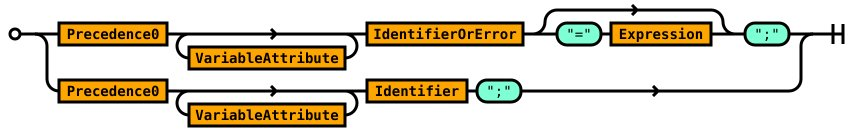
\includegraphics[width=0.8\textwidth]{grammar/variabledefinition.jpg}
\caption{VariableDefinition}
\end{figure}

\begin{lstlisting}
rule VariableDefinition ::=
    Precedence0 VariableAttribute *  IdentifierOrError (  '=' Expression ) ?   ';' 
  | Precedence0 VariableAttribute *  Identifier  ';' 
  ;
\end{lstlisting}

The VariableDefinition rule defines the syntax for defining a variable within a contract. Variables can have attributes such as "const" or "mut" to indicate whether they are constant or mutable.

\subsubsection*{Rule TypeDefinition}

\begin{figure}[!ht]
\centering
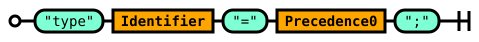
\includegraphics[width=0.8\textwidth]{grammar/typedefinition.jpg}
\caption{TypeDefinition}
\end{figure}

\begin{lstlisting}
rule TypeDefinition ::=
     'type' Identifier  '=' Precedence0  ';' 
  ;
\end{lstlisting}

The TypeDefinition rule defines the syntax for creating a new type alias. A type alias is a way to give a new name to an existing type, which can be useful for improving code readability and maintainability.

\subsubsection*{Rule VariableAttribute}

\begin{figure}[!ht]
\centering
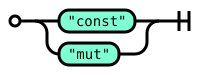
\includegraphics{grammar/variableattribute.jpg}
\caption{VariableAttribute}
\end{figure}

\begin{lstlisting}
rule VariableAttribute ::=
'const'
| 'mut'
;
\end{lstlisting}

The VariableAttribute rule defines the attributes that can be applied to a variable. There are two possible attributes: \verb|const| and \verb|mut|. The \verb|const| attribute indicates that the variable's value cannot be changed after it is initialized, while the \verb|mut| attribute indicates that the variable's value can be modified.

\subsubsection*{Rule Expression}

\begin{figure}[!ht]
\centering
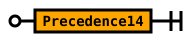
\includegraphics{grammar/expression.jpg}
\caption{Expression}
\end{figure}

\begin{lstlisting}
rule Expression ::=
Precedence14
;
\end{lstlisting}

The Expression rule represents any valid expression in the language. In this case, it refers to the highest level of precedence, Precedence14.

\subsubsection*{Rule Precedence14}

\begin{figure}[!ht]
\centering
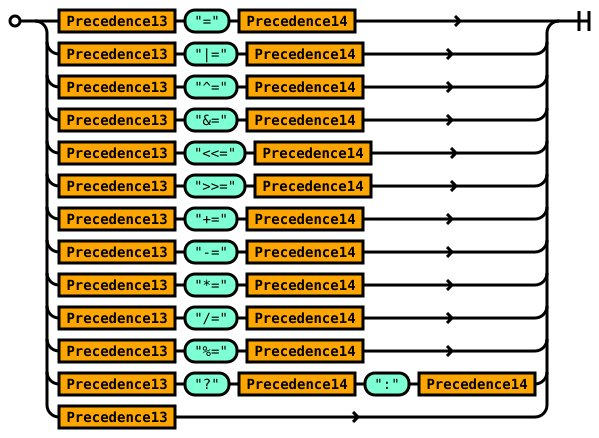
\includegraphics[width=0.8\textwidth]{grammar/precedence14.jpg}
\caption{Precedence14}
\end{figure}

\begin{lstlisting}
rule Precedence14 ::=
Precedence13 '=' Precedence14
| Precedence13 '|=' Precedence14
| Precedence13 '^=' Precedence14
| Precedence13 '&=' Precedence14
| Precedence13 '<<=' Precedence14
| Precedence13 '>>=' Precedence14
| Precedence13 '+=' Precedence14
| Precedence13 '-=' Precedence14
| Precedence13 '*=' Precedence14
| Precedence13 '/=' Precedence14
| Precedence13 '%=' Precedence14
| Precedence13 '?' Precedence14 ':' Precedence14
| Precedence13
;
\end{lstlisting}

The Precedence14 rule defines the various assignment and conditional operators with the highest precedence level. This includes assignment, bitwise OR assignment, bitwise XOR assignment, bitwise AND assignment, left shift assignment, right shift assignment, addition assignment, subtraction assignment, multiplication assignment, division assignment, modulo assignment, and the ternary conditional operator.

\subsubsection*{Rule Precedence13}

\begin{figure}[!ht]
\centering
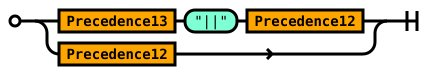
\includegraphics{grammar/precedence13.jpg}
\caption{Precedence13}
\end{figure}

\begin{lstlisting}
rule Precedence13 ::=
Precedence13 '||' Precedence12
| Precedence12
;
\end{lstlisting}

The Precedence13 rule represents the logical OR operator, which has lower precedence than assignment and conditional operators. It allows combining multiple conditions using the ``\verb!||!'' symbol.

\subsubsection*{Rule Precedence12}

\begin{figure}[!ht]
\centering
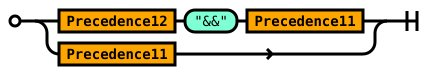
\includegraphics{grammar/precedence12.jpg}
\caption{Precedence12}
\end{figure}

\begin{lstlisting}
rule Precedence12 ::=
Precedence12 '&&' Precedence11
| Precedence11
;
\end{lstlisting}

The Precedence12 rule defines the logical AND operator, which has a lower precedence than the logical OR operator. It is used to combine multiple conditions using the ``\verb|&&|'' symbol.

\subsubsection*{Rule Precedence11}

\begin{figure}[!ht]
\centering
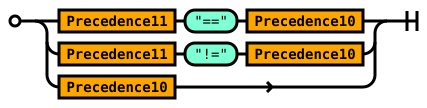
\includegraphics{grammar/precedence11.jpg}
\caption{Precedence11}
\end{figure}

\begin{lstlisting}
rule Precedence11 ::=
    Precedence11  '==' Precedence10 
  | Precedence11  '!=' Precedence10 
  | Precedence10 
  ;
\end{lstlisting}

The Precedence11 rule defines a non-terminal that represents operators with the same precedence level. It has two productions: the first production specifies the equality operator (`\verb|==|') and the next higher precedence non-terminal Precedence10, while the second production specifies the inequality operator (`\verb|!=|') and Precedence10. If neither of these cases applies, Precedence10 is directly considered as the result of this rule. This rule is a useful part of writing a parser or compiler for a programming language, as it can be used to specify operator precedence and associativity.

\subsubsection*{Rule Precedence10}

\begin{figure}[!ht]
\centering
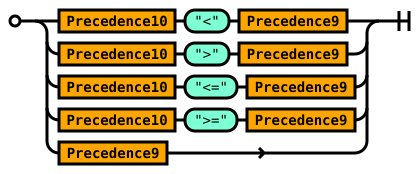
\includegraphics{grammar/precedence10.jpg}
\caption{Precedence10}
\end{figure}

\begin{lstlisting}
rule Precedence10 ::=
    Precedence10  '<' Precedence9 
  | Precedence10  '>' Precedence9 
  | Precedence10  '<=' Precedence9 
  | Precedence10  '>=' Precedence9 
  | Precedence9 
  ;
\end{lstlisting}

The Precedence10 rule defines a non-terminal that represents operators with the same precedence level. It has five productions, each representing a comparison operator (`\verb|<|', `\verb|>|', `\verb|<=|', `\verb|>=|'), followed by the next higher precedence non-terminal Precedence9. If none of these cases apply, Precedence9 is directly considered as the result of this rule. This rule is often used in writing a parser or compiler for a programming language, as it specifies the precedence and associativity of comparison operators.

\subsubsection*{Rule Precedence9}

\begin{figure}[!ht]
\centering
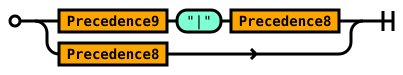
\includegraphics{grammar/precedence9.jpg}
\caption{Precedence9}
\end{figure}

\begin{lstlisting}
rule Precedence9 ::=
    Precedence9  '|' Precedence8 
  | Precedence8 
  ;
\end{lstlisting}

The Precedence9 rule defines a non-terminal that represents operators with the same precedence level. It has two productions: the first production specifies the logical OR operator (`\verb!|!') and the next higher precedence non-terminal Precedence8, while the second production simply specifies Precedence8. If neither of these cases applies, Precedence8 is directly considered as the result of this rule. This rule is often used in writing a parser or compiler for a programming language, as it specifies the precedence and associativity of logical OR operators.

\subsubsection*{Rule Precedence8}

\begin{figure}[!ht]
\centering
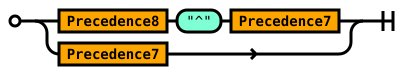
\includegraphics{grammar/precedence8.jpg}
\caption{Precedence8}
\end{figure}

\begin{lstlisting}
rule Precedence8 ::=
    Precedence8  '^' Precedence7 
  | Precedence7 
  ;
\end{lstlisting}

The Precedence8 rule defines a non-terminal that represents operators with the same precedence level. It has two productions: the first production specifies the bitwise XOR operator (`\verb|^|') and the next higher precedence non-terminal Precedence7, while the second production simply specifies Precedence7. If neither of these cases applies, Precedence7 is directly considered as the result of this rule. This rule is often used in writing a parser or compiler for a programming language, as it specifies the precedence and associativity of bitwise XOR operators.

\subsubsection*{Rule Precedence7}

\begin{figure}[!ht]
\centering
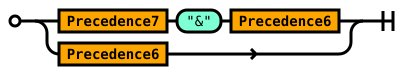
\includegraphics{grammar/precedence7.jpg}
\caption{Precedence7}
\end{figure}

\begin{lstlisting}
rule Precedence7 ::=
    Precedence7  '&' Precedence6 
  | Precedence6 
  ;
\end{lstlisting}

The Precedence7 rule defines a non-terminal that represents operators with the same precedence level. It has two productions: the first production specifies the bitwise AND operator (`\verb|&|') and the next higher precedence non-terminal Precedence6, while the second production simply specifies Precedence6. If neither of these cases applies, Precedence6 is directly considered as the result of this rule. This rule is often used in writing a parser or compiler for a programming language, as it specifies the precedence and associativity of bitwise AND operators.

\subsubsection*{Rule Precedence6}

\begin{figure}[!ht]
\centering
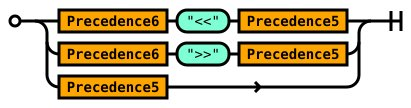
\includegraphics{grammar/precedence6.jpg}
\caption{Precedence6}
\end{figure}

\begin{lstlisting}
rule Precedence6 ::=
    Precedence6  '<<' Precedence5 
  | Precedence6  '>>' Precedence5 
  | Precedence5 
  ;
\end{lstlisting}

The Precedence6 rule defines a non-terminal that represents operators with the same precedence level. It has three productions: the first production specifies the bitwise left shift operator (`\verb|<<|') and the next higher precedence non-terminal Precedence5, the second production specifies the bitwise right shift operator (`\verb|>>|') and Precedence5, while the third production simply specifies Precedence5. If neither of the first two cases applies, Precedence5 is directly considered as the result of this rule. This rule is often used in writing a parser or compiler for a programming language, as it specifies the precedence and associativity of bitwise left shift and bitwise right shift operators.

\subsubsection*{Rule Precedence5}

\begin{figure}[!ht]
\centering
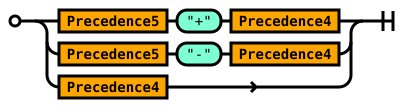
\includegraphics{grammar/precedence5.jpg}
\caption{Precedence5}
\end{figure}

\begin{lstlisting}
rule Precedence5 ::=
    Precedence5  '+' Precedence4 
  | Precedence5  '-' Precedence4 
  | Precedence4 
  ;
\end{lstlisting}

The Precedence5 rule defines a non-terminal that represents operators with the same precedence level. It has three productions: the first production specifies the addition operator (`\verb|+|') and the next higher precedence non-terminal Precedence4, the second production specifies the subtraction operator (`\verb|-|') and Precedence4, while the third production simply specifies Precedence4. If neither of the first two cases applies, Precedence4 is directly considered as the result of this rule. This rule is often used in writing a parser or compiler for a programming language, as it specifies the precedence and associativity of addition and subtraction operators.

\subsubsection*{Rule Precedence4}

\begin{figure}[!ht]
\centering
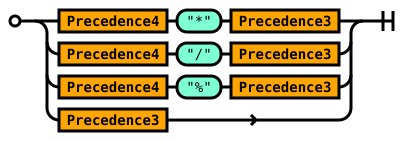
\includegraphics{grammar/precedence4.jpg}
\caption{Precedence4}
\end{figure}

\begin{lstlisting}
rule Precedence4 ::=
    Precedence4  '*' Precedence3 
  | Precedence4  '/' Precedence3 
  | Precedence4  '%' Precedence3 
  | Precedence3 
  ;
\end{lstlisting}

The Precedence4 rule defines a non-terminal that represents operators with the same precedence level. It has four productions: the first production specifies the multiplication operator (`\verb|*|') and the next higher precedence non-terminal Precedence3, the second production specifies the division operator (`'\verb|/|') and Precedence3, the third production specifies the modulus (or remainder) operator (`\verb|%|') and Precedence3, while the fourth production simply specifies Precedence3. If none of the first three cases apply, Precedence3 is directly considered as the result of this rule. This rule is often used in writing a parser or compiler for a programming language, as it specifies the precedence and associativity of multiplication, division, and modulus operators.

\subsubsection*{Rule Precedence3}

\begin{figure}[!ht]
\centering
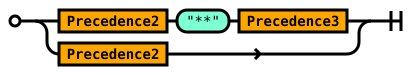
\includegraphics{grammar/precedence3.jpg}
\caption{Precedence3}
\end{figure}

\begin{lstlisting}
rule Precedence3 ::=
    Precedence2  '**' Precedence3 
  | Precedence2 
  ;
\end{lstlisting}



The Precedence3 rule defines a non-terminal that represents operators with the same precedence level. It has two productions: the first production specifies the exponentiation operator (`\verb|**|') and the next higher precedence non-terminal Precedence2, while the second production simply specifies Precedence2. If the first case applies, Precedence3 is considered as the result of the operation Precedence2 raised to the power of Precedence3. Otherwise, Precedence2 is directly considered as the result of this rule. This rule is often used in writing a parser or compiler for a programming language, as it specifies the precedence and associativity of exponentiation operators.

\subsubsection*{Rule Precedence2}

\begin{figure}[!ht]
\centering
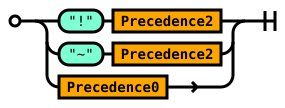
\includegraphics{grammar/precedence2.jpg}
\caption{Precedence2}
\end{figure}

\begin{lstlisting}
rule Precedence2 ::=
     '!' Precedence2 
  |  '~' Precedence2 
  | Precedence0 
  ;
\end{lstlisting}

The Precedence2 rule defines a non-terminal that represents operators with the same precedence level. It has three productions: the first production specifies the logical NOT operator (`\verb|!|') and the same precedence non-terminal Precedence2, the second production specifies the bitwise NOT operator (`\verb|~|') and Precedence2, while the third production simply specifies Precedence0. If either of the first two cases applies, the operator is applied to the result of Precedence2. Otherwise, Precedence0 is directly considered as the result of this rule. This rule is often used in writing a parser or compiler for a programming language, as it specifies the precedence and associativity of logical NOT and bitwise NOT operators.
\subsubsection*{Rule NamedArgument}

\begin{figure}[!ht]
\centering
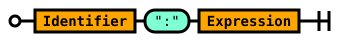
\includegraphics{grammar/namedargument.jpg}
\caption{NamedArgument}
\end{figure}

\begin{lstlisting}
rule NamedArgument ::=
    Identifier  ':' Expression 
  ;
\end{lstlisting}

The NamedArgument rule defines a non-terminal that represents a named argument in a function or method call. It consists of an Identifier followed by a colon and an Expression. The Identifier represents the name of the argument, while the Expression represents its value. This rule is often used in programming languages that support named arguments, allowing for more readable and self-documenting code.

\subsubsection*{Rule FunctionCall}

\begin{figure}[!ht]
\centering
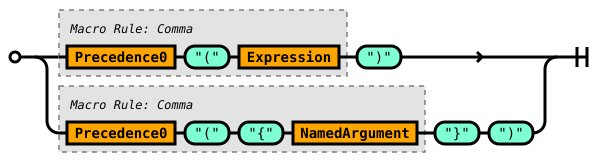
\includegraphics[width=0.8\textwidth]{grammar/functioncall.jpg}
\caption{FunctionCall}
\end{figure}

\begin{lstlisting}
rule FunctionCall ::=
    Precedence0  '(' Comma!(Expression)  ')' 
  | Precedence0  '('  '{' Comma!(NamedArgument)  '}'  ')' 
  ;
\end{lstlisting}

The FunctionCall rule defines a non-terminal that represents a function or method call. It has two productions: the first production specifies an ordered argument list, where the function or method is represented by Precedence0, and the arguments are represented by a comma-separated list of Expression. The second production specifies a named argument list, where the function or method is represented by Precedence0, and the arguments are represented by a comma-separated list of NamedArgument enclosed in braces. This rule is often used in programming languages to represent function or method calls, with the syntax varying depending on the language's support for named arguments and other features.

\subsubsection*{Rule Precedence0}

\begin{figure}[!ht]
\centering
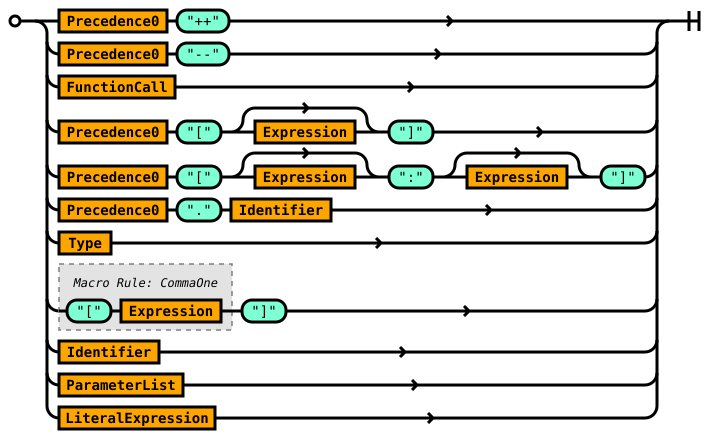
\includegraphics[width=0.8\textwidth]{grammar/precedence0.jpg}
\caption{Precedence0}
\end{figure}

\begin{lstlisting}
rule Precedence0 ::=
    Precedence0  '++' 
  | Precedence0  '--' 
  | FunctionCall 
  | Precedence0  '[' Expression ?   ']' 
  | Precedence0  '[' Expression ?   ':' Expression ?   ']' 
  | Precedence0  '.' Identifier 
  | Type 
  |  '[' CommaOne!(Expression)  ']' 
  | Identifier 
  | ParameterList 
  | LiteralExpression 
  ;
\end{lstlisting}

The Precedence0 rule defines a non-terminal that represents primary expressions, which are the building blocks of more complex expressions. It has multiple productions, including the increment and decrement operators (`\verb|++|' and `\verb|--|'), function or method calls (represented by the non-terminal FunctionCall), array indexing with an Expression inside square brackets, slice notation with two optional Expression separated by a colon inside square brackets, accessing a member of an object using a dot and an Identifier, type names (represented by the non-terminal Type), an array literal with one or more comma-separated Expression enclosed in square brackets, an Identifier, a ParameterList, and a LiteralExpression. These productions specify the most basic elements that can be combined to form more complex expressions in a programming language.

\subsubsection*{Rule LiteralExpression}

\begin{figure}[!ht]
\centering
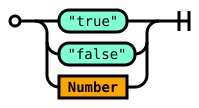
\includegraphics{grammar/literalexpression.jpg}
\caption{LiteralExpression}
\end{figure}

\begin{lstlisting}
rule LiteralExpression ::=
     'true' 
  |  'false' 
  | Number 
  ;
\end{lstlisting}

The LiteralExpression rule defines a non-terminal that represents literal values in a programming language. It has three productions: the first production specifies the Boolean value true, the second production specifies the Boolean value false, and the third production specifies a numeric literal value represented by the non-terminal Number. This rule is often used in programming languages to represent literal values that can be used in expressions, such as Boolean values and numeric constants.

\subsubsection*{Rule Parameter}

\begin{figure}[!ht]
\centering
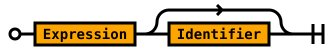
\includegraphics{grammar/parameter.jpg}
\caption{Parameter}
\end{figure}

\begin{lstlisting}
rule Parameter ::=
    Expression Identifier ?  
  ;
\end{lstlisting}

The Parameter rule defines a non-terminal that represents a parameter in a function or method declaration. It consists of an Expression followed by an optional Identifier. The Expression represents the default value of the parameter, while the Identifier represents its name. If the Identifier is not specified, the parameter is treated as an anonymous parameter. This rule is often used in programming languages to define the parameters of functions or methods, allowing the caller to pass arguments to the function or method at runtime.

\subsubsection*{Rule OptParameter}

\begin{figure}[!ht]
\centering

\includegraphics{grammar/optparameter.jpg}
\caption{OptParameter}
\end{figure}

\begin{lstlisting}
rule OptParameter ::=
    Parameter ?  
  ;
\end{lstlisting}

The OptParameter rule defines a non-terminal that represents an optional parameter in a function or method declaration. It consists of an optional Parameter. If the Parameter is present, it specifies a parameter with a default value and an optional name, while if it is absent, there is no default value and no name. This rule is often used in programming languages to provide optional parameters to functions or methods, allowing the caller to omit them if they are not needed.

\subsubsection*{Rule ParameterList}

\begin{figure}[!ht]
\centering
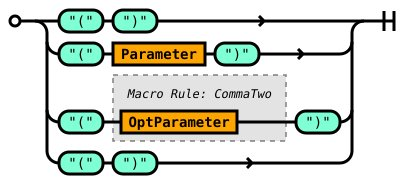
\includegraphics{grammar/parameterlist.jpg}
\caption{ParameterList}
\end{figure}

\begin{lstlisting}
rule ParameterList ::=
     '('  ')' 
  |  '(' Parameter  ')' 
  |  '(' CommaTwo!(OptParameter)  ')' 
  |  '('  ')' 
  ;
\end{lstlisting}

The ParameterList rule defines a non-terminal that represents a list of parameters in a function or method declaration. It has four productions: the first production specifies an empty parameter list, the second production specifies a single parameter, the third production specifies two or more parameters separated by commas, and the fourth production again specifies an empty parameter list. Each parameter is represented by the OptParameter non-terminal, which itself represents an optional parameter with an optional name and default value. This rule is often used in programming languages to define the parameters of functions or methods, allowing the caller to pass arguments to the function or method at runtime.

\subsubsection*{Rule BlockStatementOrSemiColon}

\begin{figure}[!ht]
\centering
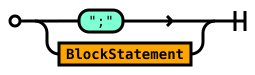
\includegraphics{grammar/blockstatementorsemicolon.jpg}
\caption{BlockStatementOrSemiColon}
\end{figure}

\begin{lstlisting}
rule BlockStatementOrSemiColon ::=
     ';' 
  | BlockStatement 
  ;
\end{lstlisting}

The BlockStatementOrSemiColon rule defines a non-terminal that represents either a semicolon or a block statement in a programming language. It has two productions: the first production specifies a semicolon, and the second production specifies a BlockStatement, which can contain one or more statements enclosed in curly braces. This rule is often used in programming languages to represent the end of a statement or the beginning of a block of statements. If the BlockStatementOrSemiColon is a semicolon, it is typically used to indicate the end of a single statement. If it is a block statement, it is typically used to group multiple statements into a single block that can be executed together.

\subsubsection*{Rule FunctionDefinition}

\begin{figure}[!ht]
\centering
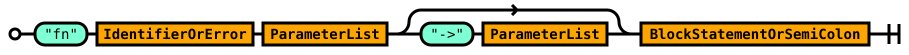
\includegraphics[width=0.8\textwidth]{grammar/functiondefinition.jpg}
\caption{FunctionDefinition}
\end{figure}


\begin{lstlisting}
rule FunctionDefinition ::=
     'fn' IdentifierOrError ParameterList (  '->' ParameterList ) ?  BlockStatementOrSemiColon 
  ;
\end{lstlisting}

The FunctionDefinition rule defines a non-terminal that represents a function definition in a programming language. It consists of the keyword 'fn', followed by an identifier that represents the name of the function, followed by a ParameterList that represents the parameters of the function, and an optional ParameterList that represents the return type of the function. Finally, it ends with a BlockStatementOrSemiColon that represents the body of the function. This rule is often used in programming languages to define functions, which are reusable blocks of code that can be called from other parts of the program. The parameters of the function represent the input values that the function accepts, while the return type represents the output value that the function returns.

\subsubsection*{Rule BlockStatement}

\begin{figure}[!ht]
\centering
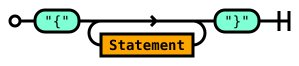
\includegraphics{grammar/blockstatement.jpg}
\caption{BlockStatement}
\end{figure}

\begin{lstlisting}
rule BlockStatement ::=
     '{' Statement *   '}' 
  ;
\end{lstlisting}

The BlockStatement rule defines a non-terminal that represents a block of statements in a programming language. It consists of an opening curly brace, followed by zero or more statements, and finally, a closing curly brace. The statements can be any valid statement in the programming language. This rule is often used in programming languages to group multiple statements together into a single block that can be executed as a unit. A block statement can be used in a variety of contexts, such as in a function body, a loop body, or an if statement body. The block statement allows the programmer to treat multiple statements as a single entity and can be used to make the code more organized and easier to read.

\subsubsection*{Rule OpenStatement}

\begin{figure}
\centering
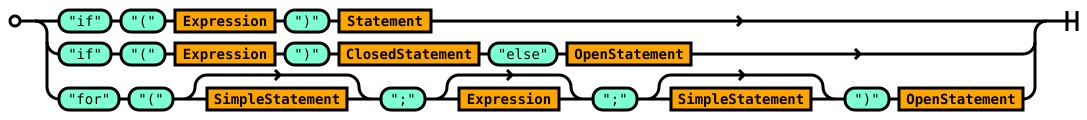
\includegraphics[width=0.8\textwidth]{grammar/openstatement.jpg}
\caption{OpenStatement}
\end{figure}

\begin{lstlisting}
rule OpenStatement ::=
     'if'  '(' Expression  ')' Statement 
  |  'if'  '(' Expression  ')' ClosedStatement  'else' OpenStatement 
  |  'for'  '(' SimpleStatement ?   ';' Expression ?   ';' SimpleStatement ?   ')' OpenStatement 
  ;
\end{lstlisting}

The OpenStatement rule defines a non-terminal that represents an open statement in a programming language. It has three productions: the first production specifies an ``if'' statement with a single statement in its body; the second production specifies an ``if-else'' statement with two sub-statements, one for the ``if'' condition and one for the ``else'' condition; the third production specifies a ``for'' loop with an optional initialization statement, an optional condition, and an optional post-statement, followed by an open statement body. This rule is often used in programming languages to control the flow of execution based on certain conditions or to perform iterative operations on a set of data. The ``if'' statement is used to execute a block of code if a certain condition is true. The ``if-else'' statement is used to execute one of two blocks of code based on whether a certain condition is true or false. The ``for'' loop is used to execute a block of code multiple times while a certain condition is true, and it includes an optional initialization statement, an optional condition, and an optional post-statement.

\subsubsection*{Rule ClosedStatement}

\begin{figure}
\centering
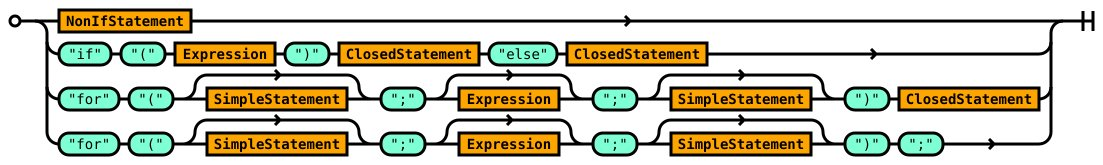
\includegraphics[width=0.8\textwidth]{grammar/closedstatement.jpg}
\caption{ClosedStatement}
\end{figure}

\begin{lstlisting}
rule ClosedStatement ::=
    NonIfStatement 
  |  'if'  '(' Expression  ')' ClosedStatement  'else' ClosedStatement 
  |  'for'  '(' SimpleStatement ?   ';' Expression ?   ';' SimpleStatement ?   ')' ClosedStatement 
  |  'for'  '(' SimpleStatement ?   ';' Expression ?   ';' SimpleStatement ?   ')'  ';' 
  ;
\end{lstlisting}

The ClosedStatement rule defines a non-terminal that represents a closed statement in a programming language. It has four productions: the first production specifies a non-``if'' statements, such as a loop or a function call; the second production specifies an ``if-else'' statement with two sub-statements, both of which are closed statements; the third production specifies a ``for'' loop with an optional initialization statement, an optional condition, and an optional post-statement, followed by a closed statement body; the fourth production specifies a ``for'' loop with an optional initialization statement, an optional condition, and an optional post-statement, followed by a semicolon. This rule is often used in programming languages to control the flow of execution based on certain conditions or to perform iterative operations on a set of data. The closed statement differs from the open statement in that it contains a complete sub-statement within its body.

\subsubsection*{Rule Statement}

\begin{figure}
\centering
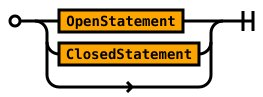
\includegraphics{grammar/statement.jpg}
\caption{Statement}
\end{figure}

\begin{lstlisting}
rule Statement ::=
    OpenStatement 
  | ClosedStatement 
  | 
  ;
\end{lstlisting}

This rule is used to define the structure of statements in a programming language. Statements are used to express an action that needs to be carried out, such as assigning a value to a variable or looping over a set of data. The Statement rule is often used in the context of defining control structures like loops and conditionals.

\subsubsection*{Rule SimpleStatement}

\begin{figure}
  \centering
  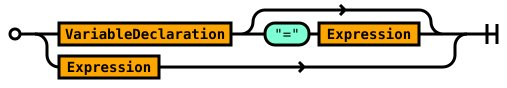
\includegraphics[width=0.8\textwidth]{grammar/simplestatement.jpg}
  \caption{SimpleStatement}
  \end{figure}

\begin{lstlisting}
rule SimpleStatement ::=
    VariableDeclaration (  '=' Expression ) ?  
  | Expression 
  ;
\end{lstlisting}

The SimpleStatement rule is used to define a simple statement in a programming language. It has two possible productions. The first production specifies a VariableDeclaration, which may or may not be followed by an \verb|=| sign and an Expression. This allows for the declaration of a variable with an optional initial value. The second production specifies an Expression, which is a piece of code that evaluates to a value.

\subsubsection*{Rule NonIfStatement}

\begin{figure}
  \centering
  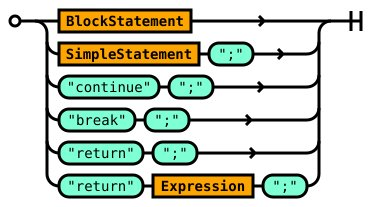
\includegraphics{grammar/nonifstatement.jpg}
  \caption{NonIfStatement}
  \end{figure}

\begin{lstlisting}
rule NonIfStatement ::=
    BlockStatement 
  | SimpleStatement  ';' 
  |  'continue'  ';' 
  |  'break'  ';' 
  |  'return'  ';' 
  |  'return' Expression  ';' 
  ;
\end{lstlisting}

The NonIfStatement rule is used to define a non-conditional statement in a programming language. It has several possible productions, including a BlockStatement and a SimpleStatement followed by a semicolon.

The BlockStatement production allows for a block of code to be executed as a single unit and is often used to group multiple statements. The SimpleStatement followed by a semicolon production allows for a single statement to be executed.

In addition, the rule specifies three special types of statements: continue, break, and return. The continue statement is used to skip to the next iteration of a loop, while the break statement is used to exit a loop. The return statement is used to exit a function and optionally return a value.

Overall, the NonIfStatement rule is an important part of defining the syntax of a programming language and is used to express a wide range of statements and behaviors.

\subsubsection*{Macro Comma}

\begin{figure}
  \centering
  \includegraphics{grammar/comma.jpg}
  \caption{Comma}
  \end{figure}

\begin{lstlisting}
macro Comma<T> ::=
    
  | CommaOne!(T) 
  ;
\end{lstlisting}

This is a macro definition for a comma-separated list of elements of type T. It allows for zero or more elements separated by commas. The \verb|!| symbol after the macro name indicates that the macro is left-recursive, meaning it can be applied repeatedly until it no longer matches. The \verb|CommaOne!| in the definition means that the macro should match at least one element before the optional commas.

\subsubsection*{Macro CommaOne}

\begin{figure}
  \centering
  \includegraphics{grammar/commaone.jpg}
  \caption{CommaOne}
  \end{figure}

\begin{lstlisting}
macro CommaOne<T> ::=
    T (  ',' T ) *  
  ;
\end{lstlisting}

This is a macro definition for a comma-separated list of one or more elements of type \verb|T|. It first matches a single element of type \verb|T|, followed by zero or more occurrences of a comma followed by another element of type \verb|T|. The \verb|*| after the second parentheses indicates that this sequence can repeat zero or more times. This macro enforces that there must be at least one element in the comma-separated list.

\subsubsection*{Macro CommaTwo}

\begin{figure}
  \centering
  \includegraphics{grammar/commatwo.jpg}
  \caption{CommaTwo}
  \end{figure}

\begin{lstlisting}
macro CommaTwo<T> ::=
    T (  ',' T ) +  
  ;
\end{lstlisting}

The CommaTwo macro is used to match one or more occurrences of the same non-terminal symbol separated by commas.

\subsubsection*{Rule Number}

\begin{figure}
  \centering
  \includegraphics{grammar/number.jpg}
  \caption{Number}
  \end{figure}

\begin{lstlisting}
rule Number ::=
     'r#([1-9][0-9]*|0)#' 
  |  'r#0x[0-9A-Fa-f]*#' 
  ;
\end{lstlisting}

The Number rule is used to define a number in a programming language. It has two possible productions. The first production matches a decimal number, while the second production matches a hexadecimal number.

\subsubsection*{Rule Identifier}

\begin{figure}
  \centering
  \includegraphics{grammar/identifier.jpg}
  \caption{Identifier}
  \end{figure}

\begin{lstlisting}
rule Identifier ::=
'r#[$_][a-zA-Z][a-zA-Z$_0-9]#'
;
\end{lstlisting}

The Identifier rule is used to define an identifier in a programming language. It matches a sequence of characters that starts with a letter or underscore, followed by zero or more letters, numbers, underscores, or dollar signs.

\subsubsection*{Rule StringLiteral}

\begin{figure}
  \centering
  \includegraphics{grammar/stringliteral.jpg}
  \caption{StringLiteral}
  \end{figure}

\begin{lstlisting}
rule StringLiteral ::=
'r#\[^\]*\#'
;
\end{lstlisting}

The StringLiteral rule is used to define a string literal in a programming language. It matches a sequence of characters surrounded by square brackets.

\subsection{Smart Contracts}


Ola contracts allow users to write complex business logic that will be deployed to Ola's L2 network, and cross-contract calls can be written between different contracts just like solidity.

\subsubsection{Simple Examples}

The following example shows a recursive and non-recursive Ola smart contract implementation of Fibonacci numbers.

\begin{lstlisting}
contract Fibonacci {

    fn main() {
       fib_non_recursive(10);
    }

    fn fib_recursive(u32 n) -> (u32) {
        if (n == 0 || n == 1) {
            return 1;
        }
        return fib_recursive(n -1) + fib_recursive(n -2);
    }

    fn fib_non_recursive(u32 n) -> (u32) {
        u32 first = 0;
        u32 second = 1;
        u32 third = 1;
        for (u32 i = 2; i <= n; i++) {
             third = first + second;
             first = second;
             second = third;
        }
        return third;
    }

}
\end{lstlisting}

The following shows a simple Person contract that contains a person structure, assigns a value to the Person structure, and reads the status of the person.

\begin{lstlisting}
contract Person {

    enum Sex {
        Man,
        Women
    }

    struct Person {
        Sex s;
        u32 age;
        u256 id;
    }

    Person p;

    fn newPerson(Sex s, u32 age, u256 id) {
        p = Person(s, age, id);
    }

    fn getPersonId() -> (u256) {
        return p.id;
    }

    fn getAge() -> (u32) {
        return p.age;
    }
}
\end{lstlisting}

\subsubsection{Multiple files}

For better project organization and clearer logic, it is common to split the contents of a file into multiple files. Ola language supports the import of another contract within a contract through the `import` keyword.

An example of a multi-file contract is shown below.

\textbf{Contract RectangularCalculator}

\begin{lstlisting}
contract RectangularCalculator {
  
    fn rectangle(u32 w, u32 h) -> (u32 s, u32 p) {
        s = w * h;
        p = 2 * (w + h);
        // Returns a variable with the same name, the return can be ignored
        //return (s, p)
    }
}
\end{lstlisting}

\textbf{Contract ShapeCalculator}

\begin{lstlisting}
contract SquareCalculator {

    fn square(u32 w) -> (u32 s, u32 p) {
        s = w * w;
        p = 4 * w;
        return (s, p);
    }
}
\end{lstlisting}

\textbf{Contract Calculator}

\begin{lstlisting}
import "./RectangularCalculator";
import "./SquareCalculator";

contract Calculator {
  
    fn sum(u32 w, u32 h) -> (u32 s, u32 p) {
        (u32 rectangle_s, u32  rectangle_p) = rectangle(w, h);
        (u32 square_s, u32 square_p) = square(w);
        return (rectangle_s + square_s, rectangle_p + square_p);
    }
}
\end{lstlisting}


\subsection{Ola Compiler}

\subsubsection{Ola Compiler Introduction}

The Ola-lang compiler compiles the high-level Ola contract code into OlaAsm assembly code supported by OlaVM. 

The general pipeline process is as follows:

\begin{figure}[!htp]
    \centering
    \includegraphics[width=0.6\textwidth]{ola-lang-intro.jpg}
    \caption{Ola-lang pipeline}
    \label{fig:ola-lang-intro}
\end{figure}
program->ir process and structure detailed diagram (expand below)

Structure:

    Tokens

    Ast

    IR

IR process

Devices:

    Lex and Syntax

    Semantics

    IR generation
\subsubsection{Ola Compiler Backend}

Detailed diagram of ir->asm flow and structure (expanded below)

Structure:

    lists

    insts

    mcinsts

ABI:

    Function call specification

    Mapping Relationships to Virtual Memory

Devices:

    IR parsing

    Target code generation

        Function call demotion

        Instruction selection

        Register Allocation

        Slot elimination

        Stack frame handling

        Assembly printing

    \begin{itemize}
        \item IR parsing

    IR is composed of the following structure: module -> function -> value -> types.

    Module structure contains Target (triple and datalayout information), Function, Attribute, GlobalVariable.

    Function structure contains name, type information, Visibility, Attribute and Parameter list basic information, and data, Layout.

    Among them, layout contains the sequential logical relationship between basicBlocks and the instructions within them.

    Data contains the specific Value, Instruction, BasicBlock list instances.

    BasicBlock is identified by BasicBlockId and consists of two parts: name and number. Each BB block usually contains one preds and one sucs.

    Instruction is identified by BasicBlockId+InstructionId and usually consists of Opcode, Operand, dest and the Type of its operation.

    Value contains Instruction, Argument, Constant and InlineAsm types.

    Due to the characteristics of the instruction set of olavm, the type is currently mainly i64 type.

        \item IR parsing process

        process: targetDatalayout/targetTriple -> attributeGroup -> localType -> globalVariable -> function -> metadata.

    The function is mainly divided into two parts: parseArgumentList and parseBody.

        \item IR opt pass

    Pre-analysis analysis pass is mainly DominatorTree, conversion transform pass contains dce, mem2reg, sccp.

        \item back-end codegen modules

    bridging ir structure of module, function, and isa related callconv, register and isa, code generation related lower and optimization related pass.

    TargetISA main contains custom TargetInst, Register(RegisterClass/RegisterInfo), lower and modulepasses, callconv, datalayout information.

    Module in addition to inheritance Ir parsed out Module, the description of its Function and ir differ significantly.

    Data information: BasicBlock in the instructions for Target Instruction, register contains VRegs and RegUnit two categories, and contains a vregtoinsts mapping.
    At the same time, Inst in Layout are referred to TargetInst.
    Note that the memory access operations of parameters, local variables, etc. are described by the structure of slot(ptr+offset).

    The lower module provides the process of downgrading LoweringContext to Instruction, and for function calls it also requires copyargstovregs.

    The pass module contains the regalloc and spiller for analyzing the liveness of the pass and the function pass.

        \item back-end process

    Register and insts description

    Function call demotion

    Instruction selection

    eliminateslot

    proepiinserter

    reg allocation and coalescing
    
    \end{itemize}
\subsubsection{Lib funtions}




    \section{Ola-Compiler: A LLVM IR Based Compiler to Generate RISC Assembly}\label{sec:ola-compiler}

\subsection{Ola Compiler Introduction}

The Ola Compiler compiles the high-level Ola contract code into the assembly code supported by OlaVM. 

The general pipeline process is shown as figure \ref{fig:ola-lang-intro}:

\begin{figure}[!htp]
    \centering
    \includegraphics[width=0.8\textwidth]{ola-lang-intro.png}
    \caption{Ola-lang Language and Compiler Pipeline}
    \label{fig:ola-lang-intro}
\end{figure}

As can be seen from the above figure, the frontend of the compiler takes the high-level contract program as input and then compiles it into LLVM Intermediate Representation (IR);
and the backend of the compiler takes the LLVM IR generated by the frontend as input and then compiles it into Ola assembly code.

The assembly code is eventually assembled, linked, loaded, and executed by OlaVM through the toolchain pipeline to generate a trace.

To illustrate the compiler pipeline, the following is an example of a typical u32 type sqrt operation with instructions and Prophet two different versions to show the code generation process.

An example Ola-lang high-level language program for computing sqrt of type u32 with Prophet version is as follows:
\begin{lstlisting}[language=rust]
contract SqrtContract {

    fn main() {
       sqrt_test(4);
    }

    fn sqrt_test(u32 n) -> (u32) {
        u32 b = u32_sqrt(n);
        return b;
    }

}
\end{lstlisting}


An example ola-lang high-level language program for computing sqrt of type u32 with instructions version is as follows:
\begin{lstlisting}[language=rust]
contract SqrtContract {

    fn main() {
       sqrt_test(4);
    }

    fn sqrt_test(u32 a) -> (u32) {
        u32 result = 0;
        if (a > 3) {
            result = a;
            u32 x = a / 2 + 1;
            // assume the maximum iteration is 100
            for (u32 i = 0; i < 100; i++) {
                if (x >= result) break;
                result = x;
                x = (a / x + x) / 2;
            }
        } else if (a != 0) {
            result = 1;
        }
        return result;
    }

}
\end{lstlisting}

\subsection{Ola Language Compiler Front-end}

This section introduces the key components and functionalities of the Ola language compiler front-end. We will discuss the process of lexical analysis, syntax parsing, Abstract Syntax Tree (AST) generation, semantic analysis, and LLVM Intermediate Representation (IR) generation in detail.

The processing flow of the compiler front-end is shown in the following diagram \ref{fig:ola-lang-compiler-frontend}:

\begin{figure}[!ht]
    \centering
    \includegraphics[width=0.8\textwidth]{ola-lang-compiler-frontend.jpg}
    \caption{Ola-lang Compiler Frontend}
    \label{fig:ola-lang-compiler-frontend}
\end{figure}



\subsubsection{Ola Language Parser}
\subsubsection*{Lexical Analysis}
Lexical analysis is the first stage of the compiler front-end. In this phase, the goal is to break down the source code into a series of tokens. The Ola language lexer will handle the following elements:
\begin{itemize}
\item Keywords
\item Identifiers
\item Operators
\item Literals (such as strings, numbers, and boolean values)
\item Comments
\item Delimiters (such as parentheses and commas)
\end{itemize}
Additionally, the lexer will eliminate whitespace and comments, ensuring a clean token stream for the next stage.

\subsubsection*{Syntax Parsing}
Syntax parsing is the process of transforming the tokens generated in the lexical analysis phase into an Abstract Syntax Tree (AST). The Ola language compiler will implement a top-down parser, such as a Recursive Descent Parser, to support Ola language's grammar.

This section will also discuss the implementation of error handling and recovery mechanisms, ensuring that the parser can handle syntax errors gracefully and provide helpful error messages to the user.

\subsubsection*{Abstract Syntax Tree (AST) Generation}
During the syntax parsing phase, the parser will generate an AST representing the program's structure. This section will explain the design of the AST data structures and the process of constructing the AST during parsing. Additionally, it will cover the benefits of using an AST, such as enabling easier manipulation and analysis of the code's structure.

The Ola compiler seamlessly integrates the Lexical Analysis, Syntax Parsing, and Abstract Syntax Tree (AST) Generation processes, forming a cohesive and efficient pipeline. By leveraging the LALRPOP framework, these stages work in harmony, transforming the Ola source code into an AST representation that is suitable for subsequent compiler phases. This unified approach not only simplifies the implementation but also enhances the performance and robustness of the Ola compiler.

By following these steps, the compiler can efficiently convert the Ola source code text into a sequence of tokens:

\begin{itemize}

  \item The first step in implementing the lexical analysis phase of the Ola compiler is to define lexer rules for various token categories, including keywords, identifiers, literals, and operators. These rules should be based on the provided EBNF grammar rules. We created a file named Ola.lalrpop that describes Ola's EBNF grammar rules.

  \item After defining the lexer rules, the next step is to integrate the lexer with the parser. This can be achieved by using the \texttt{lexer} attribute in LALRPOP grammar rules. The \texttt{lexer} attribute specifies which lexer rule should be used to recognize a particular grammar production.

  \item Ola compiler provides error handling and reporting. If the lexer encounters an unexpected character or a malformed token, it generates an error with the corresponding position in the input text. This information can be used to provide helpful error messages to the user.

\end{itemize}

Once the lexical analysis phase is complete, the generated sequence of tokens can be passed to the parser, which will construct an abstract syntax tree (AST) based on the defined grammar rules. This AST can then be further processed by subsequent phases of the Ola compiler, such as semantic analysis, optimization, and code generation, ultimately producing executable code for the target platform.

By leveraging the powerful LALRPOP framework, the Ola compiler can efficiently perform lexical analysis and provide robust error handling, ensuring that the compiler is user-friendly and capable of handling complex Ola source code.

\subsubsection{Semantic Analysis}

The Semantic Analysis phase of the Ola compiler is an extensive process that ensures the program's correctness and consistency. As previously mentioned, this phase consists of several sub-tasks. Here, we delve deeper into each sub-task, providing a more detailed and comprehensive explanation of the process.

\subsubsection*{Symbol Resolution}

The compiler analyzes the program's scope and context to resolve symbols accurately. It distinguishes between local and global variables, function declarations, and type definitions. The symbol table, which holds information about each symbol, is updated as the compiler traverses the AST. During this process, the compiler also checks for naming conflicts and multiple declarations, ensuring that the program adheres to Ola's scoping rules.

\subsubsection*{LibFunction Identification}

In the semantic analysis phase, we will identify all libFunction names that users call. We will also construct prototype code for these LibFunctions and verify whether the parameters used to call them match the parameter types and numbers in the prototype code. If there is a match, we will record them for easy processing of IR generation for Lib Functions in subsequent LLVM IR generation phases.

\subsubsection*{Type Checking}

The compiler ensures that each operation and expression in the program involves operands of compatible types. In this stage, the compiler also infers the types of expressions when necessary and enforces type constraints for function calls, assignments, and arithmetic operations.

\subsubsection*{Control Flow Analysis}

In addition to checking for unreachable code and infinite loops, the control flow analysis process verifies that:

\begin{itemize}
 \item All code paths in a function that should return a value must end with a return statement.
 \item Break and continue statements appear only within loops.
 \item Variables are declared before they are used.
\end{itemize}

\subsubsection*{Constant Expression Evaluation}

During this step, the compiler performs the following tasks:

\begin{itemize}
  \item Evaluates arithmetic and bitwise operations on constant expressions at compile-time, ensuring that the generated code is more efficient.

  \item Detects potential errors, such as array index out-of-bounds, by evaluating expressions that involve constants.

  \item Folds constant expressions, such as mathematical operations or string concatenations, reducing the code size and improving execution efficiency.

\end{itemize}

\subsubsection*{Semantic Validation}
 The final step of the semantic analysis phase consists of several validation checks, including:

\begin{itemize}
  \item Verifying that variables are initialized before they are used.
  \item Ensuring that variables, functions, and types are declared only once within a given scope.
  \item Checking that all required function arguments are provided and that excess arguments are not supplied.
  \item Validating that return statements are used correctly within functions.

\end{itemize}

The Semantic Analysis phase is crucial for the robustness and correctness of the Ola compiler. By performing these comprehensive checks, the compiler can guarantee that the generated code adheres to the language's semantic rules and is free from errors that might lead to unexpected behavior during execution. With a semantically verified AST, the Ola compiler proceeds to the subsequent phases of the compilation process, ensuring the efficient translation of the source code into executable code tailored for the OlaVM.

\subsubsection{Generator: from richAST to LLVM IR}

\subsection{Ola Compiler Backend: from LLVM IR to OlaVM assembly}

Ola compiler backend bridge IR structure of module, function and Instruction Set Architecture(ISA) related callconv, registers and instructions.
Its main features are code generation related lower and optimization related passes.

Target Instruction Set Architecture(ISA) mainly contains custom target instructions, registers which contain register class and register information, call convention and datalayout information.

Module in addition to inheritance IR is parsed out as Module structure, the description of its function and differ significantly with LLVM IR.
Data information of Basic Block(BB) in the instructions target for the instruction, the register contains VRegs(Virtual Registers) and RegUnit(Register Unit) two categories, and contains a VRegs to Instructions(Insts) mapping.
At the same time, instruction in data layout is referred to target instruction. Note that the structure of slot which contains stack base pointer and stack offset describe the memory access operations of parameters, local variables.

The lower provides the process of downgrading IR instruction to target instruction. Specifically it also requires copy parameters to VRegs for function call.

The pass module contains the register allocation(RegAlloc, RA) and spiller for analyzing the liveness of the pass and the function pass.

\subsubsection{Parser: parse LLVM IR to Module insts}

The detailed process is as follows:
    \begin{itemize}
        \item IR parsing

IR is composed of the following structure: module -> function -> value -> types.

(1) Module structure contains Target (triple and datalayout information), Function, Attribute, GlobalVariable.

(2) Function structure contains name, type information, Visibility, Attribute and Parameter list basic information, and data, Layout.

(3) Among them, layout contains the sequential logical relationship between basicBlocks and the instructions within them.

(4) Data contains the specific Value, Instruction, BasicBlock list instances.

(5) BasicBlock is identified by BasicBlockId and consists of two parts: name and number. Each BB block usually contains one preds and one sucs.

(6) Instruction is identified by BasicBlockId+InstructionId and usually consists of Opcode, Operand, dest and the Type of its operation.

(7) Value contains Instruction, Argument, Constant and InlineAsm types.

(8) Due to the characteristics of the instruction set of olavm, the type is currently mainly i64 type.

        \item IR parsing process

process: targetDatalayout/targetTriple -> attributeGroup -> localType -> globalVariable -> function -> metadata.

The function is mainly divided into two parts: parseArgumentList and parseBody.

Its pipeline process is as follow:
\begin{figure}[!htbp]
    \centering
    \includegraphics[width=0.6\textwidth]{ola-lang-backend-parser.jpg}
    \caption{ola-lang backend parser pipeline}
    \label{fig:ola-lang-backend-parser}
\end{figure}
\end{itemize}
\subsubsection{Opt: opt pass on IR insts}

Currently DominatorTree is an mainly analysis pass, conversion transform passes contains dce, mem2reg, sccp.

Its pipeline process is as follows:
\begin{figure}[!htbp]
    \centering
    \includegraphics[width=0.5\textwidth]{ola-lang-backend-ir-opt.jpg}
    \caption{ola-lang backend ir opt}
    \label{fig:ola-lang-backend-ir-opt}
\end{figure}
\subsubsection{ISA description: register and insts}

\begin{itemize}
    \item back-end codegen modules

bridging ir structure of module, function, and isa related callconv, register and isa, code generation related lower, and optimization-related pass.

TargetISA main contains custom TargetInst, Register(RegisterClass/RegisterInfo), lower and modulepasses, callconv, datalayout information.

Module in addition to inheritance Ir parsed out Module, the description of its Function and ir differ significantly.

Data information: BasicBlock in the instructions for Target Instruction, the register contains VRegs and RegUnit two categories, and contains a vregtoinsts mapping.
At the same time, Inst in Layout is referred to TargetInst. Note that the memory access operations of parameters, local variables, etc. are described by the structure of slot(ptr+offset).

The lower module provides the process of downgrading LoweringContext to Instruction, and for function calls it also requires copyargstovregs.

The pass module contains the regalloc and spiller for analyzing the liveness of the pass and the function pass.

        \item back-end process

(1) Register and insts description

The register description is as below:
\begin{table}[!ht]
    \resizebox{\textwidth}{!}{
        \begin{tabular}{|c|c|c|}
            \hline
            \textit{Type}  & \textit{Description} & \textit{Register Group}  \\ \hline
            general registers & general used by program &  $[r0-r8] $ \\ \hline
            return regsiter & return value for return to caller &  $[r0] $ \\ \hline
            parameters rigsters & parameters value for passing arguments &  $ [r1, r2, r3] $ \\ \hline
            tmp registers & tmp alloc for local variables &  $[r4, r5, r6, r7]$ \\ \hline
            stack pointer & function's stack pointer &  $[r8] $ \\ \hline
            special registers & interact with vm: pc for program counter and psp for prophet pointer &   $[pc, psp] $ \\ \hline
        \end{tabular}}
    \caption{Register Description}
    \label{table:register-description}
\end{table}

Insts description is as bellow:

Opcode with register or immediate number:
\begin{lstlisting}[language={}]
    ADDri,
    ADDrr,
    MULri,
    MULrr,

    EQri,
    EQrr,
    ASSERTri,
    ASSERTrr,

    MOVri,
    MOVrr,

    JMPi,
    JMPr,
    CJMPi,
    CJMPr,
    CALL,
    RET,
    END,

    MLOADi,
    MLOADr,
    MSTOREi,
    MSTOREr,

    RANGECHECK,
    AND,
    OR,
    XOR,
    NOT,
    NEQ,
    GTE,

    PROPHET,

    Phi,
\end{lstlisting}

Operand data type:
\begin{lstlisting}[language={}]
    Reg(Reg),
    VReg(VReg),
    Int8(i8),
    Int32(i32),
    Int64(i64),
    MemStart,
    Slot(SlotId),
    Block(BasicBlockId),
    Label(String),
    GlobalAddress(String),
    None,
\end{lstlisting}

\end{itemize}
\subsubsection{ABI Lower: Lowering Function Call}
    
Ola Procedure Call Standard(OPCS) are as follows:

The stack initialization points to the first address of the frame stack after the \texttt{fp} register is loaded.
    
The address will be increased when the \texttt{call} instruction is executed later.
When the \texttt{ret} instruction is executed, the \texttt{fp} register points to the address and falls back.
    
    
the Calling process is as follows:
\begin{itemize}
    \item call label

Caller use \texttt{call} instruction to call a callee as \texttt{call functionLabel}, and \texttt{fp} points to the new frame.\par
The \texttt{pc} address returned by the callee is placed in \texttt{fp-1} which is detected by VM but not visible by the compiler backend.\par
Its instructions pattern are as follows:
\begin{lstlisting}[language={}]
main:
.LBL0_0:
  ...
  call foo
  ...
foo:
.LBL1_0:
  ...
\end{lstlisting}
    \item function address

The address pointed to by \texttt{fp} before the function call is placed in \texttt{fp-2} as \texttt{mstore [r8,-2] r8}.\par
Its instructions pattern are as follows:
\begin{lstlisting}[language={}]
mstore [r8,-2] r8
\end{lstlisting}
    \item passing arguments

Function parameter processing: the first three input parameters are placed in the three registers \texttt{r1}, \texttt{r2}, and \texttt{r3}.
If there are more than 3 parameters, start with the fourth input parameter and descend accordingly in \texttt{fp-3}, \texttt{fp-4}, \texttt{...}. \par
Its instructions pattern are as follows:
\begin{lstlisting}[language={}]
mov r1 vreg1
mload r2 [r8,offset]
mov r3 vreg2
\end{lstlisting}
    \item  local variables

Local variables inside the function start at old \texttt{fp}, and their addresses are stored incrementally.

The single return value is stored in \texttt{r0}. If there are multi return values, it needs to be returned by a memory pointer that return the package data.\par
Instruction pattern for single return value is as follows:
\begin{lstlisting}[language={}]
mov r0 vreg3
\end{lstlisting}
\end{itemize}

The call stack frames layout is as follows \ref{fig:ola-lang-backend-functioncall}:

\begin{figure}[!htp]
    \centering
    \includegraphics[width=0.8\textwidth]{ola-lang-backend-functioncall.jpg}
    \caption{Ola-lang Function Call Stack Frames}
    \label{fig:ola-lang-backend-functioncall}
\end{figure}

For prophet library functions, its instructions pattern as:
\begin{lstlisting}[language={}]
.PROPHET{funcNum}_{prophetNum}:  // bind to prophet label
mov r0 psp  // interact with prophet read-only memory, get return value from prophet pointer
mload r0 [r0,0]  // used returned r0 as indexed addressing
\end{lstlisting}

First \texttt{.PROPHET} label binds to the prophet instance in assembly output.
Then the program interacts with prophet read-only memory, get the return value from prophet pointer \texttt{[psp]} and write the result into \texttt{r0}.
At last, we use \texttt{r0} as indexed addressing to load return values from prophet memory.
\subsubsection{Insts selection: match pattern from ir inst to MCinst}

It match ir insts opcode + operand pattern, then lower the matched pattern to target machine code insts.

Several common patterns such as: 
\begin{table}[!ht]
    \resizebox{\textwidth}{!}{
        \begin{tabular}{|c|c|}
            \hline
            \textit{Pattern Type} & \textit{Description} \\ \hline
            Alloca  & params and vars allocation \\ \hline
            IntBinary & bianary operator \\ \hline
            Load & memory load \\ \hline
            Store & memory store  \\ \hline
            Call & function call \\ \hline
            Return & function call return \\ \hline
            Branch & branch control flow \\ \hline
            Conditional Branch & conditional branch control flow \\ \hline
        \end{tabular}}
    \caption{Instruction Pattern}
    \label{table:Instruction-pattern}
\end{table}

Let's take Conditional Branch for example, it's target insts as follow:
\begin{table}[!ht]
    \resizebox{\textwidth}{!}{
        \begin{tabular}{|c|c|c|c|}
            \hline
            \textit{operator}  & \textit{Reg+Imm} & \textit{Reg+Reg} & \textit{Cycles}  \\ \hline
            == & \makecell{mov tmpReg imm \\ eq tmpReg regA tmpReg \\ cjmp tmpReg labelTrue} & \makecell{eq tmpReg regA regB \\ cjmp tmpReg labelTrue} & \makecell{3inst + 2reg \\ 2inst + 3reg} \\ \hline
            < & \makecell{mov tmpReg1 imm \\ gte tmpReg1 tmpReg1 regA \\ neq tmpReg2 tmpReg1 regA \\and tmpReg2 tmpReg2 tmpReg1 \\ cjmp tmpReg2 labelTrue} & \makecell{gte tmpReg1 regB regA \\ neq tmpReg2 regA regB \\ and tmpReg2 tmpReg1 tmpReg2 \\ cjmp tmpReg2 labelTrue} & \makecell{5inst + 3reg \\ 4inst + 4reg} \\ \hline
            <= & \makecell{mov tmpReg imm \\ gte tmpReg tmpReg regA \\ cjmp tmpReg labelTrue} & \makecell{gte tmpReg regA regB \\ cjmp tmpReg labelTrue} & \makecell{3inst + 2reg \\ 2inst + 3reg} \\ \hline
            > & \makecell{mov tmpReg1 imm \\ gte tmpReg1 regA tmpReg1 \\ neq tmpReg2 tmpReg1 regA \\and tmpReg2 tmpReg2 tmpReg1 \\ cjmp tmpReg2 labelTrue} & \makecell{gte tmpReg1 regA regB \\ neq tmpReg2 regA regB \\ and tmpReg2 tmpReg1 tmpReg2 \\ cjmp tmpReg2 labelTrue} & \makecell{5inst + 3reg \\ 4inst + 4reg} \\ \hline
            >= & \makecell{mov tmpReg imm \\ gte tmpReg regA tmpReg \\ cjmp tmpReg labelTrue} & \makecell{gte tmpReg regA regB \\ cjmp tmpReg labelTrue} & \makecell{3inst + 2reg \\ 2inst + 3reg} \\ \hline
            != & \makecell{mov tmpReg imm \\ neq tmpReg regA tmpReg \\ cjmp tmpReg labelTrue} & \makecell{neq tmpReg regA regB \\ cjmp tmpReg labelTrue} & \makecell{3inst + 2reg \\ 2inst + 3reg} \\ \hline
        \end{tabular}}
    \caption{Conditional Branch Pattern}
    \label{table:conditional-branch-pattern}
\end{table}
\subsubsection{Slot Elimination}

This pass handles the stack slot for local variables.

Its pipeline is as follows:
\begin{lstlisting}[language={}]
VistModule
    | VisitFunction layout
        | VisitBasicBlock
            | Match inst's data operand is Slot type
                | workList: push inst 
    | Computer slot offset
    | foreach workList
        | fixup inst's operand with offset and size
\end{lstlisting}
\subsubsection{Target Instruction Insertion: Prologue and Epilogue}

When the processing is completed after the parameters of the function and the function body, 
as a part of the function it needs to do the corresponding stack space processing at the entrance and exit, respectively.
That is, first calculate the stack size, then the stack is opened at the entrance, and the stack is recycled at the exit.

When there is no function call in the function body, entrance is one add instruction such as:
\begin{lstlisting}[language=rust]
InstructionData {
    opcode: Opcode::ADDri,
    operands: vec![
        Operand::input_output(GR::R8.into()),
        Operand::input_output(GR::R8.into()),
        Operand::input(adj.into()),
    ],
}
\end{lstlisting}

When there is one or multi function call in the function body, entrance is one add inst and one mstore instruction such as:
\begin{lstlisting}[language=rust]
InstructionData {
    opcode: Opcode::ADDri,
    operands: vec![
        Operand::input_output(GR::R8.into()),
        Operand::input_output(GR::R8.into()),
        Operand::input(adj.into()),
    ],
}

InstructionData {
    opcode: Opcode::MSTOREr,
    operands: vec![
        Operand::output(GR::R8.into()),
        Operand::input(GR::R8.into()),
    ],
}
\end{lstlisting}

While the exit is one sub operator which is expressed as add instruction such as:
\begin{lstlisting}[language=rust]
InstructionData {
    opcode: Opcode::ADDri,
    operands: vec![
        Operand::output(GR::R8.into()),
        Operand::input_output(GR::R8.into()),
        Operand::input((-adj).into()),
    ],
}
\end{lstlisting}

\subsubsection{Register Allocation and Coalescing}

Register allocation use linear scan method, its briefly steps as follows:

(1) we analyze liveness in function, for input and output find live in and live out.

(2) we insert spill and reload code, push it to worklist.

(3) we rewrite the virtual register for the target register.

While the steps for register coalescing is as follows:

(1) We traverse the \texttt{movrr} target instructions at basic block of function on the module.

(2) If the two registers of operands are the same, then we push the instructions into the work list.

(3) We can then remove the instructions in the work list from the function.
\subsubsection{Assembly printing}

Program basic format\par
The basic format of ola assembly language is as follows:
\begin{lstlisting}[language={}]
{symbol} {instruction | directive | pseudo-instruction} {; | // comment}
\end{lstlisting}

\begin{itemize}
    \item Symbol indicates a symbol, which must start at the beginning of the line.\par
    \item Instruction indicates an instruction, usually preceded by two spaces.\par
    \item Directive indicates a pseudo operation.\par
    \item Pseudo instruction means a pseudo instruction.\par
    \item Directives, pseudo operations, and pseudo instruction helpers are all case sensitive, but cannot be mixed.
\end{itemize}

Assembly instructions\par

For simplicity, pseudo operations and pseudo instructions like .global main are not considered for now.\par

Function entries that start with funcName: and end with : are treated as labels. For example, main: defines a label for a function named main.

Note: The symbols that usually start with . symbols that begin with . indicate pseudo directives or pseudo operations, such as different segments. Symbols ending with : indicate labels, such as function names and BB block numbers.

Instruction Format\par
The format of the internal assembly instruction is in the form of a three address code:
\begin{lstlisting}[language={}]
    <opcode> <Rd> <Rn> <shifter_operand>
\end{lstlisting}

\begin{itemize}
    \item Opcode indicates the instruction helper, usually the instruction helper defined by olavm.\par
    \item Rd indicates the instruction operation destination register, which is usually the register defined by olavm.\par
    \item Rn indicates the first source operand of the instruction, usually a register defined by olavm.\par
    \item shifter operand indicates the instruction data processing operand, usually an immediate or olavm-defined register.
\end{itemize}

Memory layout\par
Instruction address and memory space share the same space.

After the program is loaded, pc points to zero address, and the function stack is switched according to the hierarchy of function calls, 
and the memory address stack grows from low address -> high address.

\subsection{Library functions}

\subsubsection{Ola-lang library goal}

\begin{itemize}
    \item efficiency

    The goal of the Ola-lang high-level language library is to provide a set of high-level APIs that can be used to quickly develop applications.
The library provides commonly used functions and modules, such as Ola Standard Library, integer type operations, math calculations,
which can greatly improve the development efficiency of programmers.

    In addition, the library also will provide third-party modules that can be used to extend the functionality of the library.
    \item  integer types functions

    Another goal is that since the native type of the ola language is the field type,
operators of other types such as u32 and other integer types need to be simulated and converted through field-type operations to Implement their functions.
\end{itemize}

\subsubsection{Language features}
    For functionality, efficiency, and performance, our library functions usually combine Program, Builtin, and Prophet these three language features in their implementation.

    The ola language uses standard syntax such as operations and control flow to describe the algorithmic process of library functions.

    Ir generates the standard llvm ir, and also generates some builtin and prophet functions; these two types of functions generate calls and declarations but do not generate function bodies for function definitions.

    The assembly code generates the standard olavm instructions; the builtin functions are converted to standard instructions such as rangecheck assert;
the prophet functions to generate a label in the body of the program, while the function body, input, and output information are expanded to facilitate interpretation and execution in the VM.
\begin{itemize}
    \item Program

    The ola language describes the algorithmic process, Ir generates llvm ir containing builtin and prophet libFunctions, and The assembly code generates the standard olavm instructions and prophets.
    \item Builtin

    The ola language is non-sensitive, Ir generates builtin libFunctions such as rangecheck and assert.
    \item Prophet

    The ola language is non-sensitive, Ir generates prophet libFunctions such as sqrt, div, and mod, and verifies the result.
The assembly code generates prophet APIs for the VM such as function body, inputs, and outputs. and load psp to get the result.
\end{itemize}

\subsubsection*{Example of assembly pseudocode for a typical library function}

Its pseudo-code format is as follows:
\begin{lstlisting}[language={}]
{
  "program": " // be directly executed by vm
    funcName:
    .LBL{funcNum}_{bbNum}:
      insts // such as mov add mload mstore call general instructions
      .PROPHET{funcNum}_{prophetNum}:  // bind to prophet label
      mov r0 psp  // interact with prophet read-only memory, get return value from prophet pointer
      mload r0 [r0,0]  // used returned r0 as indexed addressing
      rangecheck  // rangecheck builtin inst
      insts
      assert  // assert builtin inst
      insts
      return",
  "prophets": [  // be indirectly executed by the embedded interpreter in vm
    {
      "label": ".PROPHET{funcNum}_{prophetNum}", // according with prophet label in program
      "code": "%{\n    entry() {\n        cid.y = prophet_function_name(cid.x);\n    }\n%}",  // prophet body, like solidity syntax
      "inputs": [  // prophet params
        "cid.x"
      ],
      "outputs": [  // prophet return values
        "cid.y"
      ]
    }
  ]
}
\end{lstlisting}
The comments in json asm describe the program, builtin, and prophet and their interaction in compiler output olavm assembly code.

\begin{itemize}
    \item Program
The program will be directly executed by VM after assembler encoding. It contains mainly insts, rangecheck and assert builtin insts,
and call prophet displayed as prophet label format. It interacts with prophet read-only memory and gets a return value from the prophet pointer.
Then use the return value register as indexed addressing to go on next program logic.
    \item Prophets

The other part as the prophets list will be indirectly executed by an embedded interpreter in VM.
The API field contains labels according to the prophet label in the program, prophet body which code is like solidity syntax,
input as prophet params and outputs as prophet return values indirectly passed to the program.
\end{itemize}

\subsubsection{U32 libFunctions list}
    Take u32 integer type libFunctions for example, its implementation in the language and the front and back of the compiler is rough as follows table \ref{table:u32-libFunctions-list}:

    \begin{table}[!htp]
        \resizebox{\textwidth}{!}{
            \begin{tabular}{|c|c|c|c|c|}
                \hline
                \textit{Functions}  & \textit{Impl Notes} & \textit{Ola-lang} & \textit{IR} & \textit{Asm}  \\ \hline
                u32\_add  & rangecheck & a+b &  &  \\ \hline
                u32\_sub  &  rangecheck & a-b &  &  \\ \hline
                u32\_div  & \makecell{rangecheck \\ div prophet \\ assert} &  a/b & \makecell{q=prophet\_div(a, b); \\ assert} & \makecell{passing params a,b;\\prophet\_div body;\\get q from psp register;\\assert} \\ \hline
                u32\_mod  & \makecell{rangecheck \\ mod prophet \\ assert} &  a\%b & \makecell{r=prophet\_mod(a, b); \\ assert} & \makecell{passing params a,b;\\prophet\_div body;\\get r from psp register;\\assert} \\ \hline
                u32\_increment  &  & a++ &  &  \\ \hline
                u32\_decrement  &  & a-- &  &  \\ \hline
                u32\_or  & conditional branch & a||b & sep to multi brcond opcode & pattern icmp+brcond \\ \hline
                u32\_and  & conditional branch & a\&\&b & sep to multi brcond opcode & pattern icmp+brcond \\ \hline
                u32\_bitwise\_or  & custom to isa inst & a|b & bitwise or ir opcode & bitwise builtin or inst \\ \hline
                u32\_bitwise\_and  & custom to isa inst & a\&b & bitwise or ir opcode & bitwise builtin and inst \\ \hline
                u32\_equal  &  & a==b &  &  \\ \hline
                u32\_not\_equal  &  & a!=b &  &  \\ \hline
                u32\_more  &  & a>b &  &  \\ \hline
                u32\_more\_equal &  & a>=b &  &  \\ \hline
                u32\_less  &  & a<b &  &  \\ \hline
                u32\_less\_equal  &  & a<=b &  &  \\ \hline
                u32\_shift\_left  & \makecell{i=2\^b; \\ a=a*i; \\ u32\_power} & a<<b &  &  \\ \hline
                u32\_shift\_right  & \makecell{i=2\^b; \\ a=a/i; \\ u32\_power \\ div prophet} & a>>b &  &  \\ \hline
                u32\_not  & a==0 & \!a &  &  \\ \hline
                u32\_complement  & u32\_max-a & -a &  &  \\ \hline
                u32\_power  & forloop & a\^b &  &  \\ \hline
            \end{tabular}}
        \caption{U32 LibFunctions List}
        \label{table:u32-libFunctions-list}
    \end{table}
    \section{ZK-ZKVM} \label{sec:zk-zkvm}

A ZKVM \ref{sec:ola-vm} which is a system that uses zk technology to implement a verifiable circuit system for general computation. However, it has some issues where privacy is required, for example, quotation data of commercial competition, anonymous auction, etc. The generation of each program's proof executed in the ZKVM leaks the witness data, such as the name and function of the called contract, parameters, and so on.

To address this privacy concern, the ZK-ZKVM system has been developed. This system builds on top of ZKVM but adds an extra layer of privacy by ensuring that all witness data is private and does not reveal any information. This is achieved through the use of a key system consists of different permissioned private keys and a note mechanism similar to ZCash's UTXO model.

The basic principle of ZK-ZKVM is the use of different permissioned private keys in the key system. These keys are used to encrypt and decrypt the witness data, ensuring that it remains private and secure. Additionally, the note mechanism is used to further enhance the privacy of the system. Each note represents a certain amount of value that is spendable by the recipient, and is transmitted in ciphertext. It is impossible to deduce any information about the transaction from this ciphertext.

The importance of ZK-ZKVM lies in its ability to address the privacy concerns that exist in ZKVM. With ZK-ZKVM, users can conduct transactions on public blockchains with the assurance that their sensitive information is secure and private. This makes it suitable for a wide range of use cases that require high levels of privacy, such as financial transactions or data sharing.

Furthermore, ZK-ZKVM also offers the same scalability benefits as ZKVM. By allowing for off-chain computation and verification, it reduces the burden on the main blockchain and increases transaction throughput. This makes it a more efficient and effective solution for blockchain scaling than traditional solutions.

In Section \ref{section: zk-zkvm-keys-addresses}, we provide an in-depth explanation of the key system design in our ZK-ZKVM system. In the following section, Section \ref{section: zk-zkvm-notes}, we explore the note design within our ZK-ZKVM system. Moving on, in Sections \ref{section: zk-zkvm-user-end-prove} and \ref{section: zk-zkvm-delegable-prove}, we conduct a comparative analysis of two distinct approaches to proof generation. Finally, in Section \ref{section: zk-zkvm-framework}, we present the fundamental framework of ZK-ZKVM.

\subsection{Keys and Addresses}\label{section: zk-zkvm-keys-addresses}

Encryption schemes and signature schemes in cryptography are the basis for achieving privacy. Encryption schemes include symmetric encryption and asymmetric encryption. In symmetric encryption, the sender and recipient first agree with a secret between them using key agreement scheme, and then derive a symmetric key from the secret for encryption and decryption. In asymmetric encryption, the sender encrypts the plaintext with the recipient's public key, and then the recipient decrypts the ciphertext with his own private key. The signature scheme is just the opposite, the sender signs plaintext with his own private key, and others can use the sender's public key to verify the signature.

A variety of encryption and signature schemes are used in Ola to protect privacy. At the same time, in order to enable the separation of spending and viewing permissions, some new keys are derived based on the elliptic curve algorithm, which constitutes Ola's key system.

\begin{figure}[!htp]
    \centering
    \includegraphics[width=0.8\textwidth]{key_system.png}
    \caption{Key system of Ola}
    \label{fig: key_system}
\end{figure}

\subsubsection{Spending Keys}\label{section: spending-keys}

Spending keys are the most important keys in the key system. Similar to the private keys in Bitcoin, whoever owns the spending key can spend and view the balance and transaction history in the address associated with this key. The Spending key is used to generate other keys, which is essentially a 256-bit random number, which makes it as secure as Bitcoin in some respects.
\subsubsection{Account Private Keys}\label{section: account-private-keys}

Account private keys are derived from the associated spending keys. Account private keys are private keys just like the spending keys and can not be leaked to others. A Account private key can be used to sign transactions and generate note commitments. It mainly consists of three parts:

\begin{itemize}
    \item Random commitment key
        \begin{itemize}
            \item a random number used in commitment scheme
        \end{itemize}
    \item Signature secret key
        \begin{itemize}
            \item A key used in signature scheme
        \end{itemize}
    \item Random seed
        \begin{itemize}
            \item A random number seed
            \item Signature secret key and rcm are all derived from a rseed
        \end{itemize}
\end{itemize}

The random commitment key is a scalar used in commitment schemes. The signature secret key is also a scalar used for private keys in signature schemes. The random seed is a random number generated by a random number generator, which is an element in a finite field and is 32 bytes in size.
\subsubsection{Account Public Keys}\label{section: account-public-keys}

Account public keys are derived from the associated account private keys, which mainly includes:

\begin{itemize}
    \item Signature public key
    \item Signature public random key
    \item PRF secret key
\end{itemize}

The signature public key is a public key derived from the generator G of the group on an elliptic curve and a signature secret key, which is essentially a group element on the elliptic curve, and is used to verify the signature in a signature scheme
\[ \mathrm{Sig\_Pub\_Key} = G^{\mathrm{Sig\_Pri\_Key}} \]

The signature public random key is a random number derived from random commitment key for a signature scheme, and is essentially an element of the group defined on the elliptic curve
\[ \mathrm{Sig\_Pub\_Rand} = G^{\mathrm{rcm}} \]

The PRF secret key is a key used in the Pseudo Random Function to generate pseudo-random numbers
\[ \mathrm{PRF}_{sk}(x) = \mathrm{Hash}(sk \mathbin{||} x) \]

\subsubsection{Viewing Keys}\label{section: viewing-keys}

Viewing keys are derived from associated account private keys, and each viewing key can generate one or more addresses. A viewing key can decrypt all transaction records associated with its address, that is, arbitrarily read transaction data under the address, so they can be used by regulatory departments to audit the historical transactions of an account. It can also be handed over to an delegate to generate zero-knowledge proofs. After the viewing key is leaked, all transaction data will be traced, but no assets will be lost (only the account private key can spend the user's assets). Viewing keys can only be issued to trusted institutions.

The viewing key is derived directly from the user's account private key
$$viewing\_key = private\_key.sk + private\_key.rcm + public\_key.sk\_prf$$

The main reason for creating a viewing key is to separate spending permissions and viewing permissions for user addresses. Users can share the viewing key with others to help themselves when necessary (such as asking delegates to generate zero-knowledge proofs for themselves), while keeping the spend key private.
\subsubsection{Addresses}\label{section: addresses}

Addresses are generated by associated account public keys or viewing keys to receive transfers. Addresses in Ola are either transparent or shielded (private). Transparent addresses are publicly visible on the blockchain, in the same way that Bitcoin addresses are viewable. Shielded addresses are invisible and transactions between shielded addresses do not reveal either address, the transaction value or the content of the encrypted field.

Zcash has defined a mechanism for generating hierarchical deterministic wallets in \href{https://zips.z.cash/zip-0032}{ZIP 32}, just like \href{https://github.com/bitcoin/bips/blob/master/bip-0032.mediawiki}{BIP 32}. It can help users who want to generate multiple addresses per account. All derivations produce an opaque binary spending key, from which the keys and addresses are then derived.

\begin{itemize}
    \item ZIP 32
        \begin{itemize}
            \item Account 0
                \begin{itemize}
                    \item Diversified address 0
                    \item Diversified address 1
                    \item ...
                \end{itemize}
            \item Account 1
                \begin{itemize}
                    \item Diversified address 0
                    \item Diversified address 1
                    \item ...
                \end{itemize}
            \item ...
        \end{itemize}
\end{itemize}

Ola will also design a similar mechanism in the future to implement a lightweight diversified address derivation scheme, which provides different payment addresses to different senders when users receive money to better protect the privacy of users.
\subsection{Notes}\label{section: zk-zkvm-notes}

\subsubsection{Introduction}\label{section: note-introduction}

There are mainly two storage models in blockchain:  the UTXO model used by Bitcoin and the account model use by Ethereum. UTXO is the abbreviation of Unspent Transaction Outputs, it mainly focuses on the equality of input and output. Transferring or updating contract status in the UTXO model performs consuming old notes and producing new notes. The account model, on the contrary, focuses on data such as the balance of the account stored in a location associated with the account. Transferring or updating the contract state can directly modify the data in the same location. Ola uses the UTXO model to implement a private account system, and also supports the account model to implement a public accounts system.

The main reasons why the private account system is implemented using the UTXO model rather than directly based on the account model are:

\begin{enumerate}
    \item Account model updates directly update the state in the location of the account, which makes it easy to leak user identity information.
    \item The account model supports privacy requires updating states of all users and contracts at the same time, which is less efficient.
    \item UTXO model can address the above two problems and enables efficient implementation of privacy features.
\end{enumerate}

In the private account system, a user's balance information and state data are stored in a data structure called Note (refer to Zcash). A note mainly contains:

\begin{itemize}
    \item Spend public key
        \begin{itemize}
            \item The public key of the owner of the note, that is, the holder of the private key corresponding to this public key can consume this note.
        \end{itemize}
    \item Amount
        \begin{itemize}
            \item The amount of tokens in the note, that is, the value that this note can spend.
        \end{itemize}
    \item Payload
        \begin{itemize}
            \item Data stored in this note.
        \end{itemize}
    \item Birth predicate
        \begin{itemize}
            \item Conditions that need to be met to create this note.
        \end{itemize}
    \item Death predicate
        \begin{itemize}
            \item Conditions that need to be met to consume this note.
        \end{itemize}
    \item Random commitment key
        \begin{itemize}
            \item Used to generate note commitment corresponding to this note.
        \end{itemize}
    \item Nullifier key
        \begin{itemize}
            \item Used to generate nullifier corresponding to this note.
        \end{itemize}
\end{itemize}

The above note is represented by the vector group, which can be expressed as: 
(spend public key, amount, payload, birth, death, random commitment key, nullifier key).
\subsubsection{Note Commitments and Nullifiers}\label{section: commitments-nullifiers}

When each note is created, a corresponding note commitment is generated, and the note commitment promises the validity of all parameters in the note.
\[ \text{note\_commitment} = \text{Commit}(\text{note})\]

Note commitments and notes have a one-to-one bijection relationship, that is, there are no two different notes with the same note commitment, and vice versa. Unlike the account model, there is not a Merkle tree on the chain to store all states, but the ciphertext of notes is scattered among transactions in all blocks, and sequencers only maintain a notes commitment tree. When creating a note, users need to prove that the note commitment of this new note is on the current merkle tree through a zero-knowledge proof.

Every note has a nullifier, generated by the nullifier key and note commitment. In addition to the note commitment tree, sequencers also maintain a nullifier set. When a note is spent, the nullifier of the note needs to be revealed publicly. The node needs to check that the nullifier is not added to the nullifier set, otherwise it will cause the double spending problem.
\[ \text{nullifier} = \mathrm{Hash}(\text{nullifier\_key} \mathbin{||} \text{note\_commitment}) \]

\subsubsection{Send notes}\label{section: send-notes}

In order to protect user privacy, the notes in the ledger can not be updated once they are generated. Instead, old notes need to be marked as spent by revealing their nullifiers, and produce new notes and append them to the ledger.
After the user selects old notes and produces new notes, they need to encapsulate the note ciphertexts into a transaction and submit it to a sequencer. There are some other fields in the transaction, such as an aggregated zero-knowledge proof. The process of sending notes is as follows:

\begin{enumerate}
    \item Select the notes to be spent and the recipient's shielded address.
    \begin{enumerate}
        \item A shielded address contains a public key called spending public key.
    \end{enumerate}
    \item Decrypt the note ciphertexts to get note plaintexts of the selected old notes.
    \item Get the random commitment keys and the nullifier keys of old notes from their plaintexts.
    \item Generate note commitments of old notes using the random commitment keys.
    \item Generate proofs of the existence of old notes on the merkle tree.
    \item Generate nullifiers of old notes through their nullifier keys.
    \item Generate an ephemeral key pair, which consists of an ephemeral private key and an ephemeral public key.
    \item Use the spending public key and the ephemeral private key as inputs of the key agreement scheme to generate a shared secret.
    \item Derive a symmetric key sym\_key from the shared secret.
    \item Construct new note plaintexts $$np = (spending\_public\_key, value, payload, random\_commitment\_key, nullifier\_key)$$
    \item Encrypt note plaintexts using sym\_key to get note ciphertexts.
    \item Compose the above parameters into a statement.
    \item Generate a zero-knowledge proof of the statement.
    \item Assemble all old notes, new notes, the ephemeral public key and the proof into a transaction.
    \item Encode the transaction and send it to the network.
\end{enumerate}
\subsubsection{Receiving notes}\label{section: receiving-notes}

Recipients need to scan all blocks to receive notes sent to them. In each block, iterate over each transaction in it, and try to decrypt all note ciphertexts. If a note ciphertext can be decrypted by the recipient's viewing key, this means the note is sent to the recipient, and the recipient can then view the value and payload in the note and add it to his spent set. The process of scanning the blockchain is as follows:

\begin{enumerate}
    \item Enumerate every transaction in the block.
    \item Get the ephemeral public key in the transaction.
    \item Use the spending private key and the ephemeral public key as inputs to the key agreement scheme to get a shared secret.
    \item Derive a symmetric key sym\_key from the shared secret.
    \item Use sym\_key to decrypt a note ciphertext in the transaction.
    \item If decryption gets note plaintext np: 
        $$np = (\text{spending\_public\_key}, text{value}, \text{payload}, \text{random\_commitment\_key}, \text{nullifier\_key})$$
        \begin{enumerate}
            \item Generate the nullifier using nullifier\_key and random commitment key.
            \item Generate the note commitment using the random commitment key.
            \item Check if the nullifier is already in the nullifier set to prevent double spending.
            \item Check if the note commitment is in the note commitment tree.
            \item Add the valid note to a spent set.
        \end{enumerate}
    \item If it cannot be decrypted, try the next note ciphertext.
    \item Return the spent set.
\end{enumerate}

The user's balance and all on-chain state is the sum of the notes in the spent set.

\subsection{Proof Generation}\label{section: zk-zkvm-user-end-prove}

Sections \ref{section: zk-zkvm-key} and \ref{section: zk-zkvm-note} serve as core building blocks of our ZK-ZKVM system. In this section, we will explain our proof generation scheme. For a high-level overview of the system design, please refer to section \ref{section: zk-zkvm-framework}.

Proof generation is a critical component of the ZK-ZKVM platform, designed to facilitate private and efficient execution of smart contracts on the blockchain. The platform offers both public and private functions, with private functions executed and proven on the user-side, while public functions are executed and verified on blockchain nodes.

To enable this functionality, ZK-ZKVM relies on advanced cryptographic techniques such as the key system discussed in section \ref{section: zk-zkvm-key} and note design discussed in section \ref{section: zk-zkvm-note}. These tools allow users to generate compact and efficient proofs that demonstrate their authorization to execute private functions without revealing any sensitive information about those functions.

The proof generation process involves several steps. First, in a single contract function call, there may be private and public functions. The user executes and generates a set of data (including private and public inputs) for the private function, along with a callback hook for the public function. They then use this data to generate a zero-knowledge proof that demonstrates their authorization to execute the function and validates the execution.

Next, the user submits this proof, along with their public inputs, to the blockchain node for verification. The node verifies the proof using ZK-ZKVM's public parameters (referred to as the verification key in ZK-SNARKs) to ensure that the private function is executed correctly.

Once the proof is verified, the network executes any relevant public functions on behalf of the user with the provided callback hook. Throughout this process, all sensitive information about the private function remains hidden from public view, ensuring strong privacy guarantees for all parties involved. Public state information, such as Note Commitments Tree and Nullifier Set, is stored on the node side and public functions are handled on the node as well.

\textbf{Procedure}


\subsection{Delegable Proof Generation}\label{section: zk-zkvm-delegable-prove}

The Section \ref{section: zk-zkvm-user-end-prove} scheme highlights a key challenge in generating cryptographic proofs for transactions in a blockchain network. As the complexity of the transaction and the number of calls involved increases, so does the cost of creating and including the proof in the transaction. This poses a significant problem for users, particularly those using weaker devices such as mobile phones or hardware tokens.

To address this issue, a solution called Delegable Proof Generation Scheme (DPGS) has been proposed. DPGS allows users to delegate the task of generating cryptographic proofs to a third party in a privacy-preserving manner, such as a server or a more powerful device, while still maintaining the security and validity of the transaction. This means that users can conduct complex transactions without incurring the high cost of generating proofs themselves.

The key system and note design used in DPGS ensures that transactions remain private and secure, even when proof generation is delegated to a third party. The system creates notes, which represent a certain unit of state, and each note is assigned a unique key. When a user wants to send a private transaction, they create a new note with a new stealth key and send it to the receiver. To ensure that the transaction is valid, a cryptographic proof is required to show that the note has not been previously spent or duplicated.

\subsubsection{Current design}

We compared the proof generation schemes of ZCash\cite{website:zcash-nu5}, ZEXE\cite{cryptoeprint:2018/962}, VERI-ZEXE\cite{cryptoeprint:2022/802}, Aleo\cite{website:aleo-vm}, Aztec3\cite{website:Aztec3}, and Efficient Private Delegation of zkSNARK Provers\cite{website:epdzp} as shown in the figure\ref{fig:cur_proof_generation} below:
\begin{figure}[!ht]
    \centering
    \includegraphics[width=0.6\textwidth]{cur proof generation.jpg}
    \caption{Current Proof Generation Schemes}
    \label{fig:cur_proof_generation}
\end{figure}

As we can see from above figure, ZCash's proof generation scheme is user-side proof generation, which means ZCash has only one type of transaction, which is the transfer of ZEC. The transaction is not complex and the corresponding circuit size is not very large. Therefore, when it comes to proof generation, such as for shielded transactions, it can be done on the user side, for example, generating proofs within a wallet.

The delegable DPC protocol in ZEXE\cite{cryptoeprint:2018/962} allows for the delegation of computations while maintaining security. The protocol involves a delegator who sends input parameters to a delegatee, who then performs an offline computation and generates a proof of correctness using zero-knowledge proofs. The delegatee sends this proof along with the output of the computation back to the delegator, who can use it to generate a transaction that attests to the correctness of the computation. This transaction can be publicly verified by anyone without revealing any additional information about it.

To ensure privacy, ZEXE uses a combination of cryptographic techniques such as zero-knowledge proofs and randomizable signatures. The randomizable signature scheme is used to prevent linking across multiple signatures, which is important for maintaining security in the delegable DPC protocol that the delegatee can not impersonate the delegator, e.g., by producing further transactions that the delegator never authorized.

VERI-ZEXE and ZEXE use the same delegable DPC scheme, we will not repeat it. Aleo's current implementation (testnet3) is still user-side and uses SNARK-powered circuits to generate proofs, but does not yet implement delegable DPC.

Aztec3\cite{website:Aztec3} uses a recursive circuit to generate the final proof, and each contract function is a circuit when a proof needs to be generated. The recursion uses two system circuits, private kernel circuits and public kernel circuits. All private related function calls and their proofs must be entered into private kernel circuits to generate proofs, while all public related function calls and their proofs must be entered into public kernel circuits to generate proofs. In short, the proof of the private circuit is generated on the client side, while the proof of the public circuit is generated in Rollup's Squencer.

Efficient Private Delegation of zkSNARK Provers\cite{website:epdzp} uses MPC to do outsouring proveing. While it keeps witness private and proving efficient, it is designed for Polynomial IOPs and MPC friendly polynomial commitments proof system, while our ZK-ZKVM uses Starky as its internal proof system, which is not suitable for it.

\subsubsection{Our work}

Our design based on ZEXE, and the main procedure of delegable transactions as shown in the figure\ref{fig:delegable_tx} below:

\begin{figure}[!ht]
    \centering
    \includegraphics[width=0.6\textwidth]{delegable tx.jpg}
    \caption{Delegable transactions}
    \label{fig:delegable_tx}
\end{figure}

Although ZEXE does not allow the delegatee to impersonate the delegator, the witness remains visible to all participants on the public blockchain. This lack of privacy does not serve our purpose for ZK-ZKVM. To address this issue, we incorporated an external cryptographic primitive called the Secret Share Scheme.

We generate a shared secret by combining the delegatee's public key with the delegator's private key. We then use this shared key to symmetrically encrypt the witness on the delegator's side, and send the encrypted witness to the delegatee. The delegatee uses their private key and the delegator's public key to retrieve the shared key and decrypt the witness.

Once the witness data is decrypted, the subsequent process is identical to that of ZEXE.

Let's say User Alice is the delegator, Prover Bob is the delegatee. We briefly explain our delegable prove scheme:
\color{blue!50!black}
\begin{itemize}
    \item Alice generates shared key $key_{shared} = sk_{alice} \cdot pk_{bob}$
    \item Alice encrypt the witness, the encrypted witness is $witness_{enc} = enc(key_{shared}, witness)$
    \item Alice send the encrypted witness to Bob, while other participants on the public blockchain knows nothing.
    \item Bob generates shared key $key_{shared}' = sk_{bob} \cdot pk_{alice}$, which is same as $key_{shared}$
    \item Bob decrypt the encrypted witness, get raw witness, $witness = dec(key_{shared}', witness_{enc})$
    \item Bob use decrypted witness generating proof $\pi$, send proof back to Alice.
    \item Alice uses her signature private key to construct a transaction within proofs, send it to the blockchain.
\end{itemize}
\normalcolor{}

Our high-level description of our scheme as shown in the figure\ref{fig:our_proof_generation} below:
\begin{figure}[!ht]
    \centering
    \includegraphics[width=0.6\textwidth]{our proof generation.jpg}
    \caption{Our Proof Generation Scheme}
    \label{fig:our_proof_generation}
\end{figure} 

\subsection{Framework}\label{section: zk-zkvm-framework}

The building blocks of ZK-ZKVM are:

\textbf{Key System.} Here is the summary of Key System \ref{section: zk-zkvm-key}:

\begin{itemize}
    \item The system will use a public-private key pair to enable spending and viewing of funds.
    \item The spending key will be used to sign transactions such as transfer funds.
    \item The viewing key will allow the holder to view transactions without being able to spend the funds.
    \item The system will ensure that transactions can only be signed using the correct spending key.
\end{itemize}
\bigskip

\textbf{Note Model.} Here is the summary of Note design \ref{section: zk-zkvm-note}:

\begin{itemize}
    \item The system will use a UTXO (Unspent Transaction Output) model to track the ownership of state/funds.
    \item Each private transaction will create one or more new Notes, which can be spent in future transactions.
    \item The system will ensure that transactions can only spend Notes that are owned by the signer of the transaction.
    \item The Note reveals nothing but a meaningless string to other users.
\end{itemize}
\bigskip

\textbf{Private/Public execution.} Here are the descriptions of Private/Public execution:

\begin{itemize}
    \item There are two kinds of functions for users in our system: private or public functions.
    \item Private functions have return values (AKA Notes), while public functions do not.
    \item Private functions will be executed and proved by the signer of the transaction, using Key System and Notes as core techniques described above.
    \item Private state can be decrypted by the owner's key, while it can only be spent by the spending key and is read-only when decrypted by the viewing key.
    \item Public functions have a callback hook, which is used in the Node's execution and verification phase.
    \item Private functions can call Public functions, but not the other way around.
\end{itemize}
\bigskip

\textbf{Smart Contract.} As we said in earlier Chapter \ref{sec:zk-zkvm}, this is a ZK-ZKVM, which means it supports arbitrary smart contracts.

    \section{Algorithms} \label{sec:algorithms}
Ola uses zero-knowledge proof technologies to ensure the correct execution of the program and protect privacy. Zero-knowledge proof technologies enable one party to prove to another party that a statement is true without revealing any additional information. 

Two of the most compelling zero-knowledge technologies on the market today are zk-STARK and zk-SNARK. Zk-SNARK stands for Zero-Knowledge Succinct Non-interactive Argument of Knowledge. They were introduced in a \href{https://dl.acm.org/doi/10.1145/2090236.2090263}{2012 paper} co-authored by Nir Bitansky, Ran Canetti, Alessandro Chiesa, and Eran Tromer. Zk-STARK stands for Zero-Knowledge Scalable Transparent Argument of Knowledge and is a zero-knowledge proof system that was introduced as an alternative to SNARKs in a \href{https://starkware.co/wp-content/uploads/2022/05/STARK-paper.pdf}{2018 paper} by Eli Ben-Sasson, Iddo Bentov, Yinon Horesh, and Michael Riabzev. We have a table depicting some of the high-level differences between the two technologies.

\begin{table}[!ht]
    \centering \resizebox{\linewidth}{!}{%
        \begin{tabular}{|l|l|l|}
        \hline
                            & zk-SNARK    & zk-STARK                   \\
        \hline
        Proving complexity   & O(N*log(N)) & O(N*polylog(N))            \\
        \hline
        Verifying complexity & O(1)        & O(polylog(N))              \\
        \hline
        Proof size           & O(1)        & O(polylog(N))              \\
        \hline
        Trusted setup        & YES         & NO                         \\
        \hline
        Quantum resistant    & NO          & YES                        \\
        \hline
        Crypto assumptions   & Strong      & Collision resistant hashes \\
        \hline
        \end{tabular}%
    }
    \end{table}

The advantage of zk-STARK is that
\begin{enumerate}
    \item Lower gas (more scalable)
    \item Larger batch size (more scalable)
    \item Faster proofs (more scalable)
    \item No trusted setup (the generated parameters are only valid for the current application, if there are changes, you need to re-setup)
    \item Post-quantum secure
\end{enumerate}

However, the proof generated by zk-STARK is larger, and due to some limitations such as WASM, additional operations are required to turn the zk-STARK proof into a zk-SNARK proof during construction.
    
\subsection{Starky for ZKVM}\label{section: starky-zkvm}

At present, a zero-knowledge proof system consists of modules such as arithmetic, constraint system and polynomial commitment scheme. Ola's proof system is based on Starky, a complementary proof system developed by Polygon Zero. Starky uses the same finite field and hash functions as Plonky2 but without the computation-heavy arithmetizations. And so at the transaction level, Starky generates proofs in parallel. The arithmetic and constraint system in Starky is implemented using AIR. That is, the calculation process of the program is represented by several Stark tables, and there are constraint relationships between the rows and columns of tables, and also constraint relationships between different tables. The polynomial commitment scheme in Starky is FRI, a protocol that establishes that a committed polynomial has a bounded degree.

On the basis of Starky, we further optimized the performance and reduced the time to generate proofs by half.


\subsubsection{Generation of Stark Tables}\label{section: starky-geneartion-tables}

The program in Ola will generate multiple original STARK tables after execution. There are currently five tables of CPU, Memory, Bitwise, RangeCheck and CMP, and new tables may be added later.

Different tables define a different number of columns for storing data such as limbs, lookups, etc. The values of some columns are determined when the program is executed, and the values of the remaining columns need to be calculated using the program execution results. When the cells of all Stark tables have values, we get the complete Stark tables, and then we can use Fast Fourier transform to interpolate each column in each Stark table into a polynomial.The operation process for each table is as follows:
\subsubsection{Starky Proof Generation}\label{section: starky-generate-proof}

Once we have the polynomial array and public input for each STARK table as described in \figref{section: starky-generation-tables}, we can start the proving process. Each STARK table in Starky must generate a ZK-STARK proof separately. The proof process for each table is as follows:

\begin{enumerate}
    \item Compute Polynomials and Commitments.
        \begin{enumerate}
            \item Generate a Merkle commitment from polynomials of STARK table columns;
            \item Divide the instance of the permutation argument into multiple batches, each batch generates a polynomial $Z(X)$;
            \item Calculate $Z(X)$ polynomials for cross table lookups;
            \item Generate a Merkle commitment from all $Z(X)$ polynomials above.
        \end{enumerate}
    \item Using trace polynomials and $Z(X)$ to generate quotient polynomials:
        \[ \mathrm{quotient}(X) = \frac{\sum C(X) + (P\_Z(gX)\prod rhs - P\_Z(X)\prod lhs) + (CTL\_Z(gX) - CTL\_Z(X) \mathrm{selector}(gX))}{X^n - 1} \]
    \item Divide the quotient polynomials into small polynomials, the degrees of which are \verb|quotient_degree_factor|;
    \item Generate a Merkle commitment from quotient polynomials;
    \item Calculate the three points of the challenge $\zeta$, $g \cdot \zeta$ and the last point $ g^{n-1} $ in the group $H$;
    \item Open the challenge points on the polynomial, respectively, and get openings;
        \begin{enumerate}
        \item Point $\zeta$ is opened on
            \begin{itemize}
                \item Trace polynomials
                \item Permutation and cross table lookups polynomials
                \item Quotient polynomials
            \end{itemize}
        \item Point $g \cdot \zeta$ is opened on
            \begin{itemize}
                \item Trace polynomials
                \item Permutation and cross table lookups polynomials
            \end{itemize}
        \item Point $ g^{n-1} $ is opened only on
            \begin{itemize}
                \item Cross table lookups polynomials
            \end{itemize}
        \end{enumerate}
    \item Generate the final polynomial;
        \begin{enumerate}
            \item Compress the polynomial opened at each point into one polynomial $$ F_i(X) = \sum_{j} \alpha^j \cdot f_{ij}, i \in [3] $$
            \item Calculate the above $ F_i(X) $ quotient, where $ z \in \{ \zeta, g \cdot \zeta, g^{n-1} \} $ $$ Q_i(X) = \frac{F_i(X) - F_i(z)}{X - z} $$
            \item Compress all the points to $ Q_i(X) $ get the polynomial of the final FRI $$ \mathrm{Final}(X) = \sum_{k=0}^3 \alpha^k Q_i(X) $$
        \end{enumerate}
    \item Generate a FRI proof for the final polynomial fri\_proof;
    \item Finally got the proof of a single stark, proof consists of
        \begin{itemize}
            \item trace\_cap
            \item permutation\_ctl\_zs\_cap
            \item quotient\_polys\_cap
            \item openings
            \item fri\_proof
        \end{itemize}
    \item The STARK proofs and public input of all STARK tables are converted into a final proof of the program, called a Starky proof.
\end{enumerate}

\noindent There are now a total of 3 Merkle commitments

\begin{enumerate}
    \item A Merkle commitment of trace polynomials;
    \item A Merkle commitment of permutation\_ctl\_zs polynomials;
    \item A Merkle commitment of quotient polynomials.
\end{enumerate}

\noindent The order of a quotient polynomial is determined by the related constraints and trace degree: $$\mathrm{quotient\_degree\_factor} \cdot \mathrm{degree}$$ The last point $g^{n-1}$ is for cross table lookup checking. That is, the product of the last point value of multiple looking tables is equal to the last point value of the looked table.

\subsubsection{Starky Proof Verification}\label{section: starky-verify-proof}

Proving that an Ola program executes correctly requires verifying the starky proof generated in \ref{section: starky-generate-proof}. Verification mainly includes that each STARK proof is valid and that the cross table constraints between different STARK tables are correct. The process is as follows:

\begin{enumerate}
    \item Get all challenges for generating STARK proofs
    \item Get the number of Z polynomials  in permutation arguments
    \item Generate the data required to verify the Z polynomials of the cross table lookups
        \begin{enumerate}
            \item The values of Z polynomials at $\zeta$ and $g \cdot \zeta$ at each table generated
            \item Generate the required $\beta, \gamma$ used in generation of Z polynomials
            \item Columns and selectors used for cross table lookups in each STARK table
        \end{enumerate}
    \item Verify each stark proof individually
        \begin{enumerate}
            \item Check the number of polynomials and cap\_height of the stark proof are valid
            \item Get the value of 3 points ($\zeta$, $g \cdot \zeta$ and $g^{n-1}$) opened on column polynomials
            \item Calculate the values of constraints, permutation arguments, and cross table lookup polynomials at the above three points
            \item Check $quotient(\zeta) \cdot Z\_H(\zeta) = vanishing(\zeta)$
            \item Check FRI proof is valid
        \end{enumerate}
\end{enumerate}

\subsubsection{FRI}\label{section: starky-fri}

\begin{figure}[!htp]
    \centering
    \includegraphics[width=0.8\textwidth]{fri.jpg}
    \caption{FRI protocol}
    \label{fig: FRI}
\end{figure}

FRI is a protocol that proves a committed polynomial having a bounded degree. Ola uses Deep-FRI for its polynomial commitment scheme. Figure \ref{fig: FRI} simply expresses the calculation process of FRI, anyone can read DEEP-FRI \cite{cryptoeprint:2019/336} for more details.
\subsubsection{Benchmark}\label{section: starky-benchmark}

Many optimizations have not yet been applied, and we expect to see more performance improvements as we devote more time to optimization. The benchmarks below should only be used as a rough guide to expected future performance.

In the benchmarks below, the VM executes the same Fibonacci calculator program for $2^{20}$ cycles at 100-bit target security level on an advanced 64-core CPU.

\begin{table}[!ht]
    \centering
    \begin{tabular}{|r|r|r|r|r|}
        \hline
        VM cycles & Execution time & Proving time & RAM consumption & Proof size \\
        \hline
        $2^{18}$ & 81.115 ms & 2.932 s & 5.6 GB & 175 KB \\
        \hline
        $2^{19}$ & 159.80 ms & 6.143 s & 11.1 GB & 181 KB \\
        \hline
        $2^{20}$ & 318.08 ms &12.688 s & 23.2 GB & 187 KB \\
        \hline
        $2^{21}$ & 627.38 ms & 29.923 s & 45.3 GB & 195 KB \\
        \hline
        $2^{22}$ & 1240.4 ms & 61.834 s & 86.6 GB & 208 KB \\
        \hline
        $2^{23}$ & 2453.8 ms & 128.62 s & 176 GB & 216 KB \\
        \hline
    \end{tabular}
\end{table}


\subsection{Plonky2} \label{sec:Plonky2}

Plonky2 \cite{website:plonky2} = Plonkish contraints system + DEEP-FRI commitment + Goldilocks field. We plan to use Plonky2 as our recursive Layer2 and Layer3 (supported in the future) because it's more suitable for specific computation than Starky which is more suitable for ZKVM. It should be noted that the designs described in this are the original version of Plonky2, which will be more convenient to learn for the reader.

\subsubsection{Circuit config} \label{sec:circuit-config}

There some types of configure in plonky2, let we make some clarification on this first:
\begin{itemize}
    \item \verb|num_wires| is the maximum column number one row;
    \item \verb|routed_num_wires| is the maximum wires one row;
    \item \verb|num_constants| is the maximum constants one row; 
    \item \verb|use_base_arithmeric_gate| if the flag of base gate or extension gate;
    \item \verb|security_bit| is the security level of prove system;
    \item \verb|num_challenges| is the security parameter to get security\_bit level;
    \item \verb|zero_knowledge| is the flag of blind;
    \item \verb|max_quotient_degree_factor| is the order parameter of constraint; 
    \item \verb|rate_bits| is the extension parameters for domain extension
    \item \verb|cap_height| is the special parameter of merkle tree;
    \item \verb|proof_of_work_bit| is the hardness parameter of query points;
    \item \verb|reduction_strategy| id the parameters of Fri-reduction;
\end{itemize}  

\input{algorithms/plonky2/circuit-config/standard-recursion-config}
\input{algorithms/plonky2/circuit-config/standard-recursion-zk-config}  
\input{algorithms/plonky2/circuit-config/standard-ecc-config}  
\input{algorithms/plonky2/circuit-config/wide-ecc-config} 

\subsubsection{Gates} \label{sec:gates}

Each gate is a row with 135 columns. As different custom gate has different complexity, for some complex gate 135 columns may only constrain one
operation while for other simple gates, 135 columns may constrain several operations. The index of operation in a row is called a slot index.

Steps to using a custom gate:
\begin{itemize}
    \item Ensure the type of gate;
    \item Ensure the row and slot location of the gate;
    \item Ensure the wires layout of the gate;
    \item Ensure the consistency between public data and wires of gate;
    \item Ensure the row location of public data;\
    \item Finalize the trace table;
    \item Constraint for trace table;
    \item Generate proof;
\end{itemize}

For the convenience of description, the trace tables in this paper only show one operation which is slot 0.
\subsubsubsection{Custom gates}
\input{algorithms/plonky2/gates/custom/arithmetic_base}
\input{algorithms/plonky2/gates/custom/arthmetic_extension}
\input{algorithms/plonky2/gates/custom/base_sum.tex}
\input{algorithms/plonky2/gates/custom/exponentiation.tex}
\input{algorithms/plonky2/gates/custom/poseidon.tex}
\input{algorithms/plonky2/gates/custom/poseidon_mds.tex}
\input{algorithms/plonky2/gates/custom/random_access.tex}
\input{algorithms/plonky2/gates/custom/reducing.tex}
\input{algorithms/plonky2/gates/custom/high_degree_interpolation.tex}
\input{algorithms/plonky2/gates/custom/low_degree_interpolation.tex}
\subsubsubsection{U32 gates}
\input{algorithms/plonky2/gates/u32/add_many_u32.tex}
\input{algorithms/plonky2/gates/u32/arithmetic_u32.tex}
\input{algorithms/plonky2/gates/u32/comparison.tex}
\input{algorithms/plonky2/gates/u32/range_check_u32.tex}
\input{algorithms/plonky2/gates/u32/subtraction_u32.tex}
\subsubsection{Gadgets}



\input{algorithms/plonky2/gadgets/biguint/biguint-add}
\input{algorithms/plonky2/gadgets/biguint/biguint-sub}
\input{algorithms/plonky2/gadgets/biguint/biguint-mul}
\input{algorithms/plonky2/gadgets/biguint/biguint-div}
\input{algorithms/plonky2/gadgets/biguint/biguint-cmp}

\input{algorithms/plonky2/gadgets/nonnative/nonnative-add}
\input{algorithms/plonky2/gadgets/nonnative/nonnative-sub}
\input{algorithms/plonky2/gadgets/nonnative/nonnative-mul}
\input{algorithms/plonky2/gadgets/nonnative/nonnative-inv}

\input{algorithms/plonky2/gadgets/curve/curve-add}
\input{algorithms/plonky2/gadgets/curve/curve-double}
\input{algorithms/plonky2/gadgets/curve/curve-assert-valid}  
\input{algorithms/plonky2/gadgets/curve/curve-msm}
\input{algorithms/plonky2/gadgets/curve/curve-scalar}

\input{algorithms/plonky2/gadgets/ecdsa}


\subsection{Inner Table Lookup}\label{section: inner-table-lookup}

Inner-table lookup can be thought of as a subset argument technology between columns I and T, proving that cells in column I all appear in column T at least once, and it does not matter whether the cells in column T are in I. To simplify the calculation, the columns in the STARK table are all $2^k$ rows, and when the cells of columns I and T are not $2^k$, they need to be extended.

\begin{itemize}
    \item Cells in column I can be extended with elements in column I or column T
    \item Cells in column T can only be extended with cells in column T, usually the last one
\end{itemize}

The inner-table lookup technology is to first generate the corresponding permutation columns I' and T' from columns I and T, respectively. The permutation relationship between I and I', T and T' can be checked through the permutation argument during the proving phase:
$$Z(\omega X) \cdot (I'(X) + \beta) \cdot (T'(X) + \gamma) - Z(X) \cdot (I(X) + \beta) \cdot (T(X) + \gamma) = 0$$
$$1 - Z(\omega^0) = 1 - Z(\omega^{k}) = 0$$

\noindent Then sort columns I' and T' as follows:

\begin{enumerate}
    \item Column I' is ordered by a sorting algorithm so that cells of the same value are adjacent to each other.
    \item Column T' is ordered so that the first row in a sequence of the same values in I' has the same value in T' at the same position.
\end{enumerate}

\noindent Now, we'll enforce either $I'_{i} = T'_{i}$ or that $I'_{i}=I'_{i-1}$, using the rule:
$$(I'(X) - T'(X)) \cdot (I'(\omega X) - I'(X)) = 0$$
$$I'(\omega^0) - T'(\omega^0) = 0$$

These constraints effectively force every element in I' (and thus I) to equal at least one element in T' (and thus T).
\subsection{Cross Table Lookup}\label{section: cross-table-lookup}

The goal of cross table lookup is different from that of inner-table lookup, which is not only a subset argument, but a mix of subset argument and permutation argument.

Cross table lookup indicates the multi-table lookup in the plookup \cite{cryptoeprint:2020/315,}, that is, the data in a looked table comes from multiple looking tables. When implementing STARK tables, Starky should define all the STARK cross table lookup relationships, that is, which other STARK tables each STARK table needs to look from, and which columns and rows are involved(filtered) in the looked table and looking table respectively during the lookup. Each STARK table needs to perform cross table lookups, so there are multiple CrossTableLookups in Starky, and each cross table lookup instance consists of a looked table and multiple looking tables.

We generate a Z(X) polynomial from calculating the permutation product as the grand product argument polynomial for the permutation argument in a cross table lookup instance, and then enforce that they are permutations using a permutation argument with Z(X) polynomial

\begin{enumerate}
    \item Initialize cross table lookup instances and random numbers $\beta, \gamma$
    \item Calculate the partial products of the looking table and looked table, compressing the values of multiple columns into one:$$C = \Pi(c_i * \beta^i) + \gamma$$
    \item Calculate Z(X) polynomial from partial products $$Z(\omega X) = Z(X)\cdot (C \cdot filter + 1 - filter)$$
    \item Verify that the product of the last element of the Z(X) polynomials of all looking tables is equal to the last element of the Z(X) of the looked table
    $$\Pi_{i=0} Z^{looking}_{i}(\omega^{k_i-1}) = Z^{looked}(\omega^{k_{looked}-1})$$
\end{enumerate}

Cross table lookup enforces STARK tables are correctly generated from the program, and reduces the rows in CPU STARK table.

\subsection{GPU Acceleration}\label{section: gpu-acceleration}
The polynomial computations of ZK mainly consists of multiple NTTs and INTTs. In our ZK framework, the maximum size of NTTs is $2^{23}$. The large-size NTTs result in sigificant challenges for both off-chip memory accesses and on-chip compute resources, due to the irregular strided access patterns similar to classical FFTs. The GPU acceleration section takes full advantage of GPU multi-threaded parallel processing to speed up NTT calculations.
\subsubsection{NTT Computations}
The NTT computation is defined as
\[\hat{a} = NTT{(a)}\]
Where $a$ and  $\hat{a}$ are two $N$ size arrays, and  $\hat{a}[i] = \sum_{j=0}^{N-1} a[j] \omega_N^{ij}$. Here $a[i]$ and $\hat{a}[i]$ are $\lambda$-bit scalars in a finite field. And $\omega_N$is the $N$-th root of unity in the same field, also is called twiddle factor, which is a constant value for a specific size of $N$.

Similar to classical FFTs, optimized and improved performance implementations of the NTT are of necessity and fundamental essentials. Cooley-Tukey processing is a commonly used NTT algorithm in science and engineering. For example, the Cooly-Tukey algorithm reduces the computational complexity from $O(N^2)$ to $O(NlogN)$. Its fundamental idea is to recursively decompose a large-size NTT into several linear combinations of smaller NTTs. The butterfly network of Cooley-Tukey NTT is a decimation-in-time network whereby its twiddle factor appears on the input side of calculation and input data are arranged in bit-reversed order. Fig.1 illustrates the butterfly networks of Cooley-Tukey NTT. The NTT optimization mainly involves butterfly network and butterfly computing.
\subsubsection{2-D NTT}
NTT is an important kernel commonly used in our ZK scheme. In fact, there exist many accelerator designs for NTT. However, the polynomial computations in our ZK scheme have substantially larger scales than those addressed in other ZK. It requires multiple NTTs of up to $2^{23}$ elements, Such large sizes can hardly be satisfied by any previous GPU design.

To overcome the large-sizes challenges, we adopt a 2-D NTT algorithm to decompose a large NTT into multiple smaller NTT kernels (4096/8192). This allows GPU to only implement smaller NTT modules, which can fit into the compute resources (e.g. the stream processor number of on GPU). Then the original large-size NTT can be calculated by iteratively using the smaller NTT.

The overview of 2-D NTT algorithm is shown in Figure 2. First of all, a large NTT size N is decomposed into P rows and Q columns, with N=P×Q. Then the N-size NTT can be calculated by several P-size and Q-size smaller NTTs. Firstly, the P-size NTT is parallel computing using the same twiddle factors for each of the Q columns. The output is still a P-size vector. Before the second dimensional NTT, a corresponding twiddle factor $\omega^{ij}$ is multiplied to each element of the output vector. Finally, a Q-size NTT for each of the P rows is parallel computing. The output column-major order elements is the result of the large-size NTT.
\subsubsection{GPU and CUDA}
Currently, the GPU is no longer limited to graphics processing. Thanks to the rapid evolution of their architecture that made it straightforward to access their underlying powerful Parallelism to address different categories of data parallel algorithms to be handled efficiently by this platform. The GPU is designed to process a huge amount of numbers operations in parallel relying on thousands of computing cores running concurrently. CUDA is a general-purpose parallel computing architecture that delivers a novel parallel programming paradigm and a new instruction set architecture that can easily leverage the parallel power of the computing engine embedded in the CUDA-enabled GPUs to solve complex scientific and engineering applications. It becomes straightforward to decompose the computations into fine-grained threads and execute theses threads on the device in parallel. CUDA refers to the software platform and the hardware architecture used to execute the kernels. A kernel launches thousands of threads for parallel execution organized in three levels: grids, blocks, and warps. The grids are two- or three-dimensional arrangements of threads blocks where every block consists of an upper limit of threads 512 or 1024 depending on the compute capability version of the device, and finally each group of threads form a wrap. Such architecture is called Single Instruction Multiple Thread (SIMT); which allows the GPU to execute single instruction on multiple concurrent threads operating on different data. Every running thread has access to some built-in variable assigned by the CUDA run time system and used for thread indexing. CUDA also has an efficient memory hierarchy divided in global, shared, register, texture, and constant memory.
\subsubsection{Implement of 2-D NTT with GPU}
To overcome the large-sizes challenges on GPU, the 2-D NTT algorithm is adopted. For a particular GPU model, the number of stream processors has been set to a fixed value, so the total number of threads running simultaneously on this GPU is limited. In order to make full use of the GPU thread resources, we set NTT's two-dimensional running framework as shown below. The NTT sequence is divided into 8192 rows and 1024 columns. For each column, 8192 threads (This number can be adjusted based on the number of stream processors to achieve maximum GPU utilization) are allocated to calculate 8192-size 1D NTT in parallel.

After processing each column, the NTT of the second dimension can process 8 rows at a time through the Cooperative Groups (CG) mechanism. The Cooperative Groups programming model describes synchronization patterns both within and across CUDA thread blocks. It provides CUDA device code APIs for defining, partitioning, and synchronizing groups of threads. It also provides host-side APIs to launch grids whose threads are all guaranteed to be executing concurrently to enable synchronization across thread blocks. These primitives enable new patterns of cooperative parallelism within CUDA, including producer-consumer parallelism and global synchronization across the entire thread grid or even multiple GPUs.

Therefore, the total running time of the GPU is 1024 8192-size NTTs plus 1024 1024-size NTTs.
\subsubsection{Memory Access}
The following figure shows the CUDA memory model. The large-size NTT data is copied from the host into global memory. Then it is sent to shared memory into the compute queue. For faster access, precomputed twiddle factors are stored in texture memory. When the twiddle factor is used, it is copied sequentially to the registers according to the index. The results of one-dimensional NTTs are saved in shared memory. When the NTT is calculated, the output is copied from shared memory to global memory and uploaded to the host.

\subsection{FPGA Acceleration}\label{section: fpga-acceleration}

The NTT acceleration design consists of two main parts: the NTT engine and the DMA data transfer engine. The NTT engine performs calculations on given-length data points, while the DMA data transfer engine efficiently exchanges data between the NTT engine and DDR.

\begin{figure}[ht]
  \centering
  \includegraphics[width=0.8\textwidth]{The design of NTT acceleration implemented in FPGA.jpg}
  \caption{The design of NTT acceleration implemented in FPGA}
  \label{fig:The design of NTT acceleration implemented in FPGA}
\end{figure}

\subsubsection{NTT engine}

In this design, the NTT engine consists of multiple parallel-running NTT modules. The maximum supported data length for a single NTT module is $2^{12}$. Moreover, a  modular multiplication unit is connected to the output of each NTT module to support the extension of two-dimensional or higher-dimensional NTTs. To improve scalability performance, variable-length NTT calculations can be achieved through parameter configuration through the AXI4 interface.

In practical applications, processing in parallel with multiple NTT modules can greatly improve computational performance. For a single NTT module, one point reading and one storage operation are required per clock cycle. When 8 NTTs are processed in parallel in the engine, the total access bandwidth required is 8 * 8 byte/point * (1x read + 1x write) * 100MHz = 11.92 GB/sec with assuming a working clock of 100MHz. That is, the calculation rate of NTT is 8 * 100MHz / $2^{24}$ / 2= 25 times/sec. For the AWS FPGA platform, the user logic can use three DDR4 channels with a interface frequency up to 2100MHz. The total supported simultaneous access bandwidth is 3 * 8 byte/DDR * 2100MHz = 46.9 GB/sec. Therefore, the maximum supported NTT calculation rate is 25 * 46.9 / 11.92 = 98 times/sec.


\paragraph{NTT calculation module}

To support NTT calculation with the length of $2^{24}$, it is better to consider the $2^{24}$ points as a 2D array with a size of $2^{12}$ points by $2^{12}$ points. Using the Gentleman-Sande algorithm, the first pass through the engine computes $2^{12}$ NTTs column-wise of the 2D array using the carefully designed NTT module with a length of $2^{12}$. For this module, a recursive NTT Algorithm is adopted, which contains 12 stages of butterfly with varying kernel sizes. Users can adjust the sizes of both columns and rows in the 2D array by setting parameters to meet FPGA running requirements. Finally, the output of the NTT block performs modular multiplication according to the 2D NTT algorithm.

\begin{figure}[ht]
  \centering
  \includegraphics[width=1\textwidth]{Various-size NTT block.jpg}
  \caption{Various-size NTT block (MM: modular multiplication)}
  \label{fig:NTT_module}
\end{figure}

\paragraph{NTT kernel}
The NTT block contains several kernels, each of which is mainly composed of a butterfly unit and two RAMs. The butterfly unit is carefully designed to take maximum advantage of the FPGA DSPs, especially by utilizing the tricks of the Goldilocks field multiply to improve computational efficiency over modular reduction. One of the RAMs is used to buffer the input data, while the other stores the twiddle factors required for butterfly calculation.


\begin{figure}[ht]
  \centering
  \includegraphics[width=0.5\textwidth]{NTT kernel.jpg}
  \caption{NTT kernel (TF: twiddle factor; BF: Butterfly)}
  \label{fig:NTT_kernel}
\end{figure}

\paragraph{Generation of twiddle factors}

To realize the 2D NTT, the outputs of the 1st pass with the NTT engine should be multiplied by the corresponding twiddle factors, as shown in Fig.2. Since the twiddle factors required for the NTT output of different columns of the 2D array are different, these twiddle factors must be updated for every column. To reduce the necessary DDR bandwidth, a combination of LUT and computation is used to generate these twiddle factors. The LUT provides  $2^{12}$ twiddles needed for modular multiplication before the 2nd pass.Then, the updating twiddle factor is computed by multiplying the LUT twiddles with an accumulated running twiddle factor and then writing back to the LUTs at the same of modular multiplying. Additionally, the twiddle factors needed in the NTT block are provided by LUTs and loaded once before performing the NTT. Therefore, the total number of multiplication/reduction units per block is 13: 11 for the 12 butterfly stages and 2 for each twiddle updating and modulation multiplication out of the NTT block.

\paragraph{Bit Reversal}
The NTT engine performs bit reversal during NTT computation, which is achieved by bit reversing each pass of the NTT at the end of the block (as shown in the above NTT blocks). A final step is required to complete the bit reversal across the two passes. This can be achieved by writing back the results of the 2nd pass using the column-major access pattern instead of the row-major access pattern.


\subsubsection{DMA Engine}

The sole responsibility of the DMA Engine is to exchange points between the NTT Engine and the memory outside of the FPGA at the NTT Engine's burst processing rate. With the NTT Engine capable of consuming and producing 8 points per cycle when 8 NTT blocks are working concurrently, and an NTT Engine clock rate nearing 300MHz, the feed and sink rates are both 17.9 GB/sec. The FPGA's DDR4 memory, with a peak bandwidth of 46.9 GB/sec, can support the combined feed and sink bandwidth need of 35.8 GB/sec while also providing enough storage for $2^{24}$ points.
  In addition, to fully utilize the bandwidth of DDR4 and continuously provide high data bandwidth to the NTT engine, a large data buffer RAM is introduced in the DMA engine to maintain a high data throughput rate for the AXI4 interface.

\subsubsection{Simulation}

To verify the feasibility of the designed NTT acceleration scheme, it was implemented in Vivado using Verilog HDL language and both functional and timing simulations were performed. The simulation results are shown in the following figure.

\begin{figure}[h]
  \centering
  \includegraphics[width=1\textwidth]{NTT simulation.jpg}
  \caption{NTT simulation}
  \label{fig:NTT_Simu}
\end{figure}

In the Figure: the signals of WeightEn and WeightIn are the configurations for the twiddle factors of the NTT module; WeightEnStep2 and WeightInStep2 are twiddle factors for the output of large number modular multiplication in the NTT module; signals of WeightIntervalEn and WeightIntervalIn are used to be accumulated twiddle factors when updating the twiddle to multiply the outputs of NTT blocks; DataIn and DataEn are the input data for the first dimension of the NTT, while DataOut\_1st and DataValid\_1st are the computed results outputted; DataIn\_2nd and DataEn\_2nd are the input data for the second dimension of the NTT, and DataOut\_2nd and DataValid\_2nd are the computed results outputted; DataCalCmp is used for indicate the comparison of the computed NTT results with the theoretical ones.

In the implementation, 8-way parallel NTT acceleration is used. According to the timing, the NTT engine is respectively configured with LUT twiddle factors, LUT twiddle factors of modular multiplication, and accumulated twiddle factors. To compute a 4096-point NTT, the size of the 2D array is 8 * 16 * 32 for the first passs and 8 * 4 * 128 for the second one. Based on the comparison signal DataCalCmp, the results obtained from the 2D NTT operation are consistent with the theoretical values. When performing the second 4096-point NTT acceleration, it is only necessary to reload the modular multiplication LUT twiddle factors.

    \section{Appendix}\label{section:appendix}

\subsection{Parallel Execution}\label{section: parallel-execution}

\subsubsection{Challenges in Parallel Transaction Execution}

The transaction execution process for most blockchains is as follows: the execution module sequentially retrieves transactions from the block and executes them one by one. During execution, the latest world state is modified. When a transaction is completed, the state is accumulated until the latest world state is reached after the completion of the block. The execution of the next block strictly depends on the world state after the execution of the previous block. Therefore, it is difficult to optimize parallel execution in the traditional linear transaction execution process.

In traditional blockchain projects, transactions cannot be directly executed in parallel, mainly due to the following types of race conditions:

\begin{enumerate}
    \item Account conflicts: If two threads update the balance or other attributes of the same account simultaneously, the result must be consistent with sequential processing, meaning the world state is a deterministic finite state machine.
    \item Storage conflicts: Two contract variables modify the storage of the same global variable simultaneously.
    \item Cross-contract call conflicts: Contract A must be deployed first, and Contract B calls Contract A after Contract A is deployed. However, after parallel transaction execution, the order no longer exists, result in a conflict.
\end{enumerate}

\subsubsection{OlaVM Parallel Transaction Execution Solution}

The implementation of OlaVM is as follows: each transaction within the same block starts from the world state of the previous block and is executed in parallel. During execution, all three types of race conditions encountered in the ideal execution path are recorded. After the parallel execution phase is finished, the merge phase begins. The merge phase sequentially combines the world state. When merging each transaction, First, determine if there is a conflict.  If there are no conflicts, merge directly; if conflicts exist, re-execute the transaction from the starting point of the merged world state to obtain a new world state.

If the current node needs to process blocks synchronized from other nodes, the processing flow is as follows:

\begin{enumerate}
    \item The node starts the parallel transaction execution process.
    \item After the parallel transaction execution is completed, the node merges the world state.
    \item The node verifies the final merged world state using the synchronized block hash.
    \item If the verification is correct, the node broadcasts the block to the network.
    \item If the verification is incorrect, the node re-executes the block sequentially.
\end{enumerate}

In general, if the computing task can be fully parallelized, the scalability of a single chain will be enormous. This is because nodes can add more CPU cores. However, the actual situation is not like this. The maximum theoretical speed is limited by Amdahl's Law\cite{website:Amdahls-law}: the speedup limit of the system depends on the reciprocal of the non-parallelizable part. For example, if 99\% parallelism can be achieved, the speed can be increased 100 times; if only 95\% parallelism can be achieved, the speed can be increased 20 times.

For the replay of all Ethereum transactions, about 80\% of transactions can be parallelized, while the remaining 20\% cannot be parallelized. Therefore, the theoretical speed-up limit of Ethereum transaction processing using this solution is about 5 times.

For block producers, since they can be deployed on higher-performance machines, If they can accurately identify the conflicting conditions of different transactions and sort these transactions according to the best strategy, the parallelism may be greatly improved, thus achieving higher speedup.

The transaction process is executed in parallel as shown in the figure \ref{fig:paralle-execution}

\begin{figure}[!ht]
    \centering
    \includegraphics[width=0.5\textwidth]{images/paralle-execution.jpg}
    \caption{Parallel Transaction Execution Process}
    \label{fig:paralle-execution}
\end{figure}

\subsubsection{Conflict Transaction Marking}

In EVM, conflicts mainly occur during the process when certain instructions perform read and write operations on storage. By recording these read-and-write operations, a read-and-write set can be formed. However, static code analysis cannot ensure that all these processes are recorded. Therefore, when processing transactions in each block, each transaction needs to be pre-executed in parallel. Through the pre-execution process, it can be identified whether these transactions perform read and write operations on the same account or storage, and then a read-set and write-set can be generated for each transaction. The pre-execution process first copies the world state multiple times as the initial state for all transactions. Suppose there are 100 transactions in the blockchain; these 100 transactions can be executed in parallel through a thread pool. Each contract has the same initial world state, and during execution, 100 read-sets and write-sets will be generated, along with 100 new states.

After the pre-execution is finished, the next phase begins. Ideally, if these 100 read-sets and write-sets have no conflicts, they can be directly merged to produce the final world state after all transactions in the block have been executed. However, conflicts in merger transactions usually do not proceed smoothly. The correct way is to first compare the read-sets and write-sets after the execution of the first and second transactions to see if they perform read and write operations on the same account or storage. If there is a conflict, it means that these two transactions have conflicts. At this point, the state after the completion of the first transaction will be used as the starting state for the second transaction, and the second transaction will be re-executed. In this way, as the state machines are continuously merged, the conflict set will continue to accumulate. As long as subsequent transactions have conflicts with previous transactions, they will be executed sequentially until all transactions are completed.

\subsubsection{Advantages and Disadvantages of the Solution}

Advantages: Improved parallel speed, and enhanced security without using locks. Since the state merging itself is not the focus of time consumption, it basically won't form a bottleneck.

Disadvantages: Putting all transaction validations at the end of the processing phase may lead to performance degradation when there are many transaction conflicts. However, for Ethereum transactions, there are relatively few conflicting items, so the performance is expected to increase by about 3 to 5 times.

\subsection{Solidity Compatibility}\label{section: solidity-compatibility}

Solidity is an advanced programming language specifically designed for smart contract development. It is widely used on the Ethereum network and supported by other blockchain projects that are compatible with the Ethereum Virtual Machine (EVM). The following advantages of Solidity make it necessary for some blockchain projects to support it:

\begin{itemize}
    \item Solidity has a large developer community and user base, with many excellent smart contract projects and cases that can provide reference and inspiration for other blockchain projects. Supporting Solidity can attract these existing developers and users, increase their own activity and liquidity.
    \item Solidity has good compatibility and portability, which allows it to run on different blockchain platforms as well as interact with other languages ​​and protocols such as WebAssembly, Rust, C++, etc. Supporting Solidity can reduce developers' learning costs and migration difficulties while improving their openness and flexibility.
    \item Solidity has a rich development toolset and ecosystem including compilers, debuggers, testing frameworks, code analysis tools, code libraries etc., which can improve development efficiency and code quality. Supporting Solidity enables developers to enjoy these mature tools and resources thereby enhancing their security and stability.
\end{itemize}

Therefore, some blockchain projects need to support Solidity in order to attract more developers and users; enhance their competitiveness and influence; contribute towards the development and innovation of smart contracts.


\subsubsection{How OlaVM Supports Solidity?}

The Ola compiler generates an abstract syntax tree (AST) by parsing the syntax of Solidity. In Solidity, contracts are composed of various functions. Therefore, the Ola compiler first parses the function definitions of Solidity contracts and converts each function into a corresponding AST node. For each function, the Ola compiler parses the function's parameters, return values, visibility, and other attributes, and represents them as properties of AST nodes. When parsing the function body, the Ola compiler decomposes the function body into basic statement blocks, such as assignment statements, conditional statements, and loop statements, and converts them into corresponding AST nodes. During this process, the Ola compiler performs semantic analysis to check the correctness of statements and the type matching. For example, when parsing an assignment statement, the Ola compiler checks whether the types on both sides match. If not, a compilation error is generated.

In addition to function definitions, Solidity also supports advanced syntax structures such as structures, enumerations, and events. When parsing these structures, the Ola compiler converts them into corresponding AST nodes and generates the corresponding Ola opcode. In general, the Solidity parsing process in the Ola compiler can be divided into the following steps:

\begin{itemize}
    \item Lexical analysis: Decompose Solidity code into basic lexical units (such as keywords, variable names, and numbers).
    \item Syntax analysis: Combine lexical units into an abstract syntax tree according to Solidity's syntax rules.
    \item Semantic analysis: Check the correctness and type matching of the syntax tree, and generate the corresponding Ola opcode.
\end{itemize}

After parsing, the AST tree is obtained. The process of generating LLVM IR from the AST tree includes the following steps:

\begin{itemize}
    \item The Ola compiler converts the Solidity AST nodes into corresponding LLVM IR syntax tree nodes and maps the variables, types, functions, and other information in Solidity to the types, global variables, functions, and other elements in LLVM IR.
    \item After generating the LLVM IR syntax tree, the Ola compiler optimizes it and then compiles it into Ola opcode, which is the instruction set that OlaVM can execute directly. Specifically, the Ola compiler converts the LLVM IR syntax tree into Static Single Assignment (SSA) form, where each variable is assigned only once, making it easier for subsequent analysis and optimization.
\end{itemize}

Then, the Ola compiler converts the LLVM IR syntax tree in SSA form into Ola opcode, which mainly includes the following steps:
\begin{itemize}
    \item Convert the basic blocks in the LLVM IR syntax tree into basic blocks in Ola opcode.
    \item Convert the instructions in the LLVM IR syntax tree into Ola opcode instructions. Ola opcode instructions are simpler than LLVM IR instructions and only include basic operations, branching, and jumping instructions.
    \item Convert the PHI instructions in the SSA form of the LLVM IR syntax tree into phi instructions in Ola opcode.
\end{itemize}
After completing the above process, the Ola compiler generates Ola opcode that can be executed on OlaVM. By introducing the intermediate representation form LLVM IR, the Ola compiler can compile Solidity into LLVM IR, and then compile LLVM IR into Ola opcode, making OlaVM support not only Ola language but also many programming languages that can be compiled to LLVM IR, with better flexibility and extensibility.

The above process is shown in the diagram\ref{fig:solidity-compile}.

\begin{figure}[!ht]
    \centering
    \includegraphics[width=0.8\textwidth]{images/solidity-compile.jpg}
    \caption{Solidity Compilation Process}
    \label{fig:solidity-compile}
\end{figure}

\subsubsection{Details To Be Addressed}

Although compiling Solidity into LLVM IR is feasible, there are many details in between that are worth considering. This is also a key direction that needs improvement.

\begin{itemize}
    \item Data type mapping: Solidity has many proprietary data types, such as uint, int, address, bytes, bool, etc. When converting Solidity code to LLVM IR, these data types need to be mapped to data types supported by LLVM IR.

    \item Function calls and message passing: Solidity contracts communicate with each other through message passing and support both external and internal function calls. When compiling Solidity to LLVM IR, these calls and message-passing mechanisms need to be handled correctly.

    \item Storage and memory: Solidity has two types of data storage: persistent storage and memory. The compiler needs to be able to correctly handle these storage types and map them to the corresponding data structures in LLVM IR.

    \item Exception handling: Solidity uses statements like revert, require, and assert to handle exceptions. When compiling Solidity to LLVM IR, these exception handling mechanisms need to be mapped to the exception handling structures in LLVM IR.

    \item Access control and visibility: Solidity supports access control and visibility modifiers, such as private, internal, public, and external. These modifiers need to be correctly converted to access control and visibility structures in LLVM IR.
\end{itemize}

Fortunately, some of the issues can be solved by defining certain built-in functions and built-in structures, but there are also some problems that cannot be directly resolved, such as:

\begin{itemize}
    \item EVM-specific features: Solidity has some features specific to the Ethereum Virtual Machine (EVM), such as selfdestruct, gasleft, and blockhash. These features may not be applicable to other platforms based on LLVM IR and may require alternative solutions or limitations on their use.

    \item Full ABI support: Solidity's Application Binary Interface (ABI) is used for encoding and decoding data between contracts. Compiling Solidity to LLVM IR may require additional implementation to support the full ABI.

    \item Optimization and Performance: Compiling Solidity to LLVM IR may result in performance loss, as we introduce non-deterministic computation in the Ola language. This solves most of the difficult-to-compute but easy-to-verify problem scenarios, which cannot be gained by directly processing Solidity.

    \item Platform compatibility: Different platforms may have different constraints and limitations, which may cause some Solidity features to be unsupported. When performing the conversion, these factors need to be carefully considered and adjustments made to the Solidity code as needed
\end{itemize}


    \section{Glossary} \label{sec:glossary}

\begin{itemize}
    \item \verb|ZKP|: Zero-Knowledge Proof.
    \item \verb|MPC|: Multi-Party Computation.
    \item \verb|IOP|: Interactive Oracle Proof.
    \item \verb|ZK-SNARK|: Zero-Knowledge Succinct Non-Interactive Argument of Knowledge.
    \item \verb|ZK-STARK|: Zero-Knowledge Scalable Transparent Argument of Knowledge.
    \item \verb|ZKVM|: Zero-Knowledge Virtual Machine.
    \item \verb|AIR|: Arithmetic Intermediate Representations.
    \item \verb|FRI|: Fast Reed-Solomon Interactive Oracle Proof.
    \item \verb|DEEP-FRI|: Domain Extending for Eliminating Pretenders of FRI.
\end{itemize}
    \printbibliography[heading=bibintoc, title=\ebibname]
\end{document}
